\documentclass[9pt,pdftex]{beamer}
\setbeamertemplate{section in toc}[sections numbered]
\setbeamertemplate{subsection in toc}%
{\leavevmode\leftskip=3em\rlap{\hskip-2em\inserttocsectionnumber.\inserttocsubsectionnumber}\inserttocsubsection\par}
% use git: import repository as new project in eclipse: http://www.eclipse.org/forums/index.php/t/226301/
\usepackage[utf8]{inputenc}
\usepackage[english]{babel}
\usepackage{amsfonts, amsmath, amssymb}
\usepackage[bf,small, format=plain]{caption}
\usepackage{color}

%\usepackage[usenames,dvipsnames]{xcolor}
\usepackage{graphicx}
\usepackage{tikz,tikzscale,pgfplots,grffile}
\usepackage{3dplot}
\usetikzlibrary{arrows,shapes,backgrounds}
\usetikzlibrary{plotmarks}
\usetikzlibrary{spy}
\tikzset{
    invisible/.style={opacity=0,text opacity=0},
    visible on/.style={alt={#1{}{invisible}}},
    alt/.code args={<#1>#2#3}{%
      \alt<#1>{\pgfkeysalso{#2}}{\pgfkeysalso{#3}} 
    },
}
\usetikzlibrary{shapes.misc}
\usetikzlibrary{calc}
\tikzset{cross/.style={cross out, draw=black, minimum size=2*(#1-\pgflinewidth), inner sep=0pt, outer sep=0pt},
%default radius will be 1pt. 
cross/.default={2pt}}
\tikzstyle{dot}=[fill, draw, circle,inner sep=1pt]

\usepackage{bbding}

\usepackage[clock]{ifsym}

\usepackage{pgfplots}
\usepackage{grffile}
\pgfplotsset{compat=newest}

%\author{}
%\title{}
%\setbeamercovered{transparent} 
%\setbeamertemplate{navigation symbols}{} 
%\logo{} 
%\institute{} 
%\date{} 
%\subject{} 

\pgfdeclarelayer{bg}
\pgfsetlayers{bg,main}

\usepackage{mdframed}
\usepackage{multicol}
\usepackage{tcolorbox}
%\usepackage{multirow}
% \usepackage{paralist}
%\usepackage[colorinlistoftodos]{todonotes}
%\usepackage{biblatex}
%usepackage[nolist,nohyperlinks]{acronym}
%\usepackage{amstext}
%\usepackage{hyperref} 
%\usepackage{comment}
%\usepackage{subcaption}
%\renewcommand*{\figureautorefname}{fig.}
%\renewcommand*{\equationautorefname}{eq.}
\usepackage{bm}
\usepackage{comment}
%\usepackage{beamerthemeshadow}
%\usepackage{tikz}
%\usepackage{pgfplots}
%\usepackage{ulem}
%\usepackage[lofdepth,lotdepth]{subfig}
%\newenvironment{figure*}%
%{\begin{figure}}
%{\end{figure}}
%\usepackage[style=mla,babel=hyphen,backend=biber]{biblatex}
% CSE-Beamer-Styles:
\usepackage[course]{beamertheme_sccstalk}
%\usepackage[lecture]{beamertheme_sccstalk}
\usepackage{beamercolorscheme_sccs}
\usepackage{beamerfontthemestructurebold}
\setcounter{tocdepth}{3} 
%colored blocks, example \begin{variableblock}{Title}{bg=blue,fg=white}{bg=white,fg=black}
\newenvironment{variableblock}[4]{%
\setbeamercolor{block title}{#2}
\setbeamercolor{block body}{#3}
\begin{block}{#1}\begin{mdframed}{#4}\end{mdframed}\end{block}}

%some useful commands
%\newcommand{\der}[2]{\frac{\text{d}#1}{\text{d}#2}}
\title{BGCE Project: CAD -- Integrated Topology Optimization}
\subtitle{BGCE Final Milestone Meeting}
\author[S. Joshi, S. Reiz] {
S. Joshi, J.C. Medina, F. Menhorn, 
\\
S. Reiz, B. Rüth, E. Wannerberg, A. Yurova} %[displayed in footer]{displayed on title page}
\date{\today}
\institute{Technische Universität München}
\newtheorem*{rem}{Remark}


\begin{document}
\setbeamertemplate{caption}{\raggedright\insertcaption\par} % removes "figure" label at figures
\frame{\maketitle}

\section{Introduction}
\begin{frame}{Contents}
\tableofcontents
\end{frame}

%-------------------------------------------------------
\subsection{Motivation}

%\newcommand{\norm}[1]{\parallel #1 \parallel_2}

\begin{frame}{Motivation}
\begin{multicols}{2}
Current Design Process:
\begin{figure}
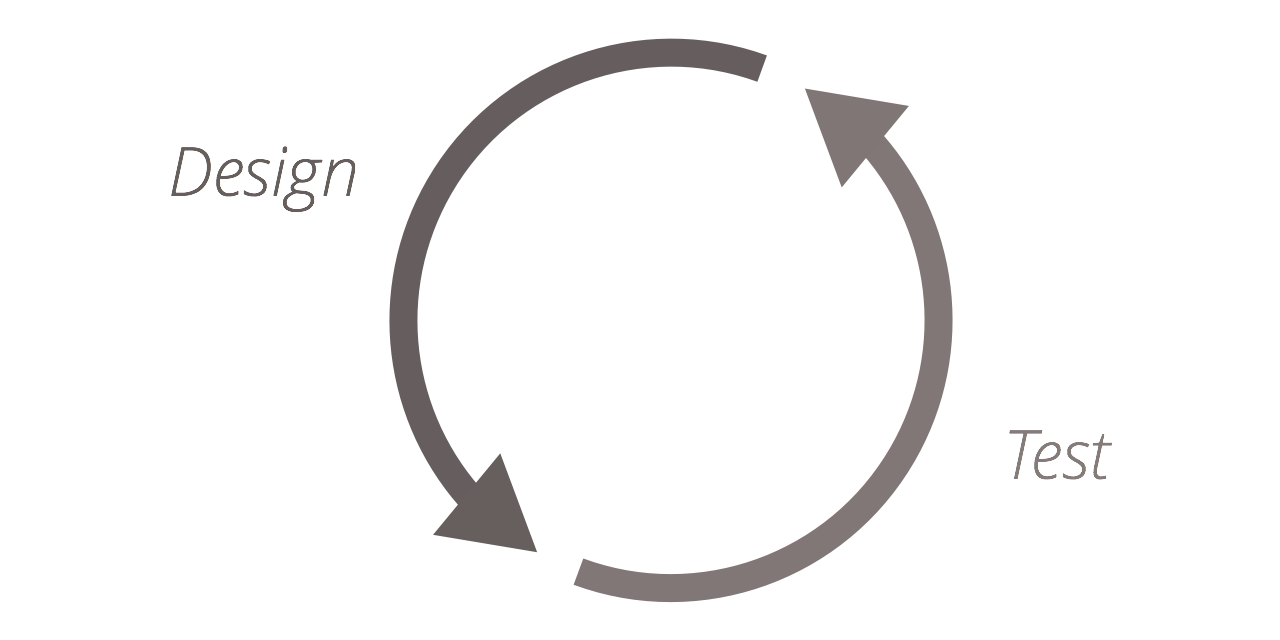
\includegraphics[width=0.8\linewidth]{Pictures/Motivation/DesignTest.png}
\end{figure}
\begin{itemize}
\item Iterative and redundant
\item Time consuming
\end{itemize}~\\
%\newline

\vfill
\columnbreak

\pause

Topology optimization
\begin{figure}
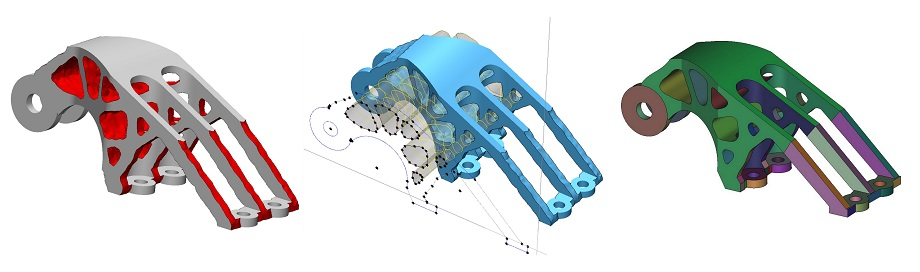
\includegraphics[width=0.9\linewidth]{Pictures/Motivation/TopOpt.jpg}
\end{figure}
\begin{itemize}
\item Promoted by additive manufacturing
\end{itemize}


\pause
\end{multicols}
\begin{tcolorbox}
\textbf{Focus}: Convert optimized geometry to \textbf{lightweight} and \textbf{scalable} CAD formats
\end{tcolorbox}

\end{frame}




%-------------------------------------------------------
\subsection{Workflow Overview}
\begin{frame}{Overview: Workflow}
	\begin{overlayarea}{\textwidth}{.1\textheight}
	\only<1>{What the user sees}
    \only<2>{CAD design including specification of loads and fixtures}
	\only<3>{Voxelized topology}
	\only<4>{Optimized topology}
	\only<5>{Surface extraction}
	\only<6>{Fit B-Spline surface}
	\end{overlayarea}
	\begin{overlayarea}{\textwidth}{.9\textheight}
    \begin{center}
		\begin{tikzpicture} 
        \uncover<1->{
        \node at (0,3)[inner sep=0pt](N1)
                {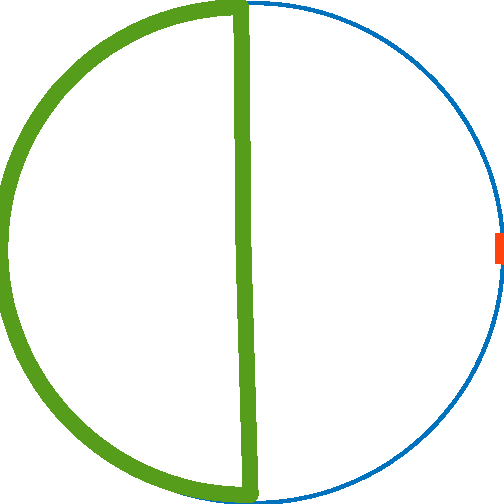
\includegraphics[width=2cm]{Pictures/1CAD_colored.pdf}};
		}
        \uncover<1->{
        \node at (0,0)[inner sep=0pt](N5)
		{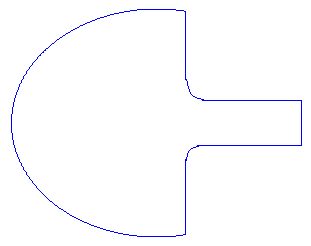
\includegraphics[width=2.2cm,height=2.2cm]{Pictures/End.png}};                        
		}        
        \uncover<1-1>{
       \draw[thick,->] (N1) -- (N5); 
		 }     
        \uncover<3->{
        \node at (4.5,3)[inner sep=0pt](N2)             
                {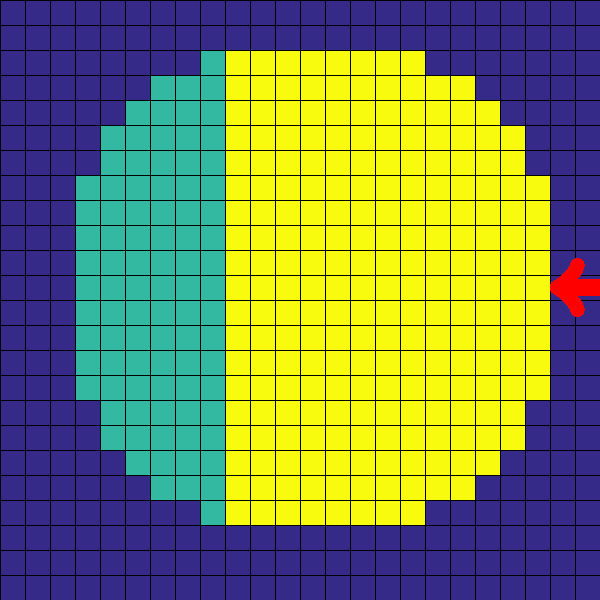
\includegraphics[width=2cm]{Pictures/4TPD.pdf}};
        \draw[thick,->] (N1) -- (N2);
        }
        \uncover<4->{
        \node at (9,1.5)[inner sep=0pt](N3) 
                {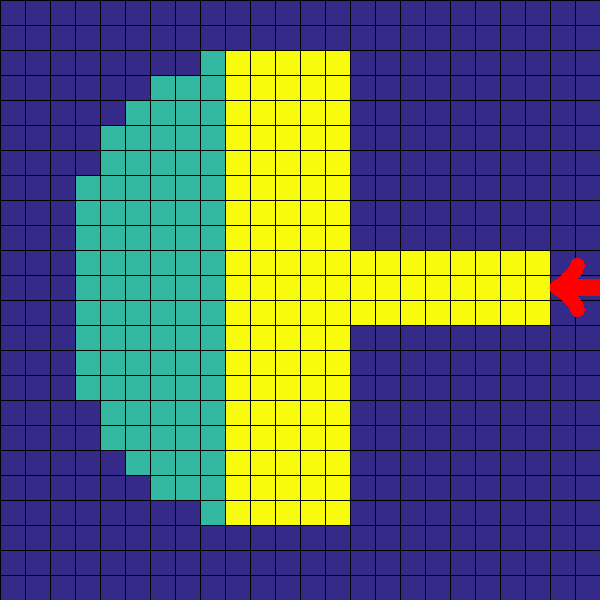
\includegraphics[width=2cm]{Pictures/5TOPOPT.pdf}};
        \draw[thick,->] (N2) -- (N3); 
        }
        \uncover<5->{
        \node at (4.5,0)[inner sep=0pt](N4)
                {
\includegraphics[width=2cm]{Pictures/7MC.pdf}};
        \draw[thick,->] (N3) -- (N4);
        }
        \uncover<6->{\draw[thick,->] (N4) -- (N5); 
        }

        \end{tikzpicture}
	\end{center}
	\end{overlayarea}

\end{frame}


%-------------------------------------------------------
\subsection{Organization}
\begin{frame}{Schedule \& Milestones}
\begin{figure}
	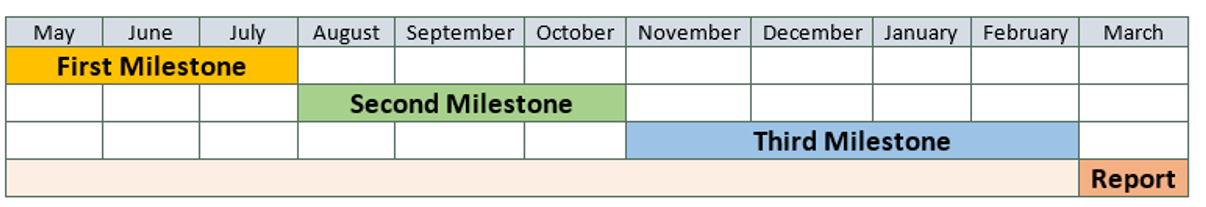
\includegraphics[scale=0.55]{Pictures/FirstHalf/timeline.png}
	\end{figure}
\end{frame}


\begin{frame}
\begin{figure}
	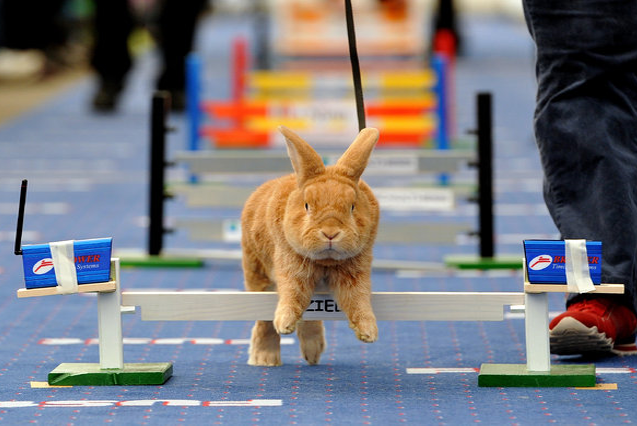
\includegraphics[scale=0.68]{Pictures/FirstHalf/bunny.png}
\end{figure}
\end{frame}

\begin{frame}{Facing the obstacles}
\begin{minipage}{1\linewidth}
\begin{multicols}{2}
Task oriented:
\begin{itemize}
\item Algorithm research 
\item Prototyping
\item Learning existing tools
\end{itemize}
\columnbreak
Organization oriented:
\begin{itemize}
\item Divide and Conquer approach
\item Flexibility to change
\item Project management
\end{itemize}
\end{multicols}
\end{minipage}

\begin{minipage}{1\linewidth}
\hspace{5 mm}
\begin{figure}
	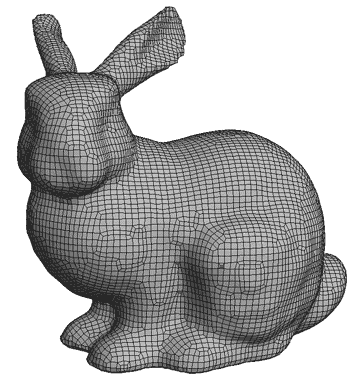
\includegraphics[scale=0.35]{Pictures/FirstHalf/sf_bunny.png}
\end{figure}
\end{minipage}

\end{frame}


\begin{frame}

	\frametitle{Project management}

	\begin{figure}
	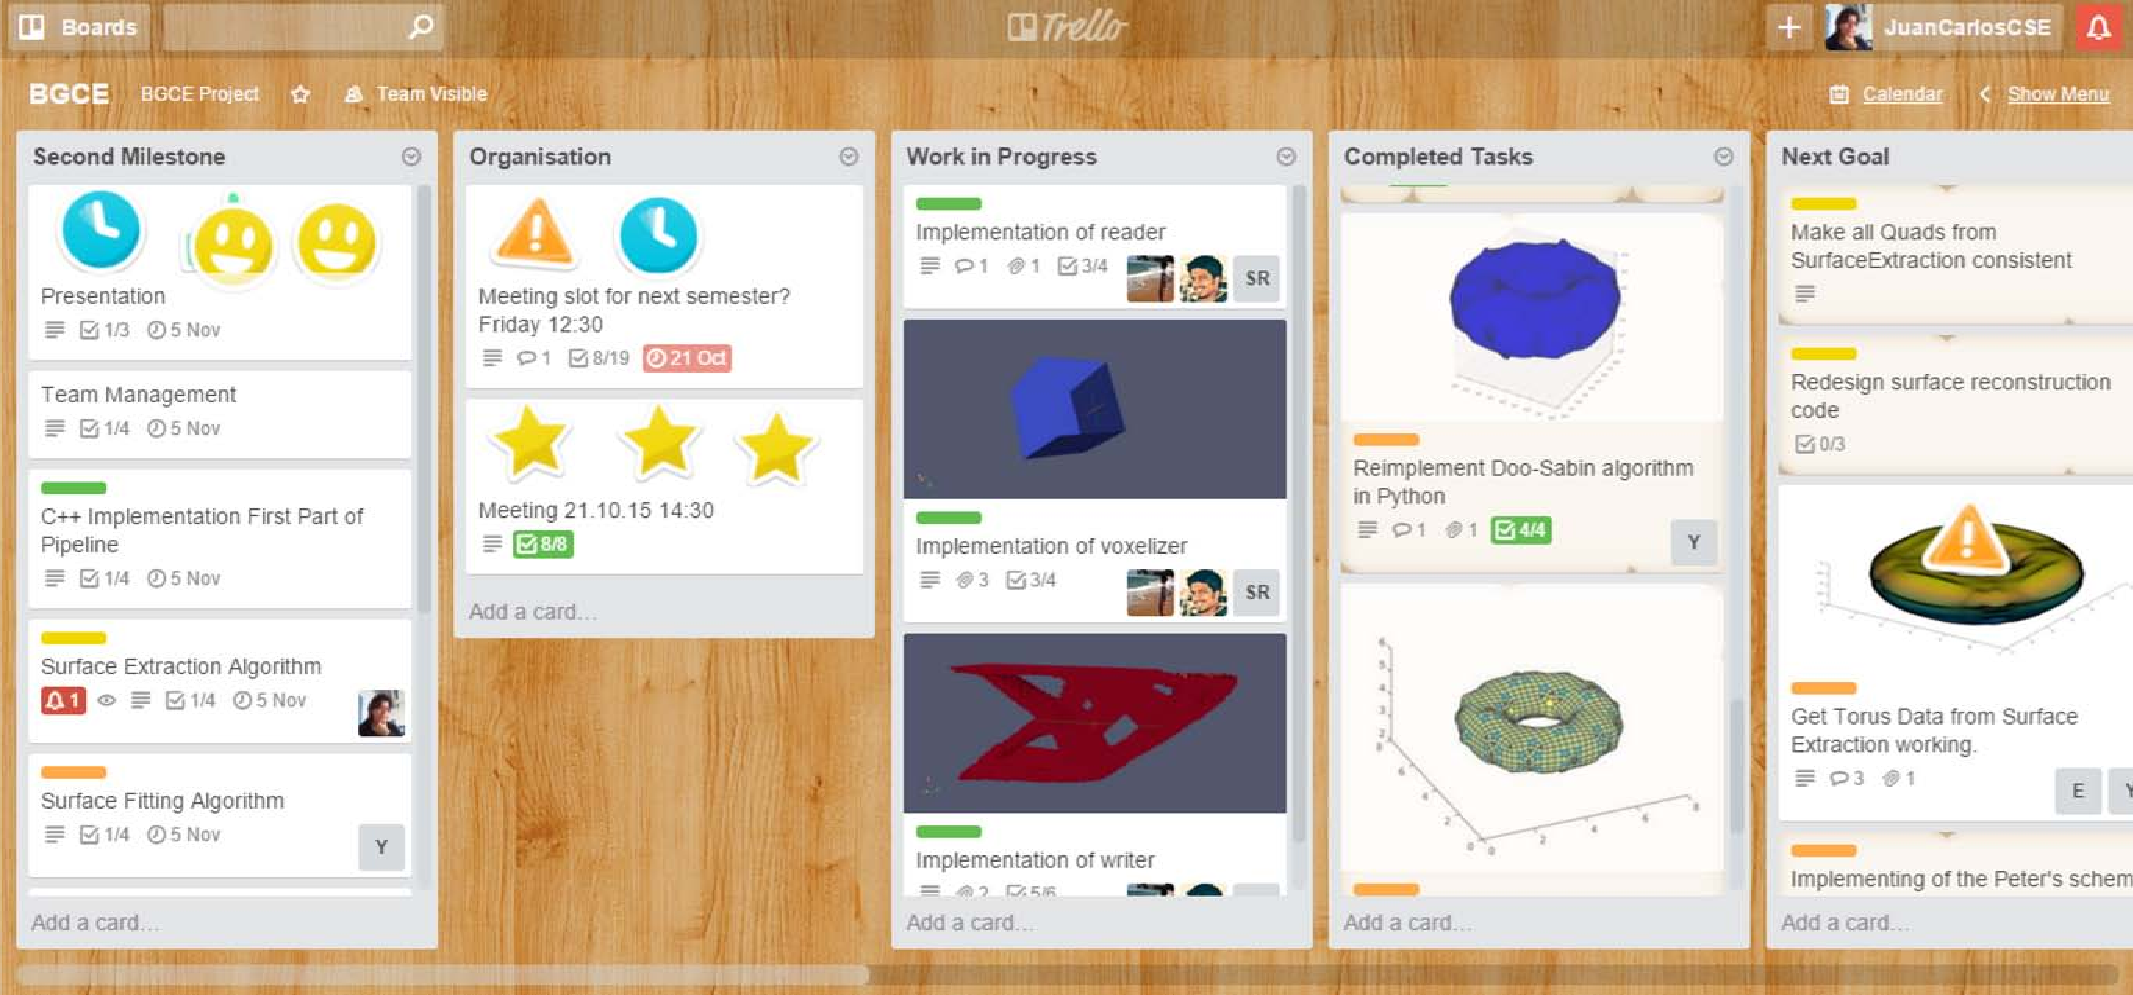
\includegraphics[scale=0.3]{Pictures/DC/Trello.pdf}
	\end{figure}
	
\end{frame}




\AtBeginSection[]
{
  \begin{frame}
  \frametitle{Contents}
  \tableofcontents[currentsection]
  \end{frame}
}

%-------------------------------------------------------
\section{Topology optimization}
\setbeamertemplate{caption}{\raggedright\insertcaption\par}

\begin{frame}{Voxelized geometry}
\begin{itemize}
\item Done using OpenCascade  
\item Each region voxelized separately 
\end{itemize}
\vspace{0.4cm}
%\begin{enumerate}
%\item Active voxels (geometry)
%\item Fixture voxels
%\item Non-changing voxels
%\item Load voxels
%\end{enumerate}
\begin{minipage}{0.49\textwidth}
\begin{figure}
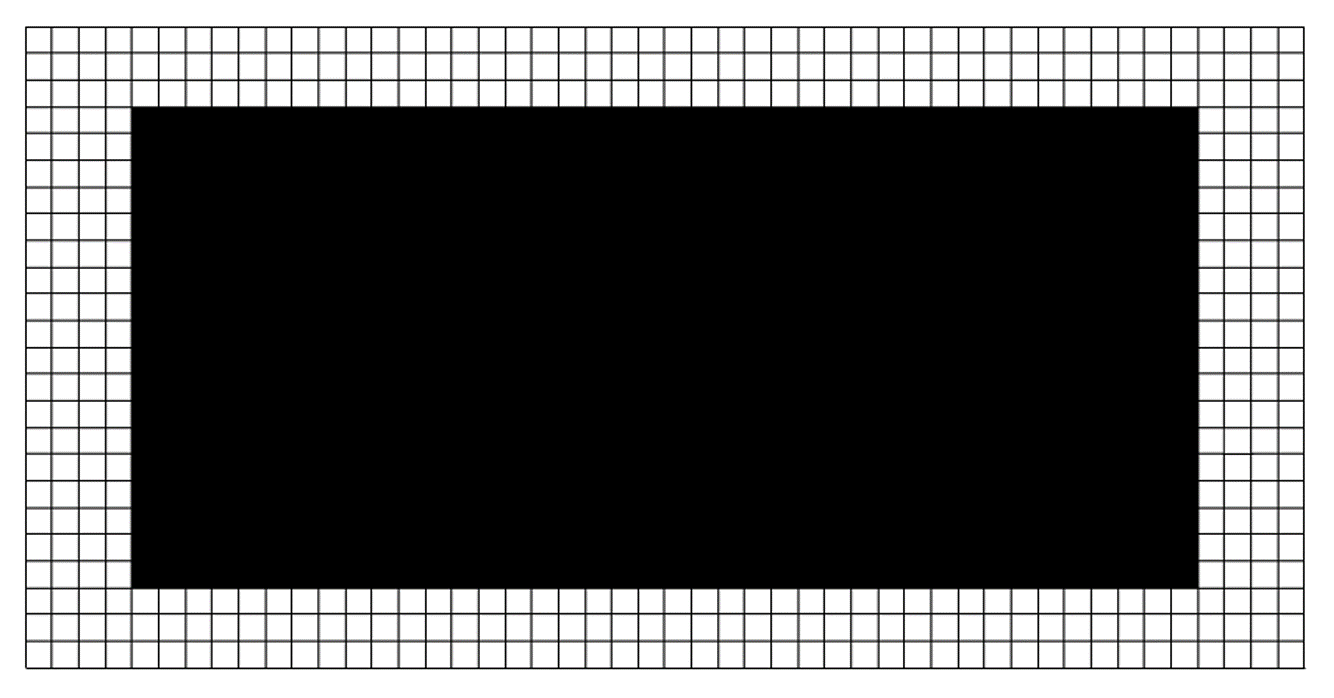
\includegraphics[width=.7\textwidth]{Pictures/Voxels/Active_2.png}
\vspace*{-2mm}
\caption{Participating voxels}
\end{figure}
\vspace{-0.6cm}
 \begin{figure}
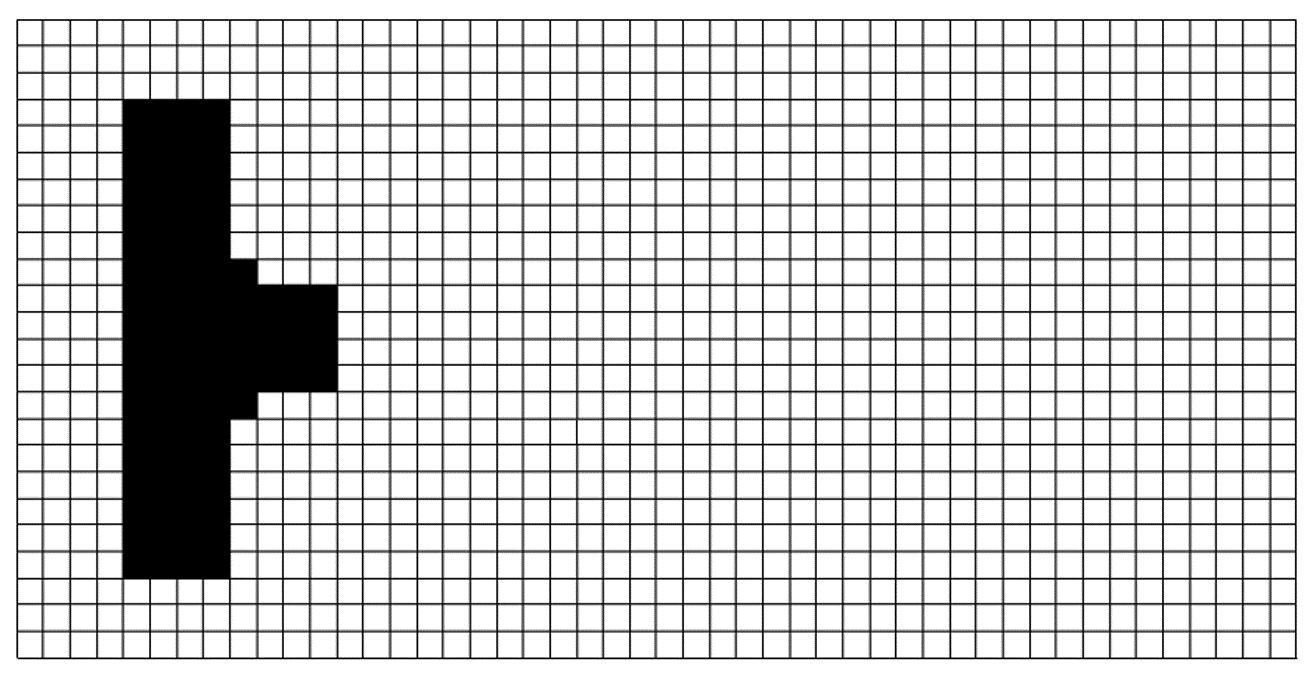
\includegraphics[width=.7\textwidth]{Pictures/Voxels/NonChanging.png}
\vspace*{-2mm}
\caption{Non-Changing Voxels}
\end{figure}
\end{minipage}
\hfill
\begin{minipage}{0.49\textwidth}
\begin{figure}

\includegraphics[width=.7\textwidth]{Pictures/Voxels/Fixture.png}
\vspace*{-2mm}
\caption{Fixture voxels}
\end{figure}
\vspace{-0.6cm}
\begin{figure}
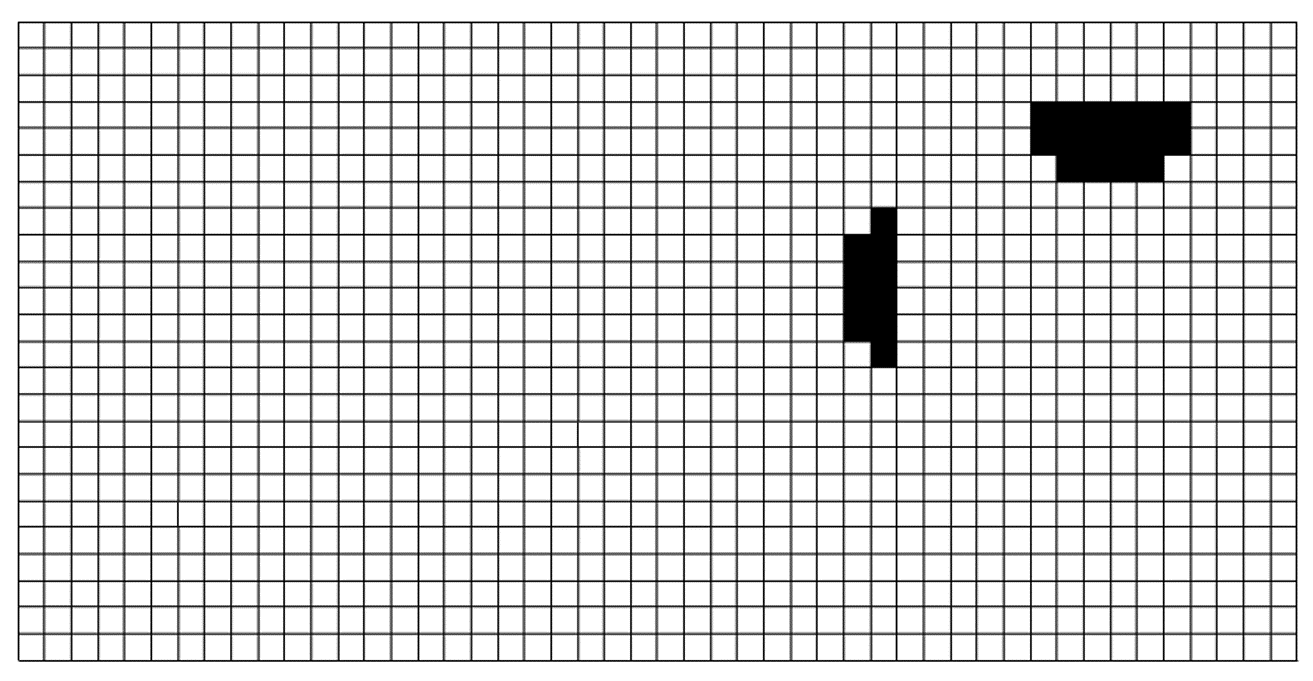
\includegraphics[width=.7\textwidth]{Pictures/Voxels/Load.png}
\vspace*{-2mm}
\caption{Load voxels}
\end{figure}
\end{minipage}
\end{frame}

\begin{frame}{Topology Optimization Process\textsuperscript{1}}
\begin{overlayarea}{\textwidth}{.8\textheight}
\begin{tikzpicture} [remember picture,overlay]
		\uncover<1->{
		\node[anchor=north,inner sep=0pt] [xshift=5cm,yshift=-0cm] (N1)
                {Provide geometry as voxel grid};
		}     
        \uncover<2->{
        \node [below =of N1, inner sep=0pt](N2){Calculate stress on each voxel};
        \draw[thick,->] (N1) -- (N2);
		}
		\uncover<3->{
		\node [right =of N2, xshift=2.5cm, inner sep=0pt](N3){};
		\node [below =of N3, yshift=-3.2cm, inner sep=0pt](N4){};
		\node [left =of N4, xshift=-2.0cm, inner sep=0pt](N5){If stress below threshold, remove voxel};
        \draw[thick,->] (N2) -- (N3) -- (N4) -- (N5);
		}
		\uncover<4->{
		\node [left =of N5, xshift=-1.3cm, inner sep=0pt](N6){};
		\node [left =of N2, xshift=-2cm, inner sep=0pt](N7){};
        \draw[thick,->] (N5) -- (N6) -- (N7) -- (N2);
		}
		\uncover<4->{
			\only<4>{
			\node [below =of N2, xshift=0.5cm, yshift=1cm](Picture){
				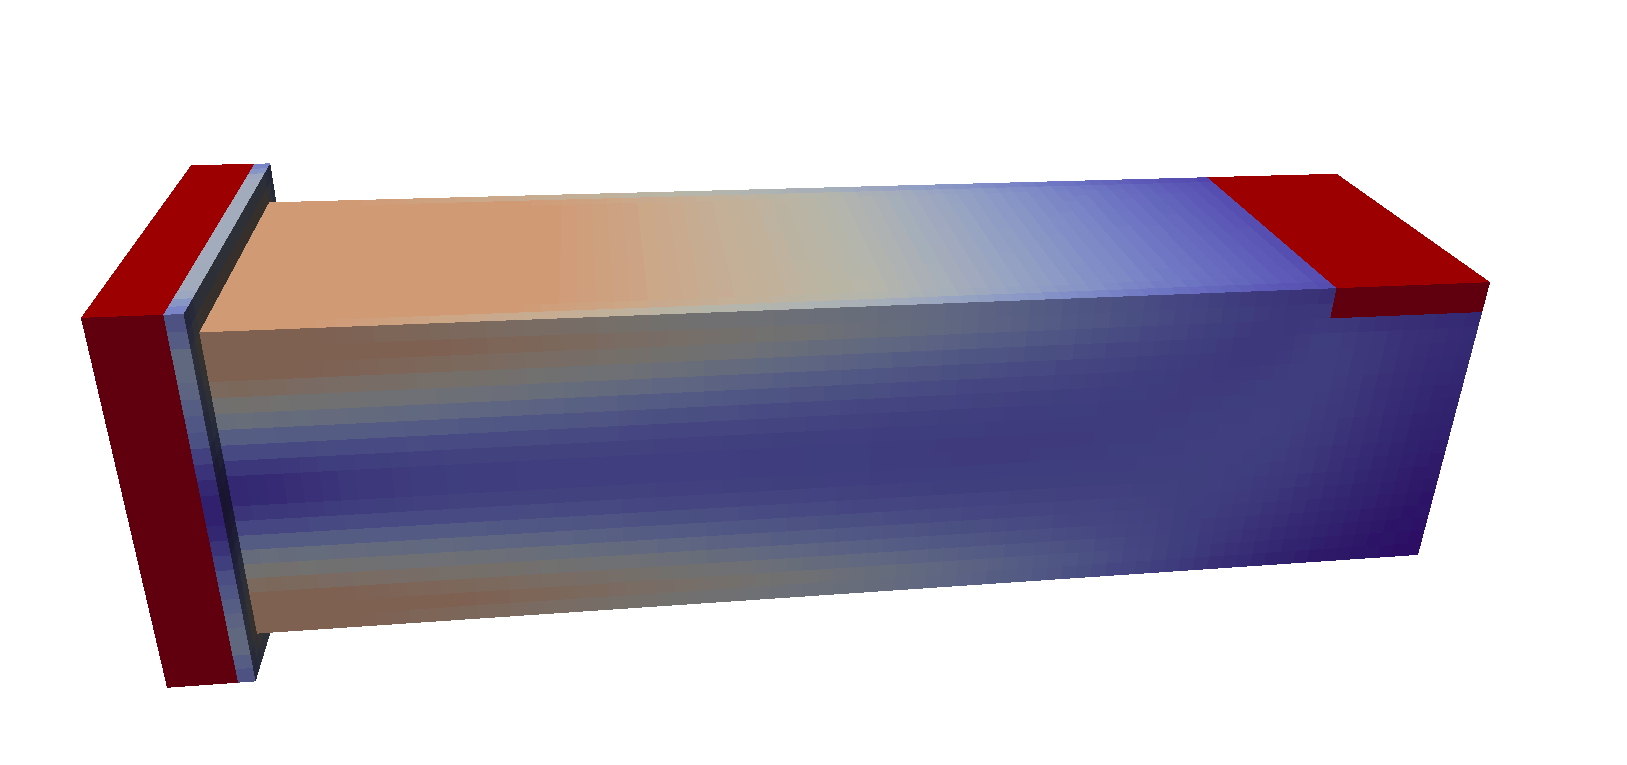
\includegraphics[scale=0.13]{Pictures/SecondHalf/Topology/Cantilever_Topy_0.png}
				};
			}	
			\only<5>{
			\node [below =of N2, xshift=0.5cm, yshift=1cm](Picture){
				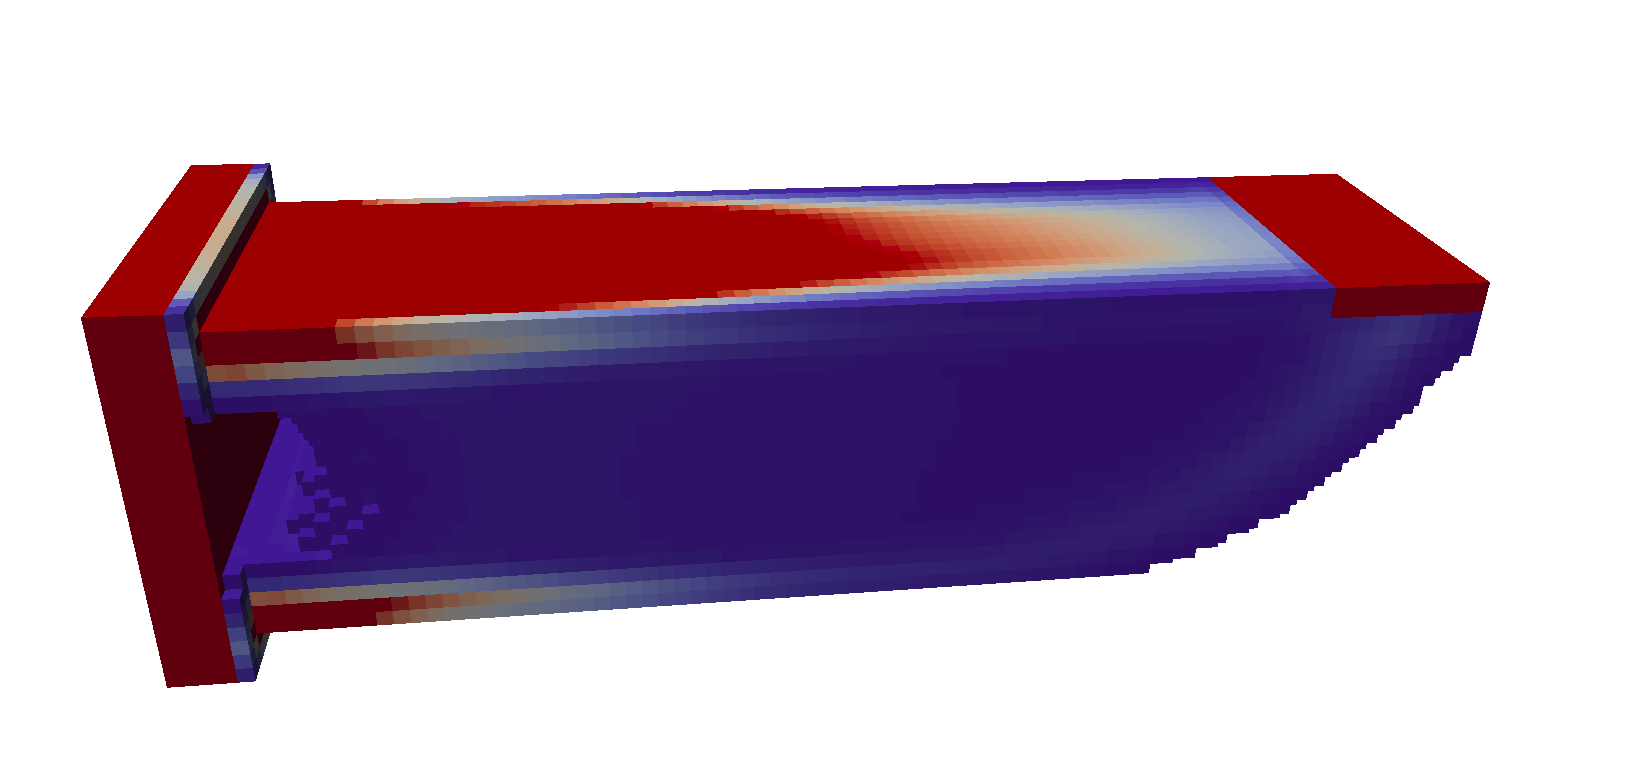
\includegraphics[scale=0.13]{Pictures/SecondHalf/Topology/Cantilever_Topy_1.png}
				};
			}	
			\only<6>{
			\node [below =of N2, xshift=0.5cm, yshift=1cm](Picture){
				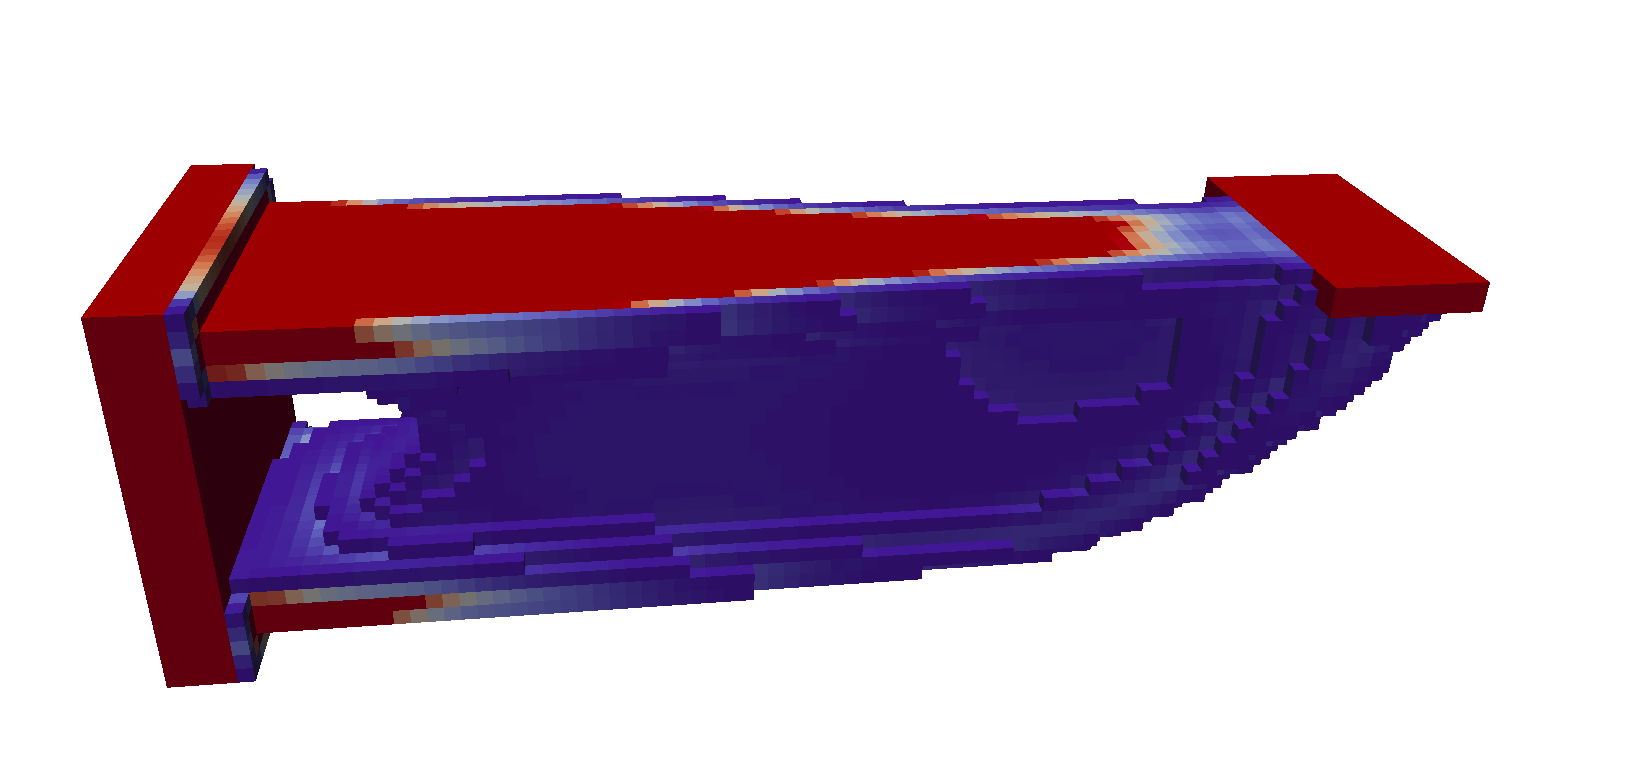
\includegraphics[scale=0.13]{Pictures/SecondHalf/Topology/Cantilever_Topy_2.png}
				};
			}	
			\only<7>{
			\node [below =of N2, xshift=0.5cm, yshift=1cm](Picture){
				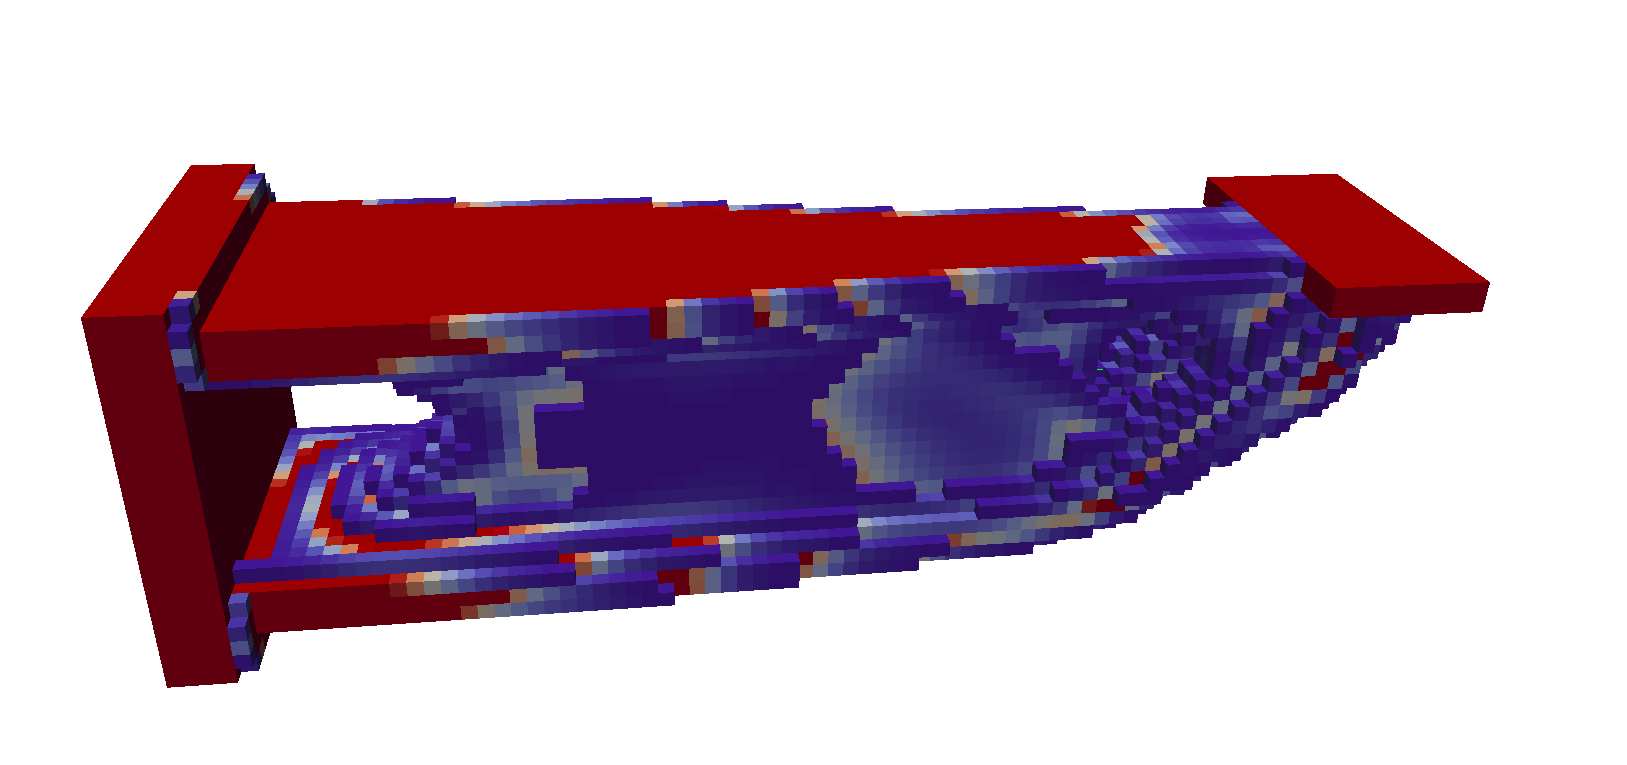
\includegraphics[scale=0.13]{Pictures/SecondHalf/Topology/Cantilever_Topy_3.png}
				};
			}	
			\only<8>{
			\node [below =of N2, xshift=0.5cm, yshift=1cm](Picture){
				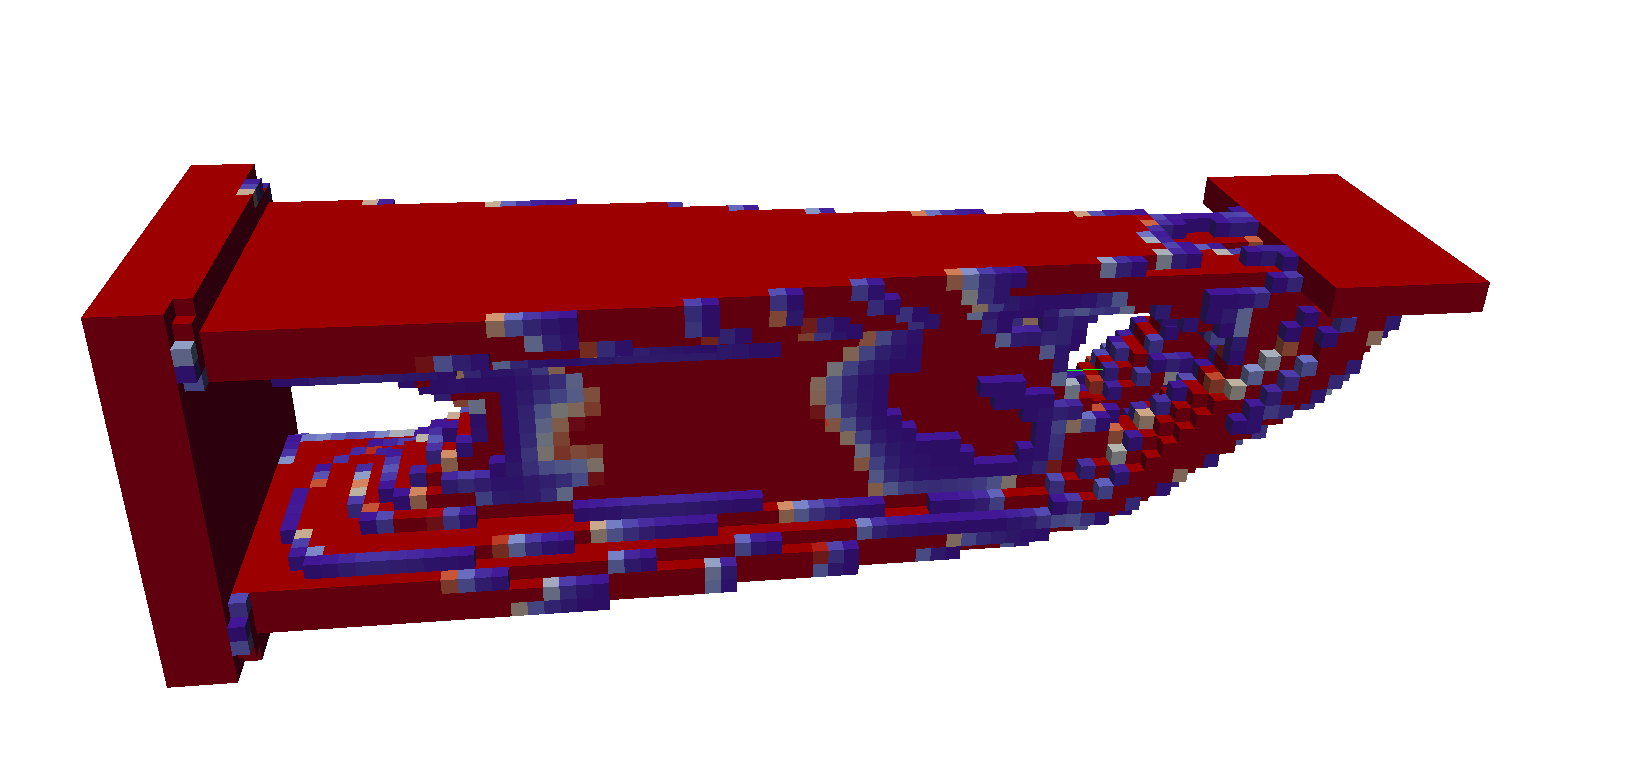
\includegraphics[scale=0.13]{Pictures/SecondHalf/Topology/Cantilever_Topy_4.png}
				};
			}	
			\only<9>{
			\node [below =of N2, xshift=0.5cm, yshift=1cm](Picture){
				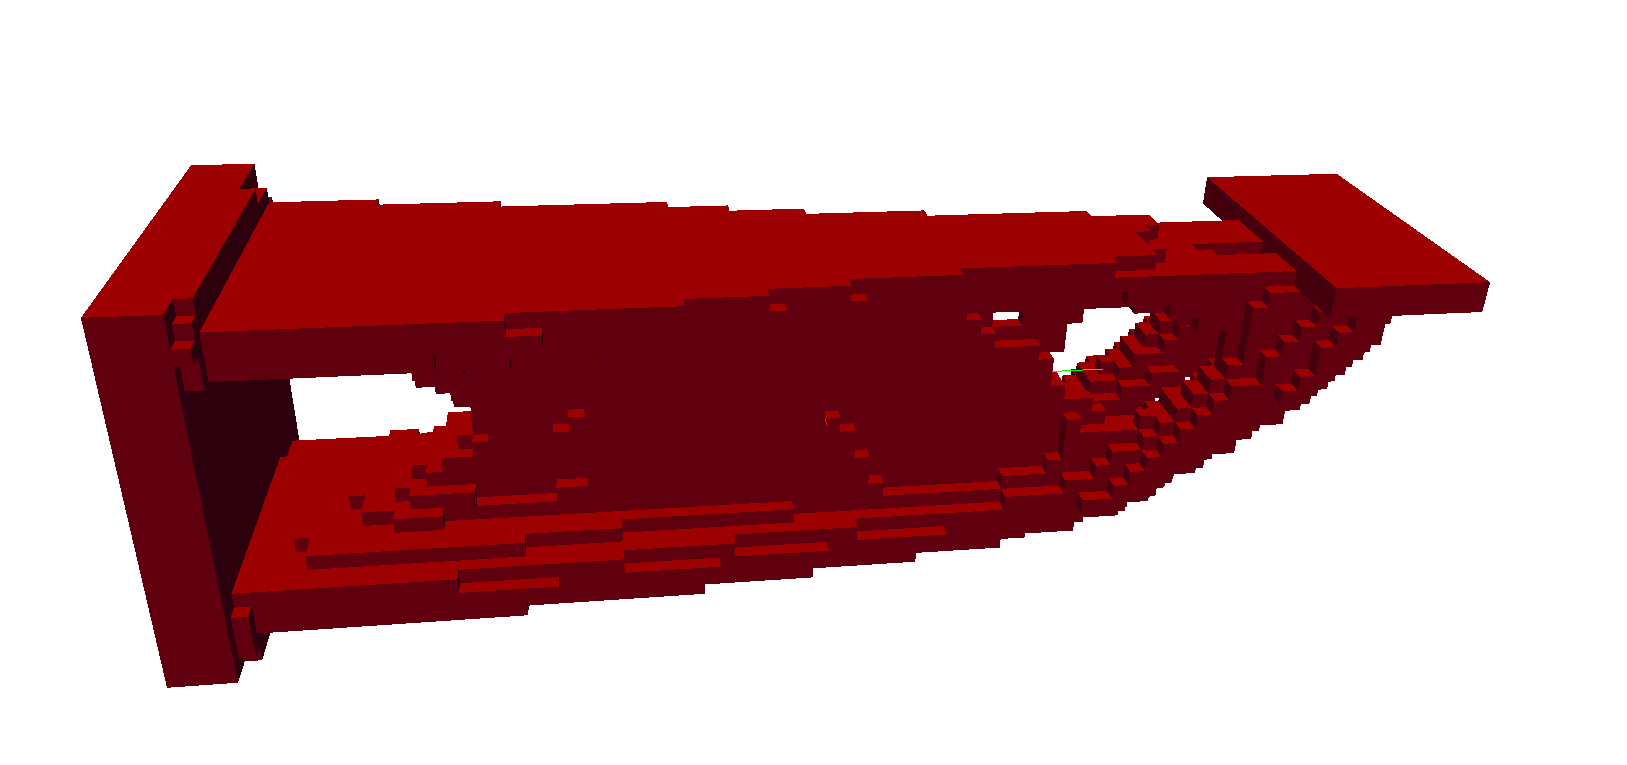
\includegraphics[scale=0.13]{Pictures/SecondHalf/Topology/Cantilever_Topy_5.png}
				};
			}	
		}
\end{tikzpicture}
\end{overlayarea}
\end{frame}

%\begin{frame}{Topology Optimization Process}
%\begin{center}
%Provide geometry as voxel grid
%$$\downarrow$$
%Calculate stress on each voxel
%$$\downarrow$$
%Remove voxel from active geometry if stress is below threshold
%\end{center}
%\end{frame}
%
%\begin{frame}{Topology Optimization Example}
%\only<1>{
%\begin{figure}
%\centering
%%\vspace{-0.5cm}
%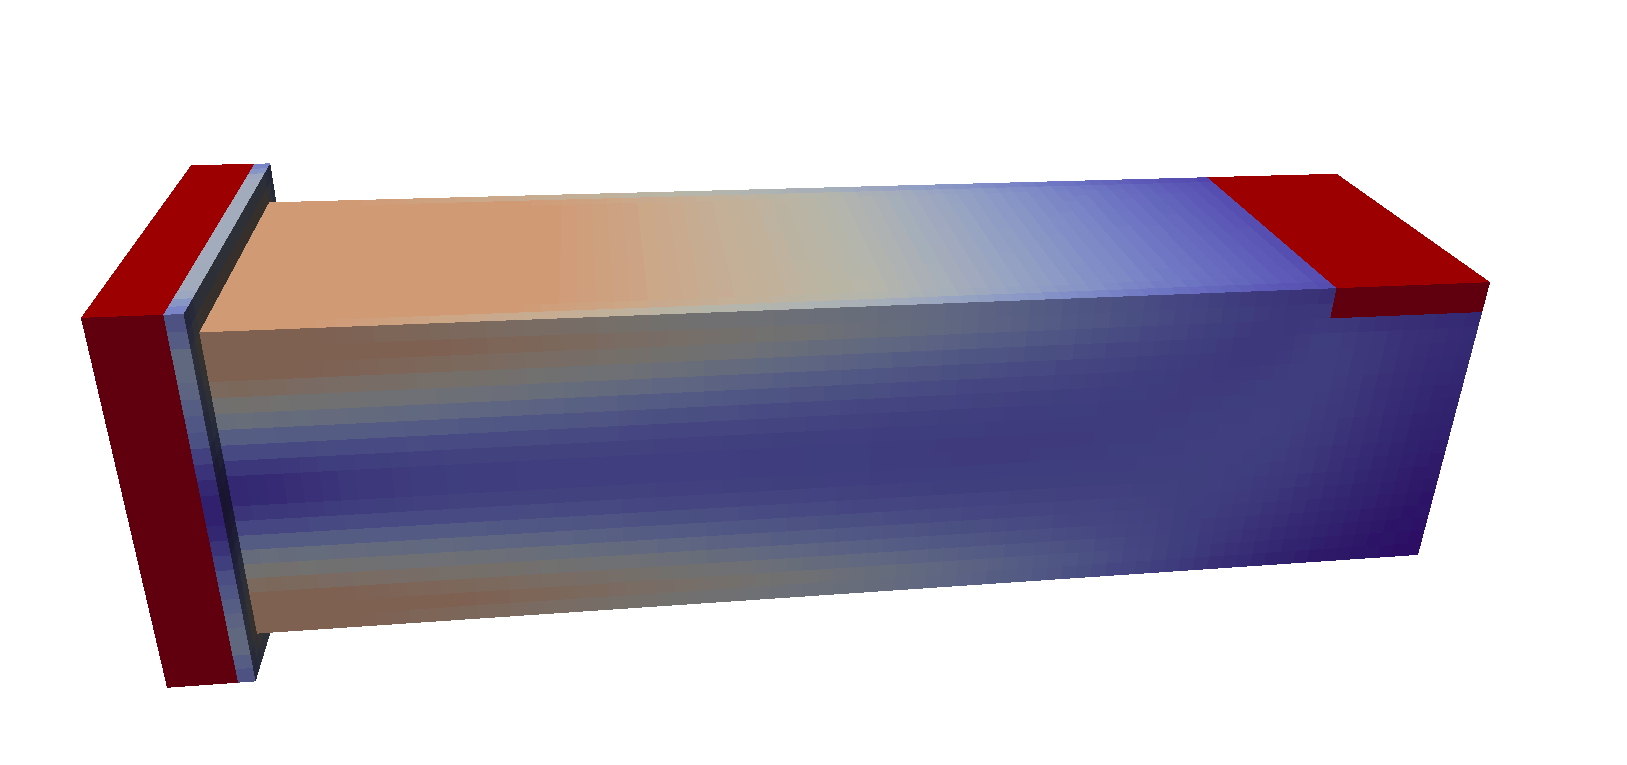
\includegraphics[width=1\textwidth]{Pictures/SecondHalf/Topology/Cantilever_Topy_0.png}
%\end{figure}}
%\only<2>{
%\begin{figure}
%\centering
%%\vspace{-0.5cm}
%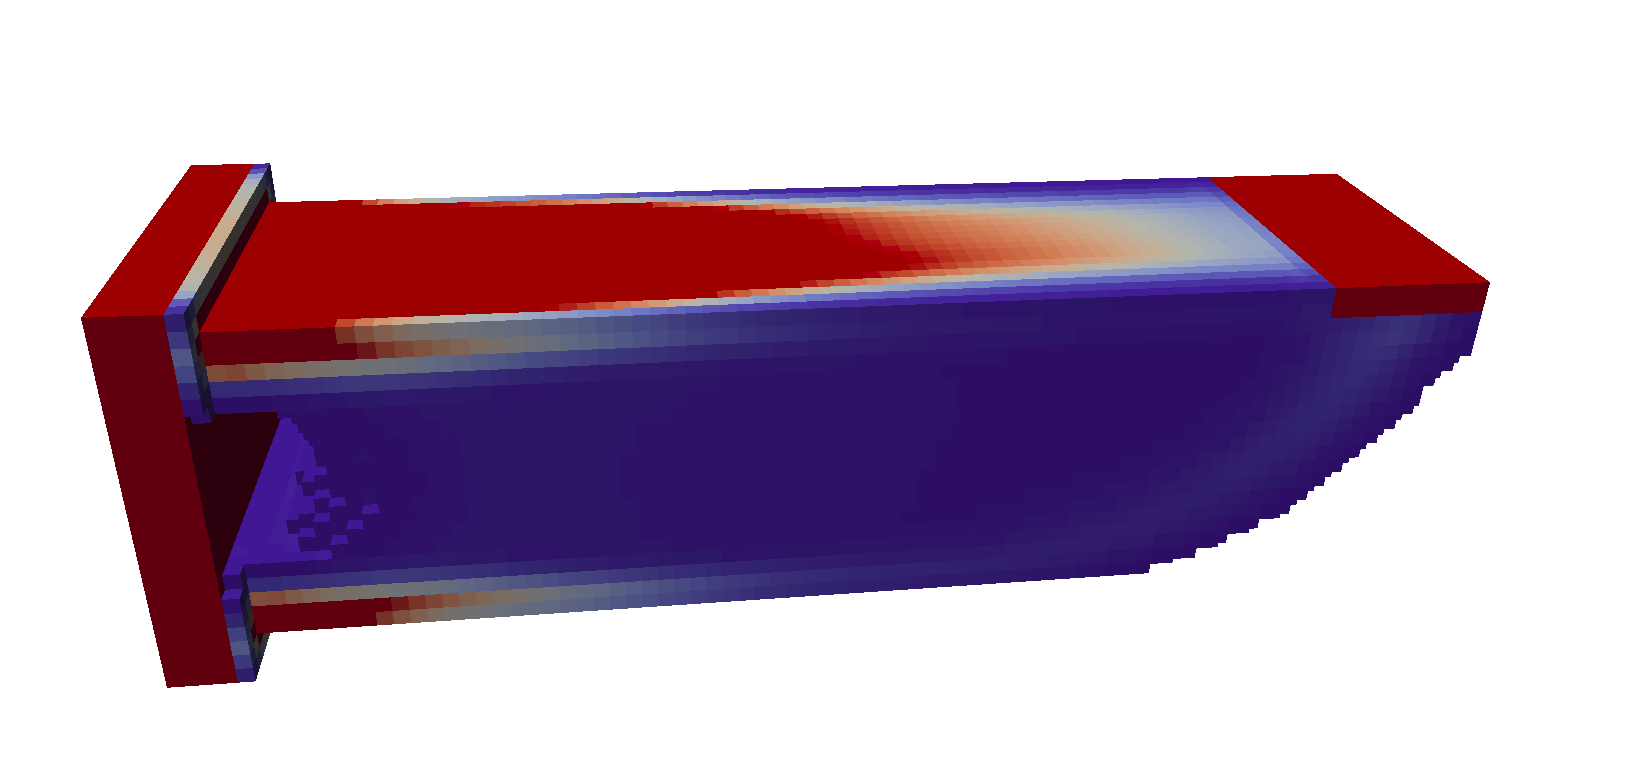
\includegraphics[width=1\textwidth]{Pictures/SecondHalf/Topology/Cantilever_Topy_1.png}
%\end{figure}}
%\only<3>{
%\begin{figure}
%\centering
%%\vspace{-0.5cm}
%\includegraphics[width=1\textwidth]
%{Pictures/SecondHalf/Topology/Cantilever_Topy_2.png}
%\end{figure}}
%\only<4>{
%\begin{figure}
%\centering
%%\vspace{-0.5cm}
%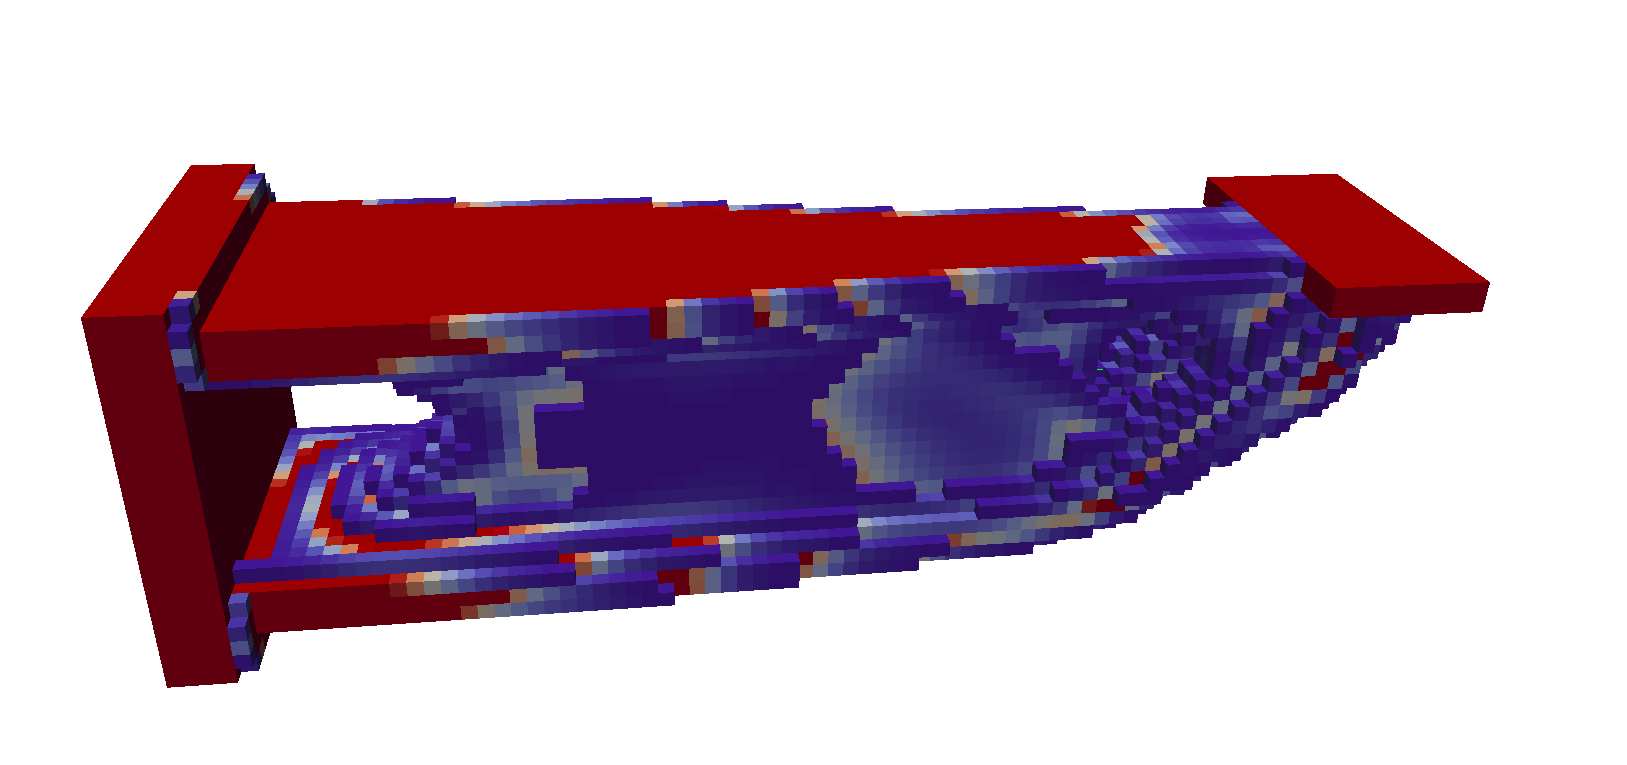
\includegraphics[width=1\textwidth]{Pictures/SecondHalf/Topology/Cantilever_Topy_3.png}
%\end{figure}}
%\only<5>{
%\begin{figure}
%\centering
%%\vspace{-0.5cm}
%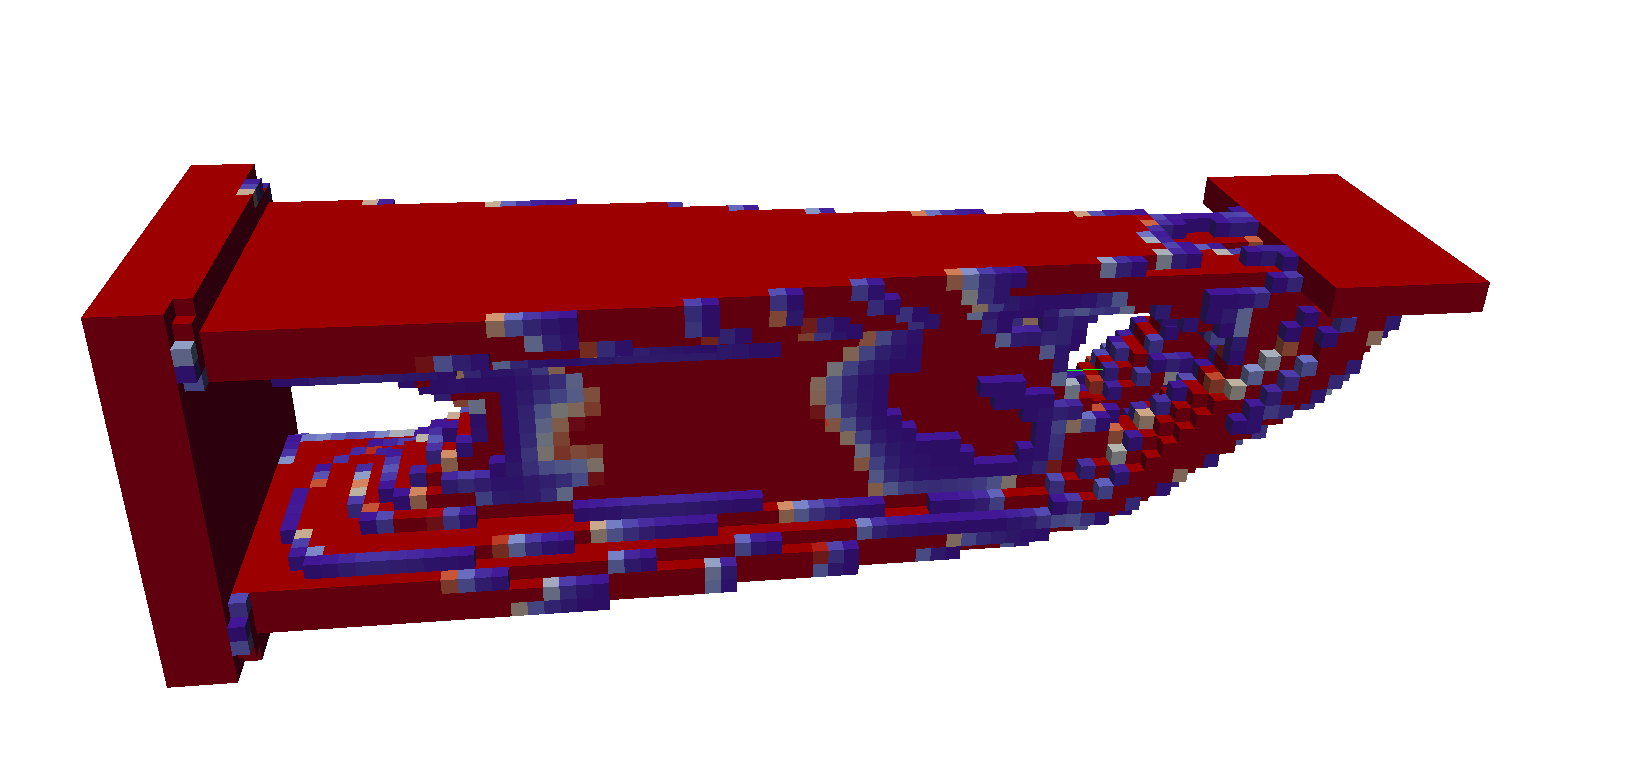
\includegraphics[width=1\textwidth]{Pictures/SecondHalf/Topology/Cantilever_Topy_4.png}
%\end{figure}}
%\only<6>{
%\begin{figure}
%\centering
%%\vspace{-0.5cm}
%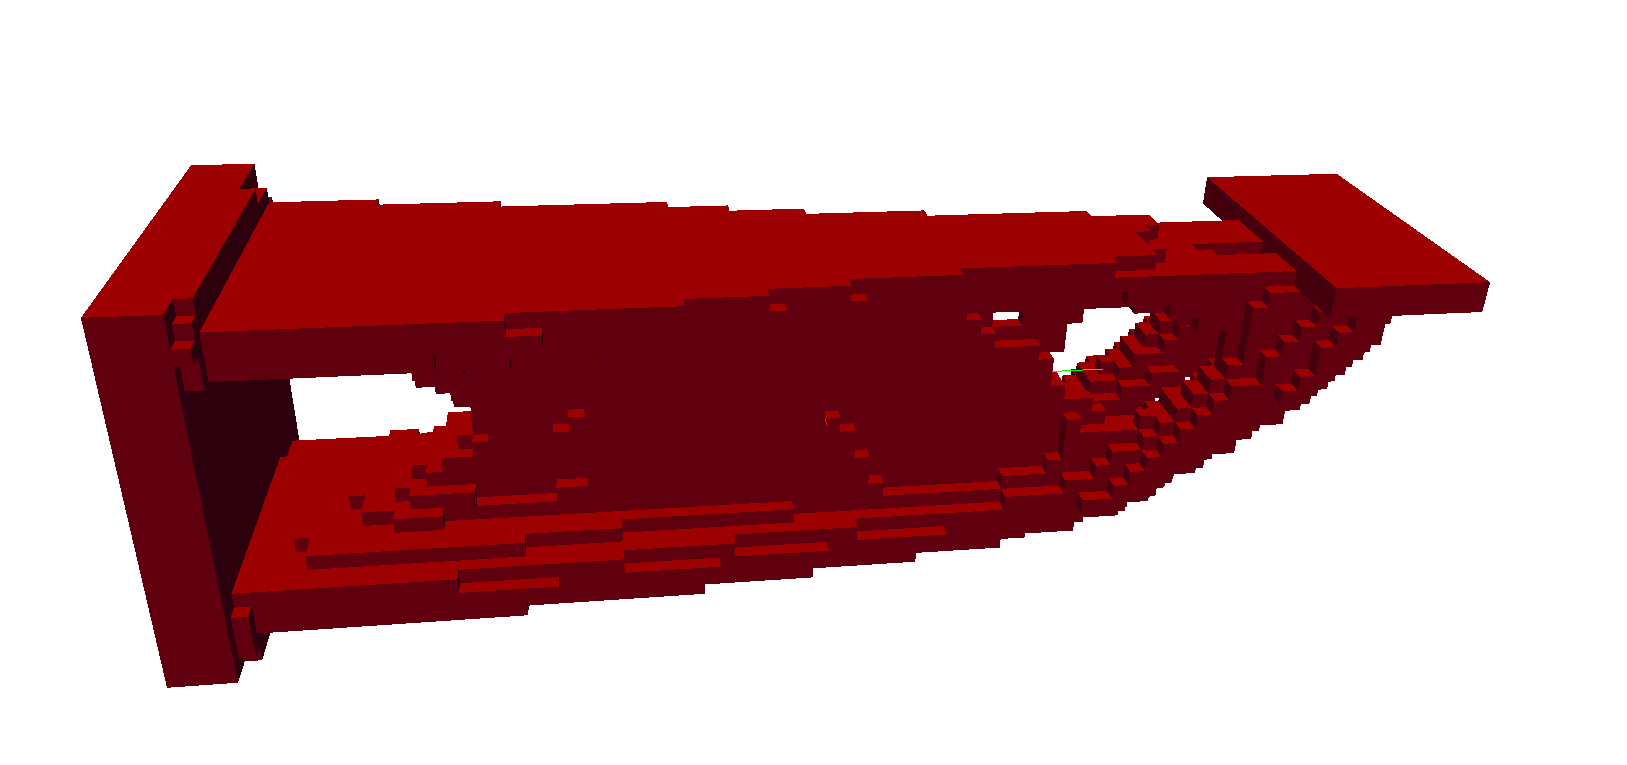
\includegraphics[width=1\textwidth]{Pictures/SecondHalf/Topology/Cantilever_Topy_5.png}
%\end{figure}}
%\end{frame}

%-------------------------------------------------------

%-------------------------------------------------------
%
\section{Surface Extraction}
%BEGIN JC
\subsection{Isosurface Contouring}
Now when the optimized voxel data was obtained, the next step is to generate a \emph{mesh based
geometry}. It will be useful in the further NURBS implementation. In order to achieve it, the
data will be represented by a contour of a smooth function, rendering an isosurface. The
isosurface allows to visualize Scalar Volumetric Data in 3D. It furthermore permits a mesh
representation of the volume data. The mesh can be composed of triangles or quads, according
to the algorithm used. There are two main approaches to solve this problem, the most
famous one is Marching Cubes.

\begin{figure}
\centering
   \scalebox{0.8}{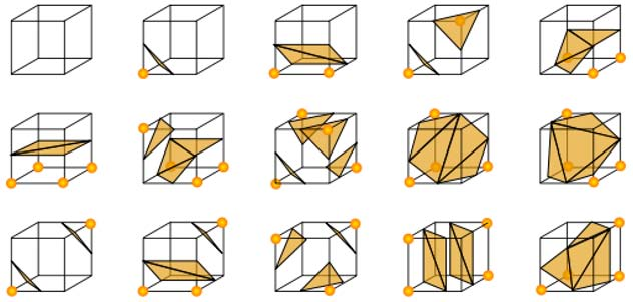
\includegraphics{Pictures/cubes.pdf}}\\
   \caption{Basis cases of Marching Cubes}
\end{figure}

\subsubsection{Marching Cubes} 

This algorithm takes as an input a regular volumetric data set and extracts a polygonal mesh. It
divides the space into cubes, which are defined by the volume information. Each cube has scalar
information on its vertices, the value is equal or above a marked isovalue. Therefore each of the
eight vertices of a cube can be marked or unmarked. According to these values vertices are drawn
on the edges of the cube at calculated points with the use of interpolation. A cube that contains
an edge is called active. Non active cubes are not further considered in the algorithm.

By connecting the vertices we obtain a polygon on each cube. There are 256 possible scenarios,
but most of them are just reflections or rotationally symmetric cases of each other. Therefore
there are 15 base cases which represent all the possibilities of the marching cubes (Figure 2.1). 
The original algorithm presents two main problems. Firstly it does not guarantee neither
correctness nor topological consistency, which means that holes may appear on the surface due
to inaccurate base case selection. The second problem is ambiguity, which appears when two
base cases are possible and the algorithm chooses the incorrect one. These cases can be grouped
into face ambiguities and internal ambiguities. There are many extended Marching Cubes
algorithms that tackle the problems of the original one, getting rid of the ambiguities and
providing correctness.

\subsubsection{Dual Contouring}
The idea of this algorithm is similar to Marching Cubes, but instead of generating vertices on the
edges of the cubes, it locates them inside the cube. Figure 2.5 shows the basic differences in both approaches.
The vertices associated with the four contigous cubes are joined and form a quad. The question now is
which place inside the cube is the ideal one to insert each vertex. Different dual algorithms are classified 
according to the answer for this question. Dual contouring generates a vertex positioned at the minimizer of a
quadratic function which depends on the intersection points and normals. Therefore the method needs Hermite 
data to work with.
\begin{equation*}
E(x)= x^TA^TAx-2x^TA^Tb+b^Tb
\end{equation*}
Where \textit{A} is a matrix whose rows are the normals and \textit{b} is a vector whose entries are the product of normals and intersection points. To solve this system, a nummerical treatement is needed. As proposed in [1] the best approach is to compute the
SVD decomposition of \textit{A} and form the pseudo-inverse by truncating its small singular values. 
%1=Dual Contouring of HErmite DAta


The main advantage of this method over MC is the adquisition of better aspect ratios. On the other hand the need of Hermite Data
represents a disadvantage. Furthermore there is no open source algorithm that implements the Dual Contouring scheme.


\subsection{The VTK Toolbox}
\subsubsection{Installing VTK}
VTK was installed using the Linux platform, for it to be successfully implemented a gcc compiler
must be already on the machine. VTK offers the possibility to use Python, TLC or C++ for
development. VTK toolbox is actually a C++ library, which is implemented in other languages. We
decided to continue the project with C++ since it gives the possibility to explore the original code.
A few dependency problems were encountered, nevertheless they were easy to track back. If any
problems were to be found at installation time, please refer to the VTK Wiki where the procedure
is explained step by step.

\begin{figure}
\centering
   \scalebox{0.35}{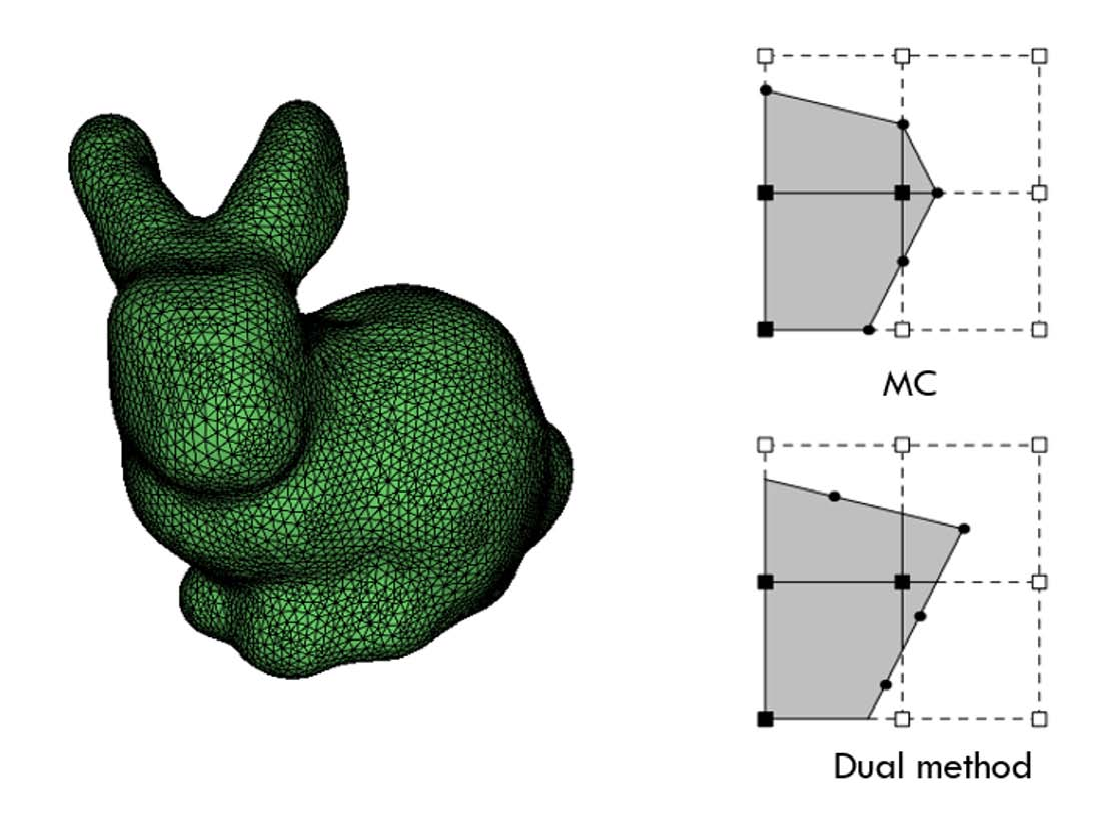
\includegraphics{Pictures/bunny_MC.pdf}}\\
   \caption{\textit{Right:} The famous Standford Bunny. \textit{Left:} Main difference between MC and Dual methods }
\end{figure}

\subsubsection{Implementing the VTK Classes}
The VTK toolbox was used in order to implement the algorithms on our optimized data. It is a heavily object
oriented toolbox. Our first approach was to use the built in Marching Cubes algorithm,
nevertheless it did not work with our unstructured grid data. It just works for ImageData and
PolyData . For structured and unstructured grids the tool to render the isosurface is the contour
Filter tool. Unfortunately the documentation does not present which algorithm the tool uses. It
can be inferred that it is an extended Marching cube algorithm.

The Contour Filtering seemed to work fine but the visualization of our data was still not possible
and an intermediate step was needed. We used the Implicit Modelling tool which is a filter that
computes the distance from the input geometry to the points of an output structured point set.
This distance function can then be "contoured" to generate new, offset surfaces from the original
geometry. It finally allowed visualization but it created one problem. Holes are lost in
the process.

\begin{figure}
\centering
   \scalebox{0.4}{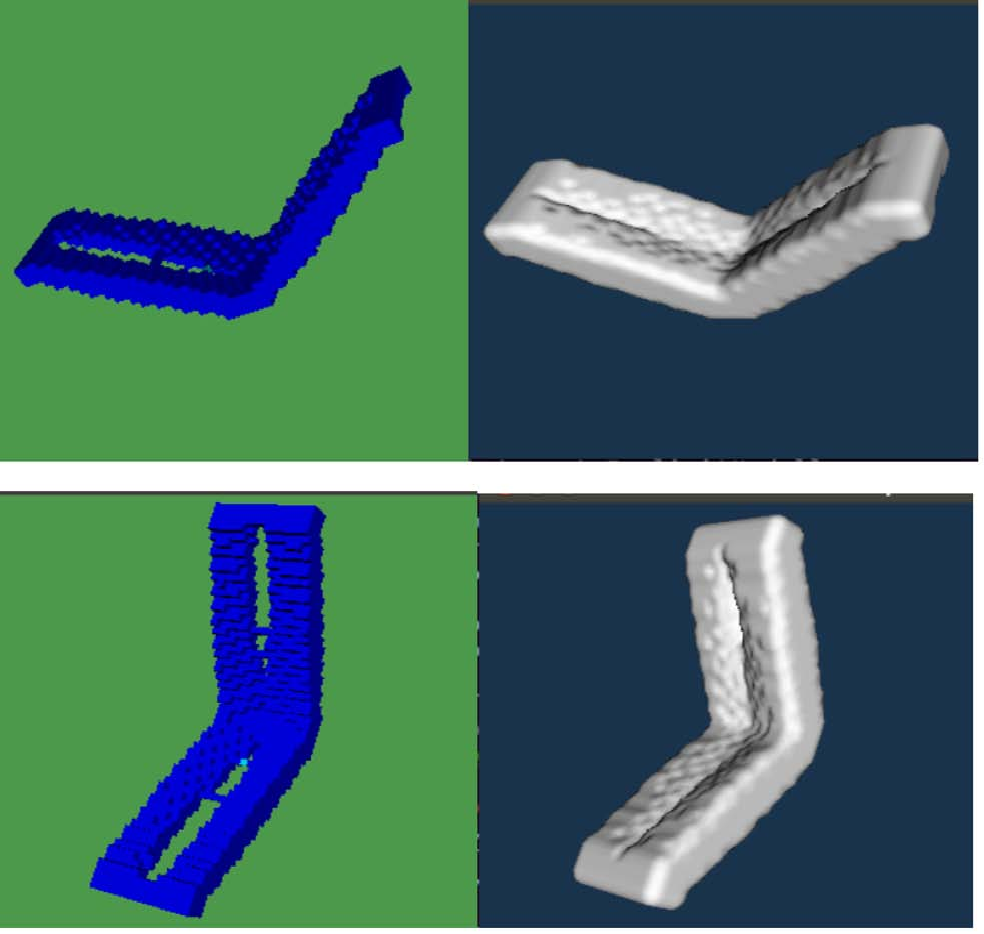
\includegraphics{Pictures/contouring.pdf}}\\
   \caption{Contour Filtering tool after Implicit Modelling}
\end{figure}

A further idea to solve this problem is to convert at the first step the volume data into point data
and only then present it to the Contour Filtering Tool. This will be implemented in the next
milestone.

The next step was to create a coarser mesh from the fine one. The triangles that represent the
isosurface can be reduced with the Decimation tool. A smoothing step is necessary in between
to get the new connections right. The top part of figure [2] shows a 50 \% reduction of the
triangles, a noticeable difference can not be perceived. On the lower part a 90 \% reduction is
obtained, it is nevertheless still difficult to see a difference. Triangle meshes can be easily
coarsened since there are many open source algorithms that simplify the triangles. VTK has the
decimation tool which works for 3D triangle data.

\begin{figure}
\centering
   \scalebox{0.4}{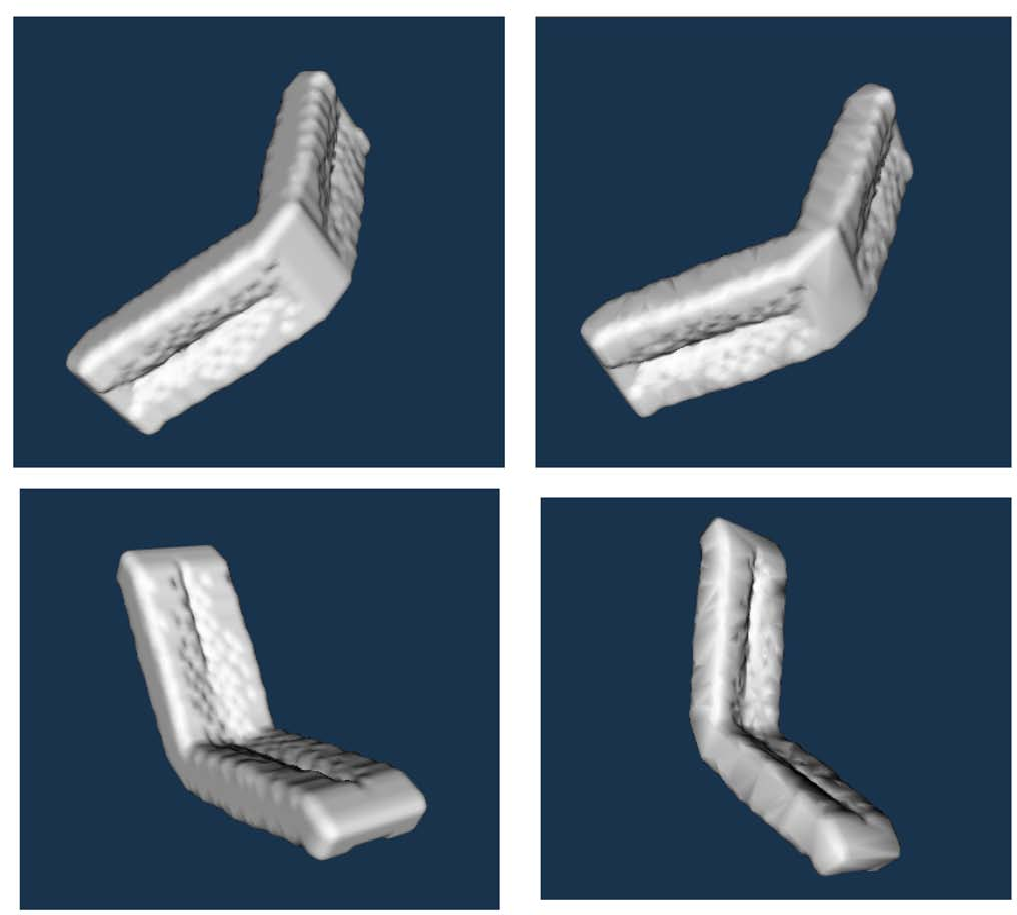
\includegraphics{Pictures/Decimation.pdf}}\\
   \caption{Decimation of triangles. \textit{Top:} 50\% \textit{Lower:}90\%}
\end{figure}

\subsection{The Long Road to NURBS}
There are two possible roads to go from the voxel data to the NURBS representation.
\subsubsection{Quad Contouring}
This approach uses the dual contouring algorithm as first step in order to obtain a quad mesh
representation from the voxel data. The first challenge is to implement correctly the algorithm
with the ideas presented in [1]. The original marching cubes algorithm is
implemented in VTK but the source code is not public, therefore not only an extension
of it is needed, but a full implementation. Once this first step is done, the quads will be chosen for the
NURBS parametrization. A second step considers multiple smaller quads which have to be
combined into one larger patch. This is another challenge, since the remeshing of quad meshes
is not as straight forward as with the triangles. Different approaches have been taken in order to
achieve this coarsening. In [2] an incremental and greedy approach, which is based on local operations only, is presented. It depicts an iterative process which performs local optimizing, coarsening and smoothing operations. Another approaches, like
the one presented in [3] uses smooth harmonic scalar fields to simplify the mesh.
%2= “Practical quad mesh simplification”
%3= “Harmonic Functions for Quadrilateral Remeshing of Arbitrary Manifolds”


\subsubsection{Multiresolution Analysis of Arbitrary Meshes}
With this approach there is no need to apply a Dual Contouring algorithm, since it takes as
beginning data the triangles from the Marching Cubes. The main concepts are shown in the paper
of the same name [4]. It mainly takes a series of intermediate steps which permits a parametrization of data. It includes a partitioning scheme based on the ideas of the Voronoi Diagrams and Delaunay triangulations. Large patches or quads are obtained with this method. Further discussion on this approach is explained in the following section.

%4=reference to MAAM, a.k.a Benni's favorite paper!

Both approaches have not been implemented in open source documentation, therefore it will be
a long road to achieve what is required. For the first part the second
road was chosen and in case it leads to a dead end, the first way will be taken into consideration.

%END JC


\section{B--Spline Fitting}
\newcommand{\norm}[1]{\parallel #1 \parallel_2}
%\subsection{B--Spline}
\begin{frame}{Least sqare fitting problem}
\begin{overlayarea}{\textwidth}{.15 \textheight}
\begin{enumerate}
\item Coarse approximating quad from Dual Contouring
\item<2-> Projection of datapoint onto plane
\item<3-> Task: Find corresponding parameters for B-Spline surface $\left[u,v\right] \in \left[0,1\right]^2$
\end{enumerate}
\end{overlayarea}
\begin{overlayarea}{\textwidth}{.85 \textheight}
\begin{columns}
\column{.35\textwidth}

\begin{overlayarea}{\textwidth}{\textheight}
\begin{figure}
\only<1-4>{
\tdplotsetmaincoords{60}{110}
\begin{tikzpicture}[scale = 1.5,tdplot_main_coords]
\coordinate (O) at (-1,-1,0);
\coordinate[dot] (A) at (0,0,0);
\coordinate[dot] (B) at (1,0,0);
\coordinate[dot] (C) at (1.2,1.5,0);
\coordinate[dot] (D) at (0,1,0);
\only<3->{
\coordinate[dot] (E) at (1.4,2.0,-0.5);
\coordinate[dot] (F) at (0,1.7,-0.8);
\draw[thick] (D) -- (F) -- (E) -- (C);}

\coordinate (P1) at (.5,.4,1);
\coordinate (P2) at (1,1,1);
\coordinate (P3) at (0.2,0.2,2);
\coordinate (P4) at (0.1,1.3,1);


\coordinate (Q1) at (.5,.4,0);
\coordinate (Q2) at (1,1,0);
\coordinate (Q3) at (0.2,0.2,0);
\coordinate (Q4) at (0.1,0.9,0);



\draw[thick,->] (O) -- ($(O)+(.5,0,0)$) node[anchor=north east]{$x$};
\draw[thick,->] (O) -- ($(O)+(0,.5,0)$) node[anchor=north west]{$y$};
\draw[thick,->] (O) -- ($(O)+(0,0,.5)$) node[anchor=south]{$z$};

\draw[thick] (A) -- (B) -- (C) -- (D) -- (A);

\only<2-4>{
\draw (P1) node[thick,cross,red,label = {$P_1$}] {};
\draw[red,dashed] (P1) -- (Q1);
\draw (Q1) node[thick,cross,red] {};
\draw (P2) node[thick,cross,red,label = {$P_2$}] {};
\draw[red,dashed] (P2) -- (Q2);
\draw (Q2) node[thick,cross,red] {};
\draw (P3) node[thick,cross,red,label = {$P_3$}] {};
\draw[red,dashed] (P3) -- (Q3);
\draw (Q3) node[thick,cross,red] {};
}
\only<3->{
\draw (P4) node[thick,cross,red,label = {$P_4$}] {};
\draw[red,dashed] (P4) -- (Q4);
\draw (Q4) node[thick,cross,red] {};

}
\draw (A) node[label = left:{$A$}]{};
\draw (B) node[label = left:{$B$}]{};
\draw (C) node[label = right:{$C$}]{};
\draw (D) node[label = right:{$D$}]{};
\only<3->{
\draw (E) node[label = right:{$E$}]{};
\draw (F) node[label = right:{$F$}]{};}
\only<4>{
\coordinate[dot] (A2) at (0,0,1);
\coordinate[dot] (B2) at (1,0,1);
\coordinate[dot] (D2) at (0.,1.5,0.9);
\coordinate[dot] (C2) at (1,1.9,1);
\draw [dashed] (A2)--(D2) --(C2) -- (B2) -- (A2);
%\draw (C2) node[label = right:{$C'$}]{};
%\draw (D2) node[label = right:{$D'$}]{};
%\draw (A2) node[label = right:{$A'$}]{};
%\draw (B2) node[label = right:{$B'$}]{};

}
\end{tikzpicture}
}
\end{figure}
\end{overlayarea}

\column{.5\textwidth}
\begin{overlayarea}{\textwidth}{\textheight}
\only<3->{
\begin{block}{Problem:}
\begin{itemize}
\item Fit B-Spline surface, that is C0 and C1 continuous on the borders
\end{itemize}
\end{block}

\begin{block}{Solution:}
\begin{enumerate}
\item Method: Peter's scheme
\item Solve (coupled) global system of equations
\end{enumerate}
\end{block}

}
\end{overlayarea}
\end{columns}
\end{overlayarea}
\end{frame}
\begin{frame}{Peters' Scheme revisited}
%\begin{block}{Peters' scheme:}
%Given the control mesh $M_{x}$
%\begin{enumerate}
%\item Refine the \textit{control mesh} 2 times using Doo-Sabin refinement
%\item Construct a tensor product Bezier patches (biquadratic or bicubic) centred on the each vertex of the refined \textit{control mesh}
%\end{enumerate}
%\end{block}
%\begin{overlayarea}{\textwidth}{.1\textheight}
%	\only<1>{Control mesh}
%	\only<2>{Refined control mesh}
%	\only<3>{Bezier control points}
%	\only<4>{B-Spline patch}
%	\only<5>{Peters' surface}
%\end{overlayarea}
\begin{overlayarea}{\textwidth}{.9\textheight}
    \begin{center}
		\begin{tikzpicture} 
        
        \node at (0,3.5)[inner sep=0pt, scale = 0.5](N1)
                {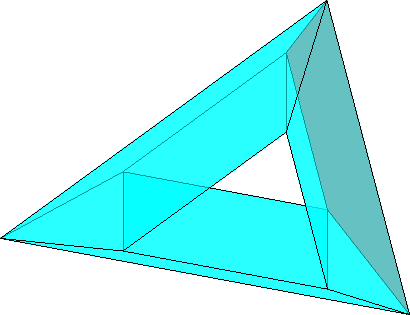
\includegraphics[width=5cm]{Pictures/NURBS/tikz/control_mesh.pdf}};
        
        \node at (3.5,3.5) [inner sep=0pt, scale = 0.5](N2)
        			{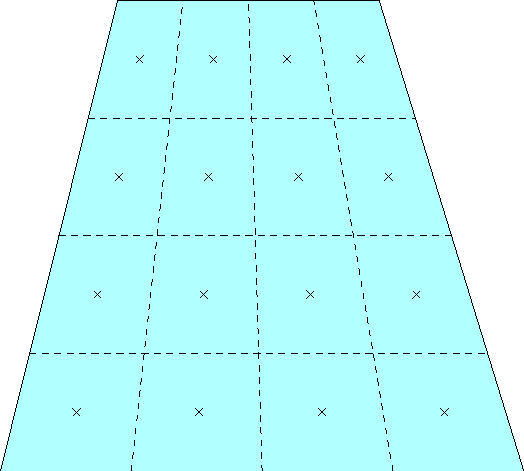
\includegraphics[width=5cm]{Pictures/NURBS/tikz/patch_points.pdf}};
        			                  
        \draw[thick,->] (N1) -- (N2);
        
        
        \node at (7,2)[inner sep=0pt, scale = 0.5](N3)
                  {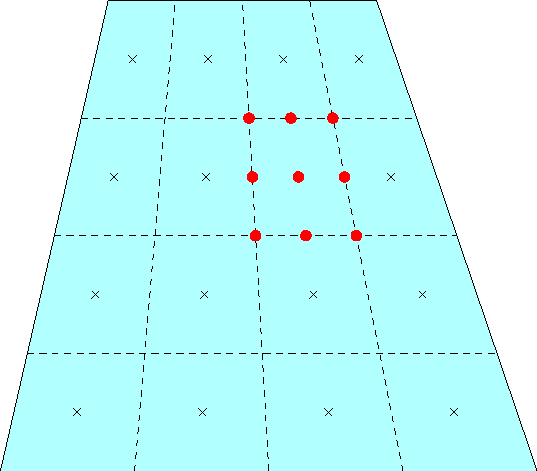
\includegraphics[width=5cm]{Pictures/NURBS/tikz/bezier_points.pdf}};
        \draw[thick,->] (N2) -- (N3);
        
        
        \node at (3.5, 0)[inner sep=0pt, scale = 0.5](N4)
                {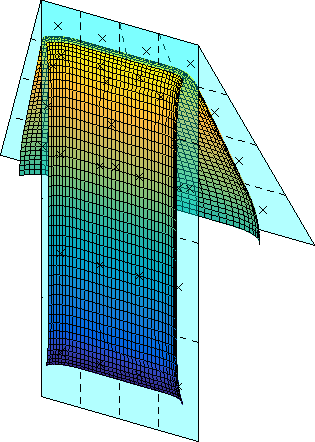
\includegraphics[width=5cm]{Pictures/NURBS/tikz/bspline_patches.pdf}};
        \draw[thick,->] (N3) -- (N4);
        
        
        \node at (0, 0)[inner sep=0pt, scale = 0.5](N5)
                 {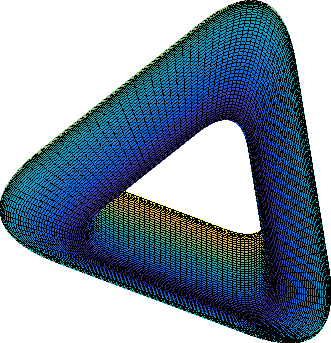
\includegraphics{Pictures/NURBS/tikz/torus_peters.pdf}};
        \draw[thick,->] (N4) -- (N5);
        
        \end{tikzpicture}
	\end{center}
\end{overlayarea}
%\textbf{{\color{red} According to Peters obtained surface is $G^{1}$ smooth}}
\end{frame}

\begin{frame}{Fitting Problem: Peters’ Scheme}
\vspace{-0.5cm}
\only<1>{
\begin{minipage}[t]{0.4\linewidth}
\begin{figure}
	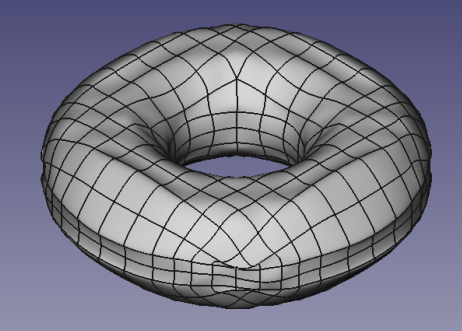
\includegraphics[width=.88\textwidth]{Pictures/NURBS/Torus_wiggly}
\end{figure}
\end{minipage}%
\hfill%
\begin{minipage}[t]{0.55\linewidth}
%\begin{block}{}
\vspace{0.27cm}
\begin{equation*}
||D - C(u, v) \ P||^2  \rightarrow min %\sum_{i=1}^{N}\norm{P_{i} - y_{i}V_{x}}^{2} \rightarrow min$$
\end{equation*}
%\end{block}
\end{minipage}}

\only<2>{
\begin{minipage}[t]{0.4\linewidth}
\begin{figure}
	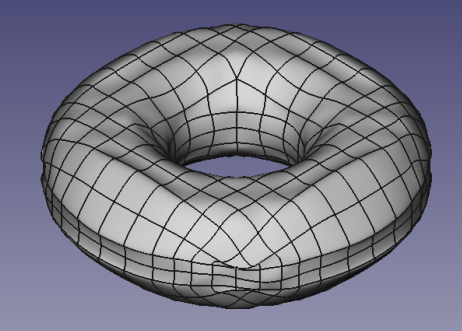
\includegraphics[width=.88\textwidth]{Pictures/NURBS/Torus_wiggly}
\end{figure}
\end{minipage}%
\hfill%
\begin{minipage}[t]{0.55\linewidth}
%\begin{block}{}
\begin{equation*}
||D - C(u, v) \ P||^2 + \textcolor{red}{\lambda ||0-C^{fair}P||}  \rightarrow min %\sum_{i=1}^{N}\norm{P_{i} - y_{i}V_{x}}^{2} \rightarrow min
\end{equation*}
%\end{block}
\end{minipage}}
\vspace{0.2cm}
\only<1>{
\begin{minipage}[t]{0.4\linewidth}
\begin{figure}
	
\includegraphics[width=.88\textwidth]{Pictures/NURBS/ToCover}
\end{figure}
\end{minipage}%
\hfill%
\begin{minipage}[t]{0.55\linewidth}
\begin{block}{Notation}
$D$ - Data  points object to surface fitting\\
$C(u,v)$ - Control Point Matrix \\
$P$ - B-Spline Control Points \\
\end{block}
\end{minipage}}

\only<2>{
\begin{minipage}[t]{0.4\linewidth}
\begin{figure}
	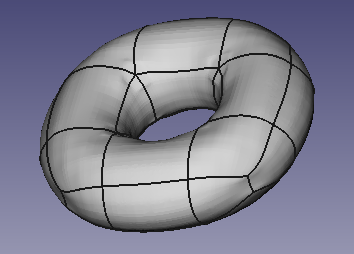
\includegraphics[width=.88\textwidth]{Pictures/NURBS/Torus_smooth}
\end{figure}
\end{minipage}%
\hfill%
\begin{minipage}[t]{0.55\linewidth}
\begin{block}{Notation}
$D$ - Data  points object to surface fitting\\
$C(u,v)$ - Control Point Matrix \\
$P$ - B-Spline Control Points \\
\color{red}{$C^{fair}$ - Fairness coefficients}
\end{block}
\end{minipage}}

\end{frame}

\begin{frame}
Current end
\end{frame}

\begin{frame}{B--Spline}
\begin{equation*}
\vec{S}\left(u,v\right)=\sum\limits_{i,j=1}^{n,m} \vec{C}_{i,j} N_i^p\left(u\right) N_j^p\left(v\right),
\end{equation*}
where $p$ -- degree of the B--Spline surface and $n,m$ -- number of control points in each direction.
\begin{columns}
\begin{column}{.45\textwidth}
B--Splines
\begin{itemize}
\item offer great flexibility for handling arbitrary shapes
\item are CAD--standard
\end{itemize}
\textbf{Engineers are working with CAD}
\end{column}
\begin{column}{.45\textwidth}
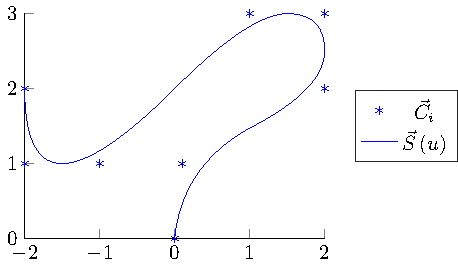
\includegraphics[width=\textwidth]{Pictures/BSplineEx/example.pdf}
\end{column}
\end{columns}
\end{frame}
\begin{frame}{B--Spline Fitting Pipeline [2]}
\begin{figure}
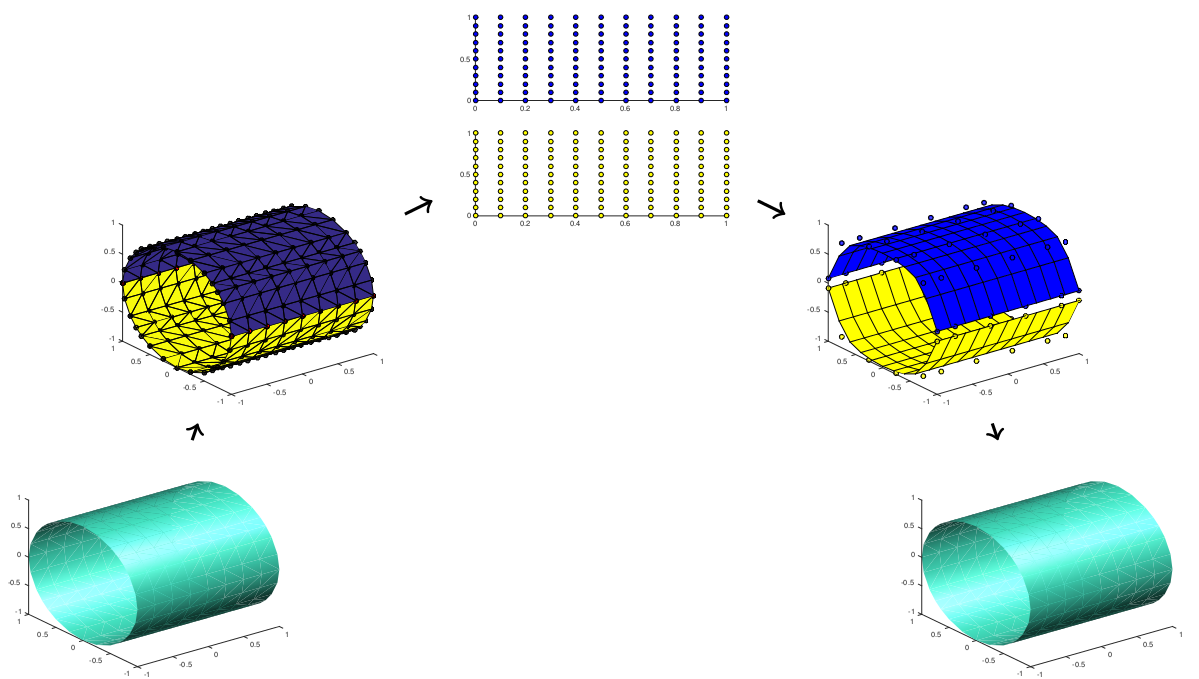
\includegraphics[scale=0.25]{Pictures/NURBS/TheArc.png}
\end{figure}
        
\end{frame}

\begin{frame}{Status}
\begin{block}{Last milestone}
\begin{itemize}
	\item[\textcolor{red}{\XSolidBrush}] Automatic patch selection
	\item[\textcolor{red}{\XSolidBrush}] Parametrization of obtained patches
	\item[\textcolor{green}{\Checkmark}] B--spline fitting using least squares
	\item[\textcolor{black}{\VarClock}] Smooth connection of patches
	\item[\textcolor{red}{\XSolidBrush}] Conversion back to CAD
\end{itemize}
\end{block}
\begin{block}{Today}
\begin{itemize}
	\item[\textcolor{green}{\Checkmark}] Automatic patch selection -- {\color{gray}moved to the surface extraction part}
	\item[\textcolor{green}{\Checkmark}] Parametrization of obtained patches -- {\color{gray}moved to the surface extraction part}
	\item[\textcolor{green}{\Checkmark}] B--spline fitting using least squares --  {\color{gray}modified}
	\item[\textcolor{green}{\Checkmark}] Smooth connection of patches
	\item[\textcolor{red}{\XSolidBrush}] Conversion back to CAD
\end{itemize}
\end{block}
\end{frame}

\begin{frame}{Improved pipeline[3]}
\hspace*{-2cm}%
\begin{tikzpicture} 
        \node at (0,0)[inner sep=0pt, scale = 0.43](N1)
                %{% This file was created by matlab2tikz.
%
%The latest updates can be retrieved from
%  http://www.mathworks.com/matlabcentral/fileexchange/22022-matlab2tikz-matlab2tikz
%where you can also make suggestions and rate matlab2tikz.
%
\definecolor{mycolor1}{rgb}{0.00000,1.00000,1.00000}%
%
\begin{tikzpicture}

\begin{axis}[%
width=4.133in,
height=3.26in,
at={(0.693in,0.44in)},
scale only axis,
xmin=-2,
xmax=3,
tick align=outside,
ymin=-3,
ymax=3,
zmin=-1,
zmax=1,
view={42}{80},
hide axis,
axis x line*=bottom,
axis y line*=left,
axis z line*=left
]

\addplot3[area legend,solid,draw=black,fill=mycolor1,fill opacity=0.3,forget plot]
table[row sep=crcr] {%
x	y	z\\
3	0	0\\
-1.5	2.59807621135332	0\\
-0.75	1.29903810567666	0.866025403784439\\
1.5	0	0.866025403784439\\
}--cycle;

\addplot3[area legend,solid,draw=black,fill=mycolor1,fill opacity=0.3,forget plot]
table[row sep=crcr] {%
x	y	z\\
-1.5	2.59807621135332	0\\
-1.5	-2.59807621135332	0\\
-0.750000000000001	-1.29903810567666	0.866025403784439\\
-0.75	1.29903810567666	0.866025403784439\\
}--cycle;

\addplot3[area legend,solid,draw=black,fill=mycolor1,fill opacity=0.3,forget plot]
table[row sep=crcr] {%
x	y	z\\
-1.5	-2.59807621135332	0\\
3	0	0\\
1.5	0	0.866025403784439\\
-0.750000000000001	-1.29903810567666	0.866025403784439\\
}--cycle;

\addplot3[area legend,solid,draw=black,fill=mycolor1,fill opacity=0.3,forget plot]
table[row sep=crcr] {%
x	y	z\\
1.5	0	0.866025403784439\\
-0.75	1.29903810567666	0.866025403784439\\
-0.749999999999999	1.29903810567666	-0.866025403784438\\
1.5	0	-0.866025403784438\\
}--cycle;

\addplot3[area legend,solid,draw=black,fill=mycolor1,fill opacity=0.3,forget plot]
table[row sep=crcr] {%
x	y	z\\
-0.75	1.29903810567666	0.866025403784439\\
-0.750000000000001	-1.29903810567666	0.866025403784439\\
-0.75	-1.29903810567666	-0.866025403784438\\
-0.749999999999999	1.29903810567666	-0.866025403784438\\
}--cycle;

\addplot3[area legend,solid,draw=black,fill=mycolor1,fill opacity=0.3,forget plot]
table[row sep=crcr] {%
x	y	z\\
-0.750000000000001	-1.29903810567666	0.866025403784439\\
1.5	0	0.866025403784439\\
1.5	0	-0.866025403784438\\
-0.75	-1.29903810567666	-0.866025403784438\\
}--cycle;

\addplot3[area legend,solid,draw=black,fill=mycolor1,fill opacity=0.3,forget plot]
table[row sep=crcr] {%
x	y	z\\
1.5	0	-0.866025403784438\\
-0.749999999999999	1.29903810567666	-0.866025403784438\\
-1.5	2.59807621135332	0\\
3	0	0\\
}--cycle;

\addplot3[area legend,solid,draw=black,fill=mycolor1,fill opacity=0.3,forget plot]
table[row sep=crcr] {%
x	y	z\\
-0.749999999999999	1.29903810567666	-0.866025403784438\\
-0.75	-1.29903810567666	-0.866025403784438\\
-1.5	-2.59807621135332	0\\
-1.5	2.59807621135332	0\\
}--cycle;

\addplot3[area legend,solid,draw=black,fill=mycolor1,fill opacity=0.3,forget plot]
table[row sep=crcr] ;
                {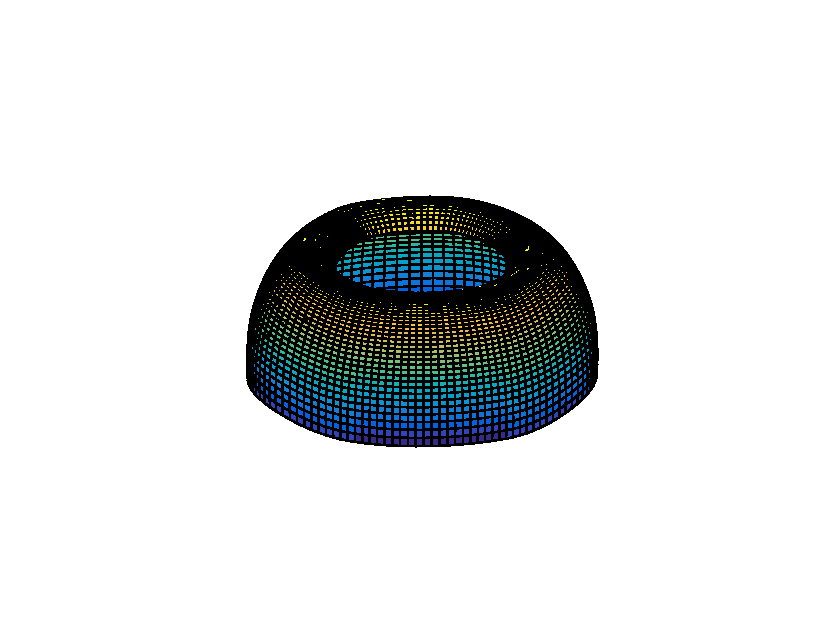
\includegraphics{Pictures/NURBS/fitting_pipeline/half_torus.eps}};
        \node at (2,4) [inner sep=0pt, scale = 0.4](N2)
        			%{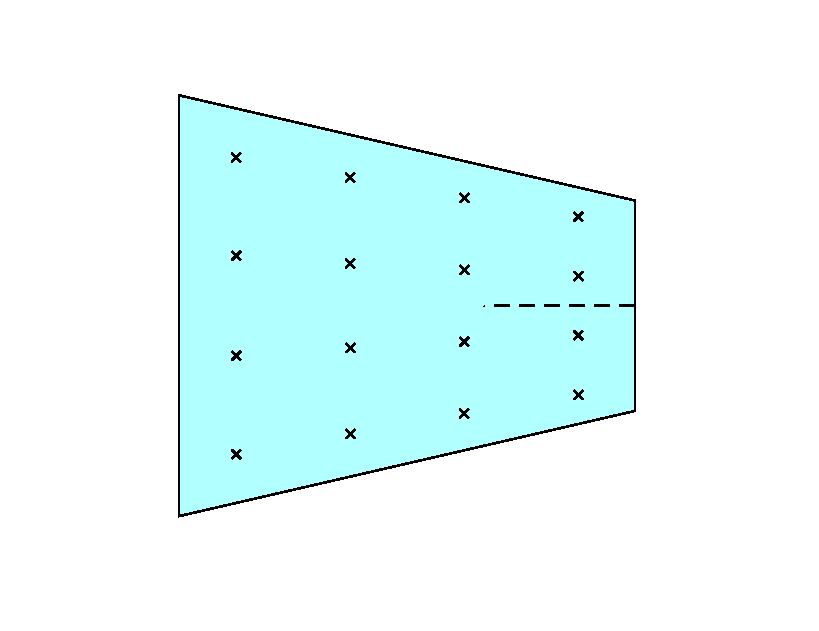
\includegraphics[width=5cm]{Pictures/NURBS/tikz/patch_points.eps}};
                 %{% This file was created by matlab2tikz.
%
%The latest updates can be retrieved from
%  http://www.mathworks.com/matlabcentral/fileexchange/22022-matlab2tikz-matlab2tikz
%where you can also make suggestions and rate matlab2tikz.
%
\definecolor{mycolor1}{rgb}{0.00000,1.00000,1.00000}%
%
\begin{tikzpicture}

\begin{axis}[%
width=4.133in,
height=3.26in,
at={(0.693in,0.44in)},
scale only axis,
xmin=-1.6,
xmax=-0.6,
ymin=-3,
ymax=3,
hide axis,
axis x line*=bottom,
axis y line*=left
]

\addplot[area legend,solid,draw=black,fill=mycolor1,fill opacity=0.3,forget plot]
table[row sep=crcr] {%
x	y\\
-0.749999999999999	1.29903810567666\\
-0.75	-1.29903810567666\\
-1.5	-2.59807621135332\\
-1.5	2.59807621135332\\
}--cycle;
\addplot [color=black,dashed,forget plot]
  table[row sep=crcr]{%
-0.75	0.649519052838329\\
-1.5	1.29903810567666\\
};
\addplot [color=black,dashed,forget plot]
  table[row sep=crcr]{%
-0.937499999999999	1.62379763209582\\
-0.937500000000001	-1.62379763209582\\
};
\addplot [color=black,dashed,forget plot]
  table[row sep=crcr]{%
-0.75	2.22044604925031e-16\\
-1.5	2.22044604925031e-16\\
};
\addplot [color=black,dashed,forget plot]
  table[row sep=crcr]{%
-1.125	1.94855715851499\\
-1.125	-1.94855715851499\\
};
\addplot [color=black,dashed,forget plot]
  table[row sep=crcr]{%
-0.75	-0.649519052838329\\
-1.5	-1.29903810567666\\
};
\addplot [color=black,dashed,forget plot]
  table[row sep=crcr]{%
-1.3125	2.27331668493415\\
-1.3125	-2.27331668493415\\
};
\addplot [color=black,mark size=2.5pt,only marks,mark=x,mark options={solid},forget plot]
  table[row sep=crcr]{%
-0.84375	1.09606340166468\\
};
\addplot [color=black,mark size=2.5pt,only marks,mark=x,mark options={solid},forget plot]
  table[row sep=crcr]{%
-1.03125	1.33963304647905\\
};
\addplot [color=black,mark size=2.5pt,only marks,mark=x,mark options={solid},forget plot]
  table[row sep=crcr]{%
-1.21875	1.58320269129343\\
};
\addplot [color=black,mark size=2.5pt,only marks,mark=x,mark options={solid},forget plot]
  table[row sep=crcr]{%
-1.40625	1.8267723361078\\
};
\addplot [color=black,mark size=2.5pt,only marks,mark=x,mark options={solid},forget plot]
  table[row sep=crcr]{%
-0.84375	0.36535446722156\\
};
\addplot [color=black,mark size=2.5pt,only marks,mark=x,mark options={solid},forget plot]
  table[row sep=crcr]{%
-1.03125	0.446544348826351\\
};
\addplot [color=black,mark size=2.5pt,only marks,mark=x,mark options={solid},forget plot]
  table[row sep=crcr]{%
-1.21875	0.527734230431142\\
};
\addplot [color=black,mark size=2.5pt,only marks,mark=x,mark options={solid},forget plot]
  table[row sep=crcr]{%
-1.40625	0.608924112035934\\
};
\addplot [color=black,mark size=2.5pt,only marks,mark=x,mark options={solid},forget plot]
  table[row sep=crcr]{%
-0.84375	-0.36535446722156\\
};
\addplot [color=black,mark size=2.5pt,only marks,mark=x,mark options={solid},forget plot]
  table[row sep=crcr]{%
-1.03125	-0.446544348826351\\
};
\addplot [color=black,mark size=2.5pt,only marks,mark=x,mark options={solid},forget plot]
  table[row sep=crcr]{%
-1.21875	-0.527734230431142\\
};
\addplot [color=black,mark size=2.5pt,only marks,mark=x,mark options={solid},forget plot]
  table[row sep=crcr]{%
-1.40625	-0.608924112035933\\
};
\addplot [color=black,mark size=2.5pt,only marks,mark=x,mark options={solid},forget plot]
  table[row sep=crcr]{%
-0.84375	-1.09606340166468\\
};
\addplot [color=black,mark size=2.5pt,only marks,mark=x,mark options={solid},forget plot]
  table[row sep=crcr]{%
-1.03125	-1.33963304647905\\
};
\addplot [color=black,mark size=2.5pt,only marks,mark=x,mark options={solid},forget plot]
  table[row sep=crcr]{%
-1.21875	-1.58320269129343\\
};
\addplot [color=black,mark size=2.5pt,only marks,mark=x,mark options={solid},forget plot]
  table[row sep=crcr];
                 {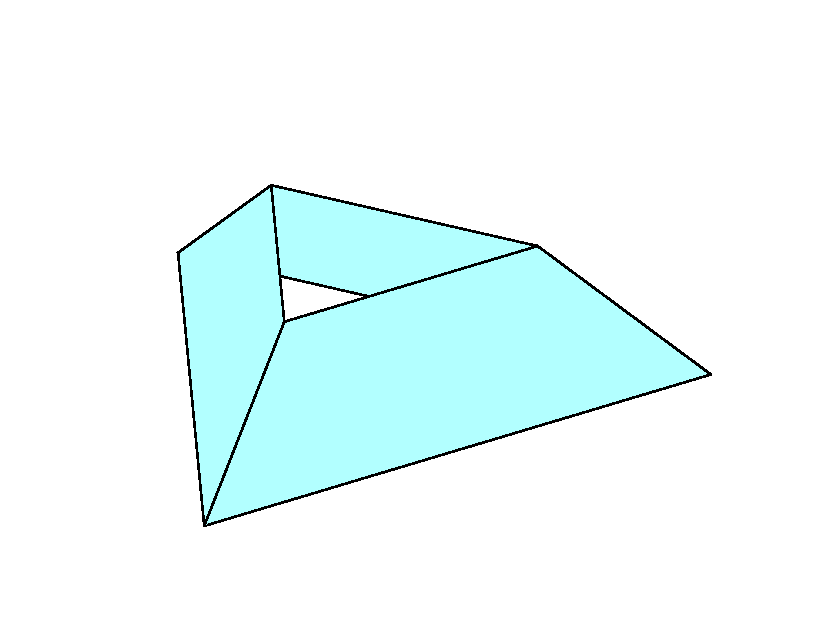
\includegraphics{Pictures/NURBS/fitting_pipeline/half_torus_dc.eps}};                   
        \node at (7,4)[inner sep=0pt, scale = 0.4](N3)
                 %{\documentclass{standalone}
\usepackage{tikz}
\usepackage{pgfplots}
\usepackage{amsmath}
\usepackage{amssymb}
\usepackage{calc}
%-------------------------------------------------------------
% some peters' nomenclature ----------------------------------
\renewcommand{\vec}[1]{\mathbf{#1}}
\newcommand{\petersPatchPoint}{V}
\newcommand{\petersPatchPoints}{\petersPatchPoint_x}
\newcommand{\petersControlMesh}{M}
\newcommand{\petersControlMeshRef}{\petersControlMesh_{ref}}
\newcommand{\petersControlMeshDobRef}{\petersControlMesh_{2ref}}
\newcommand{\petersControlMeshVec}{\vec{\MakeLowercase{\petersControlMesh}}}
\newcommand{\petersPatchPointVec}{\vec{\MakeLowercase{\petersPatchPoint}}}
\newcommand{\petersPatchPointMatrix}{\MakeUppercase{\petersPatchPoint}}
\newcommand{\petersLocalPatchPointLetter}{B}
\newcommand{\petersLocalPatchPoint}{\vec{\petersLocalPatchPointLetter}^{\petersControlMesh}}
\newcommand{\petersLocalPatchPointIndices}[1]{\petersLocalPatchPoint_{#1}}
\newcommand{\petersControlPointCoefLetter}{c}
\newcommand{\petersControlPointCoef}{\petersControlPointCoefLetter^{PS}}
\newcommand{\petersControlPointCoefMatrix}{\MakeUppercase{\petersControlPointCoefLetter}^{PS}}
\newcommand{\bezierPoint}{P}
\newcommand{\bezierPointSet}{\bezierPoint_x}
\newcommand{\bezierPointVec}{\vec{\bezierPoint}}
\newcommand{\petersLocalBezPoint}{\vec{\petersLocalPatchPointLetter}^{\text{B{\'e}z}}}
\newcommand{\petersLocalBezPointIndices}[1]{\petersLocalBezPoint_{#1}}
\newcommand{\petersFaces}{F}
\newcommand{\suchthat}{;}
\newcommand{\centroidof}[1]{\vec{c}_{#1}}
\newcommand{\verticesof}[1]{V_{#1}}
\newcommand{\facesof}[1]{\petersFaces_{#1}}
\newcommand{\lsDataPointLetter}{D}
\newcommand{\lsDataPoint}{\vec{\MakeLowercase{\lsDataPointLetter}}}
\newcommand{\lsDataPointMatrix}{\MakeUppercase{\lsDataPointLetter}}
\newcommand{\lsControlPointLetter}{P}
\newcommand{\lsControlPointMatrix}{\MakeUppercase{\lsControlPointLetter}}
\newcommand{\lsControlPoint}{\vec{\MakeLowercase{\lsControlPointLetter}}}
\newcommand{\lsControlPointCoef}{c}
\newcommand{\lsControlPointCoefVec}{\vec{\lsControlPointCoef}}
\newcommand{\lsControlPointCoefMatrix}{\MakeUppercase{\lsControlPointCoef}}

\newcommand{\lsDataPointi}[1]{\lsDataPoint_{#1}}
\newcommand{\lsControlPointi}[1]{\lsControlPoint_{#1}}
\newcommand{\lsControlPointCoefi}[1]{\lsControlPointCoef_{#1}}


\newcommand{\Bez}{B{\'e}zier }
%-------------------------------------------------------------
% some abreviations ------------------------------------------
\newcommand{\Reg}{$^{\textregistered}$}
\newcommand{\reg}{$^{\textregistered}$ }
\newcommand{\Tm}{\texttrademark}
\newcommand{\tm}{\texttrademark~}
\newcommand {\bsl} {$\backslash$}

\begin{document}

% This file was created by matlab2tikz.
%
%The latest updates can be retrieved from
%  http://www.mathworks.com/matlabcentral/fileexchange/22022-matlab2tikz-matlab2tikz
%where you can also make suggestions and rate matlab2tikz.
%
\definecolor{mycolor1}{rgb}{0.00000,0.7,0.93}%
\definecolor{localmeshcolor}{rgb}{.3,.6,.1}
\definecolor{localbeziercolor}{rgb}{1.0,0.0,0.0}
%
\begin{tikzpicture}

\begin{axis}[%
anchor=origin, % Shift the axis so its origin is at (0,0)
rotate around={90:(current axis.origin)}, % Rotate around the origin
width=4.214in,
height=3.277in,
at={(0.707in,0.442in)},
scale only axis,
xmin=-1.6,
xmax=-0.6,
ymin=-3,
ymax=3,
hide axis,
axis x line*=bottom,
axis y line*=left
]

\addplot[area legend, solid, draw=black, fill=mycolor1, fill opacity=0.2, forget plot]
table[row sep=crcr] {%
x	y\\
-0.749999999999999	1.29903810567666\\
-0.75	-1.29903810567666\\
-1.5	-2.59807621135332\\
-1.5	2.59807621135332\\
}--cycle;
\addplot[area legend, solid, draw=red, thick, fill=mycolor1, fill opacity=0.5, forget plot]
table[row sep=crcr] {%
x	y\\
-1.125	1.94289029309402e-16\\
-1.3125	2.22044604925031e-16\\
-1.3125	-1.13665834246708\\
-1.125	-0.974278579257493\\
}--cycle;
\addplot [color=black,dashed,forget plot]
  table[row sep=crcr]{%
-0.75	0.649519052838329\\
-1.5	1.29903810567666\\
};
\addplot [color=black,dashed,forget plot]
  table[row sep=crcr]{%
-0.937499999999999	1.62379763209582\\
-0.937500000000001	-1.62379763209582\\
};
\addplot [color=black,dashed,forget plot]
  table[row sep=crcr]{%
-0.75	2.22044604925031e-16\\
-1.5	2.22044604925031e-16\\
};
\addplot [color=black,dashed,forget plot]
  table[row sep=crcr]{%
-1.125	1.94855715851499\\
-1.125	-1.94855715851499\\
};
\addplot [color=black,dashed,forget plot]
  table[row sep=crcr]{%
-0.75	-0.649519052838329\\
-1.5	-1.29903810567666\\
};
\addplot [color=black,dashed,forget plot]
  table[row sep=crcr]{%
-1.3125	2.27331668493415\\
-1.3125	-2.27331668493415\\
};
\addplot [color=black,mark size=2.5pt,only marks,mark=x,mark options={solid},forget plot]
  table[row sep=crcr]{%
-0.84375	1.09606340166468\\
};
\addplot [color=black,mark size=2.5pt,only marks,mark=x,mark options={solid},forget plot]
  table[row sep=crcr]{%
-1.03125	1.33963304647905\\
};
\addplot [color=black,mark size=2.5pt,only marks,mark=x,mark options={solid},forget plot]
  table[row sep=crcr]{%
-1.21875	1.58320269129343\\
};
\addplot [color=black,mark size=2.5pt,only marks,mark=x,mark options={solid},forget plot]
  table[row sep=crcr]{%
-1.40625	1.8267723361078\\
};
\addplot [color=black,mark size=2.5pt,only marks,mark=x,mark options={solid},forget plot]
  table[row sep=crcr]{%
-0.84375	0.36535446722156\\
};
\addplot [color=localmeshcolor,mark size=2.5pt,only marks,mark=x,mark options={solid},forget plot]
  table[row sep=crcr]{%
-1.03125	0.446544348826351\\
};
\addplot [color=localmeshcolor,mark size=2.5pt,only marks,mark=x,mark options={solid},forget plot]
  table[row sep=crcr]{%
-1.21875	0.527734230431142\\
};
\addplot [color=localmeshcolor,mark size=2.5pt,only marks,mark=x,mark options={solid},forget plot]
  table[row sep=crcr]{%
-1.40625	0.608924112035934\\
};
\addplot [color=black,mark size=2.5pt,only marks,mark=x,mark options={solid},forget plot]
  table[row sep=crcr]{%
-0.84375	-0.36535446722156\\
};
\addplot [color=localmeshcolor,mark size=2.5pt,only marks,mark=x,mark options={solid},forget plot]
  table[row sep=crcr]{%
-1.03125	-0.446544348826351\\
};
\addplot [color=localmeshcolor,mark size=2.5pt,only marks,mark=x,mark options={solid},forget plot]
  table[row sep=crcr]{%
-1.21875	-0.527734230431142\\
};
\addplot [color=localmeshcolor,mark size=2.5pt,only marks,mark=x,mark options={solid},forget plot]
  table[row sep=crcr]{%
-1.40625	-0.608924112035933\\
};
\addplot [color=black,mark size=2.5pt,only marks,mark=x,mark options={solid},forget plot]
  table[row sep=crcr]{%
-0.84375	-1.09606340166468\\
};
\addplot [color=localmeshcolor,mark size=2.5pt,only marks,mark=x,mark options={solid},forget plot]
  table[row sep=crcr]{%
-1.03125	-1.33963304647905\\
};
\addplot [color=localmeshcolor,mark size=2.5pt,only marks,mark=x,mark options={solid},forget plot]
  table[row sep=crcr]{%
-1.21875	-1.58320269129343\\
};
\addplot [color=localmeshcolor,mark size=2.5pt,only marks,mark=x,mark options={solid},forget plot]
  table[row sep=crcr]{%
-1.40625	-1.8267723361078\\
};
\addplot[only marks,mark=o,color=localbeziercolor,mark options={},mark size=2.5000pt] plot table[row sep=crcr]{%
-1.125	1.94289029309402e-16\\
-1.21875	1.66533453693773e-16\\
-1.3125	2.22044604925031e-16\\
-1.125	-0.487139289628746\\
-1.21875	-0.527734230431142\\
-1.3125	-0.568329171233538\\
-1.125	-0.974278579257493\\
-1.21875	-1.05546846086228\\
-1.3125	-1.13665834246708\\
};

\tikzstyle{dot}=[draw,shape=circle, inner sep = 2pt, outer sep = -2pt]
\tikzstyle{localbezier}=[inner sep = 2pt, outer sep = -2pt]
\tikzstyle{localmesh}=[inner sep = 2pt, outer sep = -2pt]
\tikzstyle{meshdot}=[dot, fill=black]

\node[meshdot, label={above left:D}] at (axis cs:-0.74999999999999,1.29903810567666){};
\node[meshdot, label={above right:C}] at (axis cs: -0.75,	-1.29903810567666){};
\node[meshdot, label={below right:B}] at (axis cs:-1.5,	-2.59807621135332){};
\node[meshdot, label={below left:A}] at (axis cs:-1.5,	2.59807621135332){};

\node[localbezier,label={[localbeziercolor]above left:$\petersLocalBezPointIndices{-1,1}$}] at (axis cs:-1.125, 1.94289029309402e-16){};
\node[localbezier,label={[localbeziercolor]above left:$\petersLocalBezPointIndices{-1,0}$}] at (axis cs:-1.21875, 1.66533453693773e-16){};
\node[localbezier,label={[localbeziercolor]below left:$\petersLocalBezPointIndices{-1,-1}$}] at (axis cs:
-1.3125,2.22044604925031e-16){};
\node[localbezier,label={[localbeziercolor]above:$\petersLocalBezPointIndices{0,1}$}] at (axis cs:-1.125,-0.487139289628746){};
\node[localbezier,label={[localbeziercolor]$\petersLocalBezPointIndices{0,0}$}] at (axis cs:-1.21875,-0.527734230431142){};
\node[localbezier,label={[localbeziercolor]below:$\petersLocalBezPointIndices{0,-1}$}] at (axis cs:-1.3125,-0.568329171233538){};
\node[localbezier,label={[localbeziercolor]above right:$\petersLocalBezPointIndices{1,1}$}] at (axis cs:-1.125,-0.974278579257493){};
\node[localbezier,label={[localbeziercolor]above right:$\petersLocalBezPointIndices{1,0}$}] at (axis cs:-1.21875,-1.05546846086228){};
\node[localbezier,label={[localbeziercolor]below right:$\petersLocalBezPointIndices{1,-1}$}] at (axis cs:-1.3125,-1.13665834246708){};

\node[localmesh,label={[localmeshcolor]below:$\petersLocalPatchPointIndices{1,0}$}] at (axis cs:-1.21875,	-1.58320269129343){};
\node[localmesh,label={[localmeshcolor]below:$\petersLocalPatchPointIndices{0,-1}$}] at (axis cs:-1.40625, -0.608924112035933){};
\node[localmesh,label={[localmeshcolor]below:$\petersLocalPatchPointIndices{0,0}$}] at (axis cs:-1.21875,	-0.527734230431142){};
\node[localmesh,label={[localmeshcolor]above:$\petersLocalPatchPointIndices{0,1}$}] at (axis cs:-1.03125,	-0.446544348826351){};
\node[localmesh,label={[localmeshcolor]below:$\petersLocalPatchPointIndices{-1,0}$}] at (axis cs:-1.21875,	0.527734230431142){};
\node[localmesh,label={[localmeshcolor]above:$\petersLocalPatchPointIndices{-1,1}$}] at (axis cs:-1.03125,	0.446544348826351){};
\node[localmesh,label={[localmeshcolor]below:$\petersLocalPatchPointIndices{-1,-1}$}] at (axis cs:-1.40625,	0.608924112035934){};
\node[localmesh,label={[localmeshcolor]above:$\petersLocalPatchPointIndices{1,1}$}] at (axis cs:-1.03125,	-1.33963304647905){};
\node[localmesh,label={[localmeshcolor]below:$\petersLocalPatchPointIndices{1,-1}$}] at (axis cs:-1.40625,	-1.8267723361078){};


\end{axis}

\end{tikzpicture}%

\end{document}};
                  %{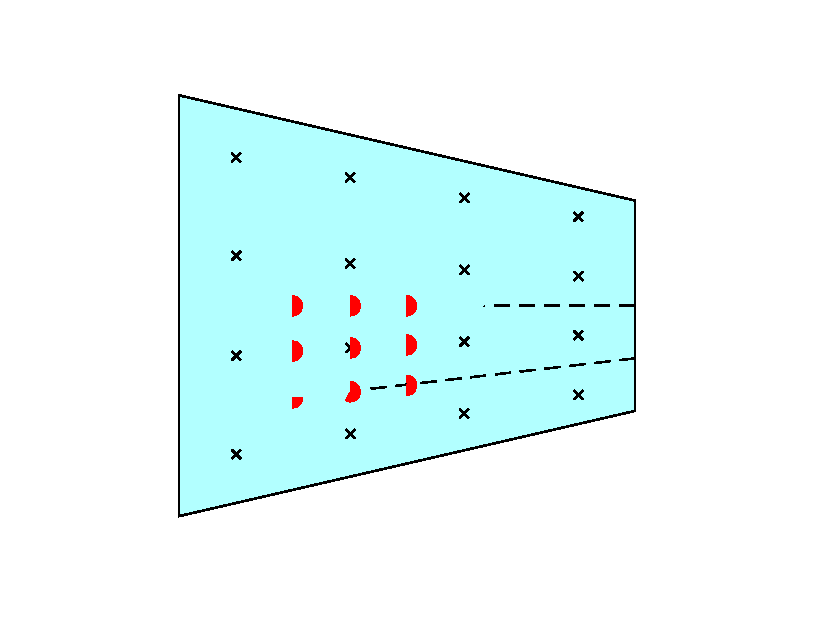
\includegraphics[width=5cm]{Pictures/NURBS/tikz/bezier_points.eps}};
                  {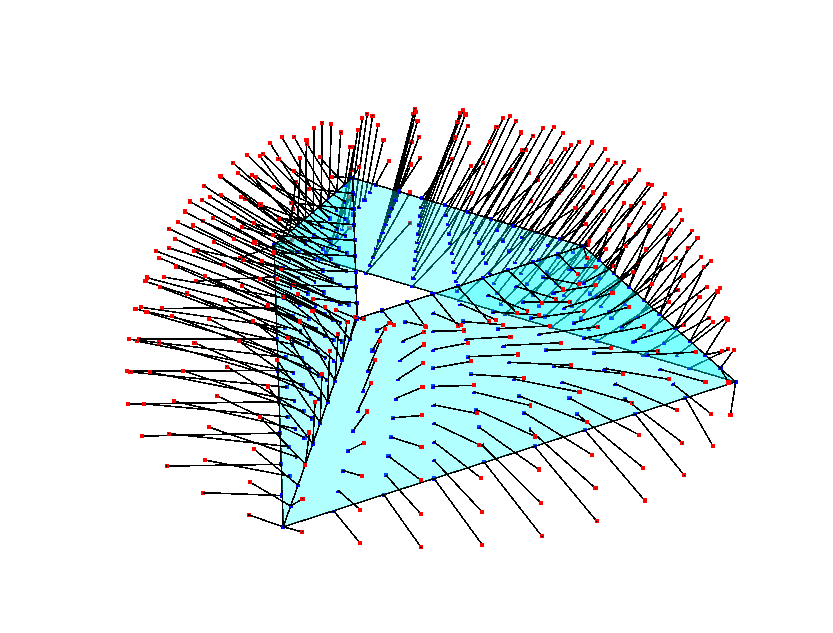
\includegraphics{Pictures/NURBS/fitting_pipeline/half_torus_hair.eps}};        
        \node at (9, 0)[inner sep=0pt, scale = 0.43](N4)
                 %{% This file was created by matlab2tikz.
%
%The latest updates can be retrieved from
%  http://www.mathworks.com/matlabcentral/fileexchange/22022-matlab2tikz-matlab2tikz
%where you can also make suggestions and rate matlab2tikz.
%
\definecolor{mycolor1}{rgb}{0.00000,1.00000,1.00000}%
%
\begin{tikzpicture}

\begin{axis}[%
width=4.133in,
height=3.26in,
at={(0.693in,0.44in)},
scale only axis,
xmin=-2,
xmax=4,
tick align=outside,
ymin=-1,
ymax=4,
zmin=-0.2,
zmax=1.2,
view={-102}{28},
hide axis,
axis x line*=bottom,
axis y line*=left,
axis z line*=left
]

\addplot3[%
surf,
shader=flat corner,draw=black,z buffer=sort,colormap={mymap}{[1pt] rgb(0pt)=(0.2081,0.1663,0.5292); rgb(1pt)=(0.211624,0.189781,0.577676); rgb(2pt)=(0.212252,0.213771,0.626971); rgb(3pt)=(0.2081,0.2386,0.677086); rgb(4pt)=(0.195905,0.264457,0.7279); rgb(5pt)=(0.170729,0.291938,0.779248); rgb(6pt)=(0.125271,0.324243,0.830271); rgb(7pt)=(0.0591333,0.359833,0.868333); rgb(8pt)=(0.0116952,0.38751,0.881957); rgb(9pt)=(0.00595714,0.408614,0.882843); rgb(10pt)=(0.0165143,0.4266,0.878633); rgb(11pt)=(0.0328524,0.443043,0.871957); rgb(12pt)=(0.0498143,0.458571,0.864057); rgb(13pt)=(0.0629333,0.47369,0.855438); rgb(14pt)=(0.0722667,0.488667,0.8467); rgb(15pt)=(0.0779429,0.503986,0.838371); rgb(16pt)=(0.0793476,0.520024,0.831181); rgb(17pt)=(0.0749429,0.537543,0.826271); rgb(18pt)=(0.0640571,0.556986,0.823957); rgb(19pt)=(0.0487714,0.577224,0.822829); rgb(20pt)=(0.0343429,0.596581,0.819852); rgb(21pt)=(0.0265,0.6137,0.8135); rgb(22pt)=(0.0238905,0.628662,0.803762); rgb(23pt)=(0.0230905,0.641786,0.791267); rgb(24pt)=(0.0227714,0.653486,0.776757); rgb(25pt)=(0.0266619,0.664195,0.760719); rgb(26pt)=(0.0383714,0.674271,0.743552); rgb(27pt)=(0.0589714,0.683757,0.725386); rgb(28pt)=(0.0843,0.692833,0.706167); rgb(29pt)=(0.113295,0.7015,0.685857); rgb(30pt)=(0.145271,0.709757,0.664629); rgb(31pt)=(0.180133,0.717657,0.642433); rgb(32pt)=(0.217829,0.725043,0.619262); rgb(33pt)=(0.258643,0.731714,0.595429); rgb(34pt)=(0.302171,0.737605,0.571186); rgb(35pt)=(0.348167,0.742433,0.547267); rgb(36pt)=(0.395257,0.7459,0.524443); rgb(37pt)=(0.44201,0.748081,0.503314); rgb(38pt)=(0.487124,0.749062,0.483976); rgb(39pt)=(0.530029,0.749114,0.466114); rgb(40pt)=(0.570857,0.748519,0.44939); rgb(41pt)=(0.609852,0.747314,0.433686); rgb(42pt)=(0.6473,0.7456,0.4188); rgb(43pt)=(0.683419,0.743476,0.404433); rgb(44pt)=(0.71841,0.741133,0.390476); rgb(45pt)=(0.752486,0.7384,0.376814); rgb(46pt)=(0.785843,0.735567,0.363271); rgb(47pt)=(0.818505,0.732733,0.34979); rgb(48pt)=(0.850657,0.7299,0.336029); rgb(49pt)=(0.882433,0.727433,0.3217); rgb(50pt)=(0.913933,0.725786,0.306276); rgb(51pt)=(0.944957,0.726114,0.288643); rgb(52pt)=(0.973895,0.731395,0.266648); rgb(53pt)=(0.993771,0.745457,0.240348); rgb(54pt)=(0.999043,0.765314,0.216414); rgb(55pt)=(0.995533,0.786057,0.196652); rgb(56pt)=(0.988,0.8066,0.179367); rgb(57pt)=(0.978857,0.827143,0.163314); rgb(58pt)=(0.9697,0.848138,0.147452); rgb(59pt)=(0.962586,0.870514,0.1309); rgb(60pt)=(0.958871,0.8949,0.113243); rgb(61pt)=(0.959824,0.921833,0.0948381); rgb(62pt)=(0.9661,0.951443,0.0755333); rgb(63pt)=(0.9763,0.9831,0.0538)},mesh/rows=11]
table[row sep=crcr, point meta=\thisrow{c}] {%
%
x	y	z	c\\
2.53381548064847	1.42472903318201	0.494640048011155	0.494640048011155\\
2.55647171669891	1.43743759838618	0.450306097153373	0.450306097153373\\
2.5760658107946	1.44842736585171	0.402747550860707	0.402747550860707\\
2.59259776293553	1.45769833557862	0.351964409133158	0.351964409133158\\
2.6060675731217	1.46525050756689	0.297956671970726	0.297956671970726\\
2.61647524135311	1.47108388181652	0.240724339373411	0.240724339373411\\
2.62382076762977	1.47519845832752	0.180267411341212	0.180267411341212\\
2.62810415195166	1.47759423709989	0.116585887874131	0.116585887874131\\
2.6293253943188	1.47827121813363	0.0496797689721661	0.0496797689721661\\
2.62748449473118	1.47722940142873	-0.0204509453646816	-0.0204509453646816\\
2.6225814531888	1.4744687869852	-0.0938062551364125	-0.0938062551364125\\
2.60799867965941	1.29711929567782	0.49462837395119	0.49462837395119\\
2.63131892464297	1.30866945023801	0.45029025590804	0.45029025590804\\
2.65148651514488	1.31865037099328	0.402728944250207	0.402728944250207\\
2.6685017306989	1.32706496884325	0.35194436412444	0.35194436412444\\
2.68236485083884	1.3339161546875	0.297936440677486	0.297936440677486\\
2.69307615509846	1.33920683942565	0.24070509905609	0.24070509905609\\
2.70063592301154	1.34293993395729	0.180250264407001	0.180250264407001\\
2.70504443411186	1.34511834918203	0.116571861876965	0.116571861876965\\
2.7063019679332	1.34574499599947	0.0496698166127295	0.0496698166127295\\
2.70440880400934	1.34482278530922	-0.0204559462389592	-0.0204559462389592\\
2.69936522187406	1.34235462801087	-0.0938055015313538	-0.0938055015313538\\
2.67215374597365	1.16020382886545	0.494620238037823	0.494620238037823\\
2.69604771043771	1.1705091631769	0.450279424151137	0.450279424151137\\
2.71670959925503	1.17939494449834	0.402716718316971	0.402716718316971\\
2.73414040632349	1.18687152269503	0.351931854390423	0.351931854390423\\
2.74834112554096	1.19294924763221	0.297924566226596	0.297924566226596\\
2.75931275080534	1.19763846917514	0.240694587680588	0.240694587680588\\
2.7670562760145	1.20094953718907	0.180241652607501	0.180241652607501\\
2.77157269506633	1.20289280153927	0.116565494862433	0.116565494862433\\
2.7728630018587	1.20347861209097	0.0496658483004869	0.0496658483004869\\
2.77092819028949	1.20271731870944	-0.0204575532232385	-0.0204575532232385\\
2.7657692542566	1.20061927125993	-0.0938049758536427	-0.0938049758536427\\
2.72628067959119	1.01398263274492	0.494615640271052	0.494615640271052\\
2.75065835361692	1.02295964810247	0.450273527029412	0.450273527029412\\
2.77173605702294	1.03067143623214	0.402710606916097	0.402710606916097\\
2.78951574654572	1.03713837343117	0.351926355958336	0.351926355958336\\
2.80399937892171	1.04238083599676	0.297920250183357	0.297920250183357\\
2.81518891088736	1.04641920022613	0.240691765618389	0.240691765618389\\
2.82308629917912	1.04927384241651	0.180240378290661	0.180240378290661\\
2.82769350053346	1.0509651388651	0.116565564227402	0.116565564227402\\
2.82901247168681	1.05151346586913	0.0496667994558394	0.0496667994558394\\
2.82704516937564	1.05093919972581	-0.020456439996797	-0.020456439996797\\
2.8217935503364	1.04926271673236	-0.093804678103279	-0.093804678103279\\
2.77037948051203	0.858455707316207	0.494614580650879	0.494614580650879\\
2.79515113371437	0.866023815914299	0.450272489689612	0.450272489689612\\
2.8165668823465	0.872490196059942	0.402710343902687	0.402710343902687\\
2.83462970810207	0.877885897348897	0.351927344855406	0.351927344855406\\
2.84934259267473	0.882241969376924	0.29792269411307	0.29792269411307\\
2.86070851775812	0.885589461739784	0.240695593240979	0.240695593240979\\
2.86873046504587	0.887959424033237	0.180245243804435	0.180245243804435\\
2.87341141623164	0.889382905853043	0.116570847368737	0.116570847368737\\
2.87475435300907	0.889890956794964	0.0496716054991882	0.0496716054991882\\
2.8727622570718	0.889514626454759	-0.0204532802389121	-0.0204532802389121\\
2.86743811011348	0.888284964428189	-0.0938046082802628	-0.0938046082802628\\
2.80445014873617	0.693623052579323	0.494617059177303	0.494617059177303\\
2.82952633026384	0.699704577512004	0.450276237278482	0.450276237278482\\
2.85120306912358	0.70486157384699	0.40271566313184	0.40271566313184\\
2.86948424772899	0.709134470745426	0.351934297108862	0.351934297108862\\
2.88437374849366	0.712563697368459	0.297931099581035	0.297931099581035\\
2.8958754538312	0.715189682877235	0.240705030919843	0.240705030919843\\
2.90399324615521	0.717052856432902	0.180255051496772	0.180255051496772\\
2.90873100787927	0.718193647196605	0.116580121683307	0.116580121683307\\
2.910092621417	0.718652484329491	0.0496792018509343	0.0496792018509343\\
2.90808196918198	0.718469796992706	-0.0204487476288612	-0.0204487476288612\\
2.90270293358783	0.717686014347397	-0.093804766384594	-0.093804766384594\\
2.8284926842636	0.519484668534266	0.494623075850325	0.494623075850325\\
2.85378422279911	0.524004843795185	0.450284694942771	0.450284694942771\\
2.87564561125206	0.52779591945854	0.402726298458657	0.402726298458657\\
2.89408132216292	0.530904469917973	0.351946688745934	0.351946688745934\\
2.90909582807216	0.533377069567124	0.297944668152554	0.297944668152554\\
2.92069360152023	0.535260292799634	0.240719039026467	0.240719039026467\\
2.9288791150476	0.536600714009143	0.180268603715624	0.180268603715624\\
2.93365684119474	0.537444907589292	0.116592164567978	0.116592164567978\\
2.93503125250212	0.537839447933723	0.0496885239314789	0.0496885239314789\\
2.9330068215102	0.537830909436075	-0.0204435158459217	-0.0204435158459217\\
2.92758802075945	0.537465866489989	-0.0938051524162727	-0.0938051524162727\\
2.84250708709434	0.336040555181036	0.494632630669943	0.494632630669943\\
2.86792509085397	0.338927525663443	0.450297787829225	0.450297787829225\\
2.88989550262983	0.341303582759848	0.402741983738239	0.402741983738239\\
2.90842288814033	0.343216271163757	0.35196399579385	0.35196399579385\\
2.92351181310385	0.34471313556868	0.297962601392927	0.297962601392927\\
2.93516684323878	0.345841720668126	0.240736577932336	0.240736577932336\\
2.94339254426351	0.346649571155601	0.180284702808943	0.180284702808943\\
2.94819348189644	0.347184231724614	0.116605753419617	0.116605753419617\\
2.94957422185596	0.347493247068674	0.049698507161223	0.049698507161223\\
2.94753932986046	0.347624161881288	-0.0204382585693711	-0.0204382585693711\\
2.94209337162833	0.347624520855965	-0.0938057663752988	-0.0938057663752988\\
2.84649335722837	0.143290712519632	0.494645723636159	0.494645723636159\\
2.87194921396218	0.144475534016382	0.450315441084592	0.450315441084592\\
2.89395373715477	0.145394913616165	0.402762452825685	0.402762452825685\\
2.91251090239766	0.146090250779996	0.351985694279839	0.351985694279839\\
2.92762468528238	0.146602944968889	0.297984100867455	0.297984100867455\\
2.93929906140046	0.146974395643857	0.240756608008935	0.240756608008935\\
2.94753800634341	0.147246002265916	0.18030215112468	0.18030215112468\\
2.95234549570276	0.147459164296078	0.11661966563509	0.11661966563509\\
2.95372550507005	0.147655281195357	0.0497080869605678	0.0497080869605678\\
2.95168201003678	0.147875752424769	-0.0204336494784869	-0.0204336494784869\\
2.94621898619449	0.148161977445325	-0.0938066082616724	-0.0938066082616724\\
2.8404514946657	-0.0587648594499441	0.494662354748973	0.494662354748973\\
2.86585687165754	-0.059348220246397	0.450337579855618	0.450337579855618\\
2.88782130872476	-0.0599197381072544	0.402787439576095	0.402787439576095\\
2.90634732167138	-0.0604532149360934	0.352011260231128	0.352011260231128\\
2.92143742630141	-0.0609224526364911	0.298008368141439	0.298008368141439\\
2.93309413841887	-0.0613012531120248	0.240778089627751	0.240778089627751\\
2.94131997382776	-0.0615634182662714	0.180319751010785	0.180319751010785\\
2.9461174483321	-0.0616827500028081	0.116632678611266	0.116632678611266\\
2.9474890777359	-0.0616330502252121	0.0497161987499143	0.0497161987499143\\
2.94543737784317	-0.0613881208370604	-0.0204303622525463	-0.0204303622525463\\
2.93996486445792	-0.06092176374193	-0.0938076780753935	-0.0938076780753935\\
2.82438149940633	-0.270126160727694	0.494682524008383	0.494682524008383\\
2.84964834347381	-0.27254082622529	0.450364129289049	0.450364129289049\\
2.87149921123767	-0.274630022545156	0.402816677844571	0.402816677844571\\
2.88993410269792	-0.276393749687292	0.352040169674948	0.352040169674948\\
2.90495301785457	-0.277832007651698	0.29803460478018	0.29803460478018\\
2.9165559567076	-0.278944796438374	0.240799983160268	0.240799983160268\\
2.92474291925702	-0.27973211604732	0.180336304815211	0.180336304815211\\
2.92951390550284	-0.280193966478535	0.11664356974501	0.11664356974501\\
2.93086891544504	-0.280330347732021	0.0497217779496637	0.0497217779496637\\
2.92880794908364	-0.280141259807776	-0.0204290705708269	-0.0204290705708269\\
2.92333100641862	-0.279626702705801	-0.093808975816462	-0.093808975816462\\
};

\addplot3[%
surf,
shader=flat corner,draw=black,z buffer=sort,colormap={mymap}{[1pt] rgb(0pt)=(0.2081,0.1663,0.5292); rgb(1pt)=(0.211624,0.189781,0.577676); rgb(2pt)=(0.212252,0.213771,0.626971); rgb(3pt)=(0.2081,0.2386,0.677086); rgb(4pt)=(0.195905,0.264457,0.7279); rgb(5pt)=(0.170729,0.291938,0.779248); rgb(6pt)=(0.125271,0.324243,0.830271); rgb(7pt)=(0.0591333,0.359833,0.868333); rgb(8pt)=(0.0116952,0.38751,0.881957); rgb(9pt)=(0.00595714,0.408614,0.882843); rgb(10pt)=(0.0165143,0.4266,0.878633); rgb(11pt)=(0.0328524,0.443043,0.871957); rgb(12pt)=(0.0498143,0.458571,0.864057); rgb(13pt)=(0.0629333,0.47369,0.855438); rgb(14pt)=(0.0722667,0.488667,0.8467); rgb(15pt)=(0.0779429,0.503986,0.838371); rgb(16pt)=(0.0793476,0.520024,0.831181); rgb(17pt)=(0.0749429,0.537543,0.826271); rgb(18pt)=(0.0640571,0.556986,0.823957); rgb(19pt)=(0.0487714,0.577224,0.822829); rgb(20pt)=(0.0343429,0.596581,0.819852); rgb(21pt)=(0.0265,0.6137,0.8135); rgb(22pt)=(0.0238905,0.628662,0.803762); rgb(23pt)=(0.0230905,0.641786,0.791267); rgb(24pt)=(0.0227714,0.653486,0.776757); rgb(25pt)=(0.0266619,0.664195,0.760719); rgb(26pt)=(0.0383714,0.674271,0.743552); rgb(27pt)=(0.0589714,0.683757,0.725386); rgb(28pt)=(0.0843,0.692833,0.706167); rgb(29pt)=(0.113295,0.7015,0.685857); rgb(30pt)=(0.145271,0.709757,0.664629); rgb(31pt)=(0.180133,0.717657,0.642433); rgb(32pt)=(0.217829,0.725043,0.619262); rgb(33pt)=(0.258643,0.731714,0.595429); rgb(34pt)=(0.302171,0.737605,0.571186); rgb(35pt)=(0.348167,0.742433,0.547267); rgb(36pt)=(0.395257,0.7459,0.524443); rgb(37pt)=(0.44201,0.748081,0.503314); rgb(38pt)=(0.487124,0.749062,0.483976); rgb(39pt)=(0.530029,0.749114,0.466114); rgb(40pt)=(0.570857,0.748519,0.44939); rgb(41pt)=(0.609852,0.747314,0.433686); rgb(42pt)=(0.6473,0.7456,0.4188); rgb(43pt)=(0.683419,0.743476,0.404433); rgb(44pt)=(0.71841,0.741133,0.390476); rgb(45pt)=(0.752486,0.7384,0.376814); rgb(46pt)=(0.785843,0.735567,0.363271); rgb(47pt)=(0.818505,0.732733,0.34979); rgb(48pt)=(0.850657,0.7299,0.336029); rgb(49pt)=(0.882433,0.727433,0.3217); rgb(50pt)=(0.913933,0.725786,0.306276); rgb(51pt)=(0.944957,0.726114,0.288643); rgb(52pt)=(0.973895,0.731395,0.266648); rgb(53pt)=(0.993771,0.745457,0.240348); rgb(54pt)=(0.999043,0.765314,0.216414); rgb(55pt)=(0.995533,0.786057,0.196652); rgb(56pt)=(0.988,0.8066,0.179367); rgb(57pt)=(0.978857,0.827143,0.163314); rgb(58pt)=(0.9697,0.848138,0.147452); rgb(59pt)=(0.962586,0.870514,0.1309); rgb(60pt)=(0.958871,0.8949,0.113243); rgb(61pt)=(0.959824,0.921833,0.0948381); rgb(62pt)=(0.9661,0.951443,0.0755333); rgb(63pt)=(0.9763,0.9831,0.0538)},mesh/rows=11]
table[row sep=crcr, point meta=\thisrow{c}] {%
%
x	y	z	c\\
2.6225814531888	1.4744687869852	-0.0938062551364125	-0.0938062551364125\\
2.62748449473118	1.47722940142873	-0.0204509453646816	-0.0204509453646816\\
2.6293253943188	1.47827121813363	0.0496797689721662	0.0496797689721662\\
2.62810415195166	1.47759423709989	0.116585887874131	0.116585887874131\\
2.62382076762977	1.47519845832752	0.180267411341212	0.180267411341212\\
2.61647524135311	1.47108388181652	0.240724339373411	0.240724339373411\\
2.6060675731217	1.46525050756689	0.297956671970726	0.297956671970726\\
2.59259776293553	1.45769833557862	0.351964409133158	0.351964409133158\\
2.5760658107946	1.44842736585171	0.402747550860707	0.402747550860707\\
2.55647171669891	1.43743759838618	0.450306097153373	0.450306097153373\\
2.53381548064847	1.42472903318201	0.494640048011155	0.494640048011155\\
2.53824686864102	1.59943348695382	-0.0938070793267082	-0.0938070793267082\\
2.54299175846195	1.60243415808068	-0.0204443691045975	-0.0204443691045975\\
2.54477311829597	1.60356789608836	0.0496924032529211	0.0496924032529211\\
2.54359094814309	1.60283470097687	0.116603237745848	0.116603237745848\\
2.5394452480033	1.6002345727462	0.180288134374182	0.180288134374182\\
2.53233601787661	1.59576751139635	0.240747093137925	0.240747093137925\\
2.52226325776302	1.58943351692733	0.297980114037075	0.297980114037075\\
2.50922696766252	1.58123258933913	0.351987197071633	0.351987197071633\\
2.49322714757512	1.57116472863176	0.402768342241599	0.402768342241599\\
2.47426379750081	1.55922993480521	0.450323549546974	0.450323549546974\\
2.4523369174396	1.54542820785948	0.494652818987756	0.494652818987756\\
2.44919038867096	1.71972046668765	-0.0938078167601307	-0.0938078167601307\\
2.45376876841128	1.72295151167539	-0.020438485082417	-0.020438485082417\\
2.45548762753954	1.72417324709928	0.049703707609386	0.049703707609386\\
2.45434696605575	1.72338567295932	0.116618761315279	0.116618761315279\\
2.45034678395989	1.7205887892555	0.18030667603526	0.18030667603526\\
2.44348708125198	1.71578259598784	0.240767451769332	0.240767451769332\\
2.43376785793202	1.70896709315631	0.298001088517493	0.298001088517493\\
2.421189114	1.70014228076094	0.352007586279743	0.352007586279743\\
2.40575084945592	1.68930815880171	0.402786945056082	0.402786945056082\\
2.38745306429978	1.67646472727863	0.450339164846511	0.450339164846511\\
2.36629575853159	1.6616119861917	0.49466424565103	0.49466424565103\\
2.3554120132786	1.83532972618668	-0.0938084674366799	-0.0938084674366799\\
2.35981552457916	1.83878146221287	-0.0204332932981401	-0.0204332932981401\\
2.36146892204951	1.84008727116639	0.049713682041561	0.049713682041561\\
2.36037220568964	1.83924715304725	0.116632458582423	0.116632458582423\\
2.35652537549955	1.83626110785544	0.180323036324447	0.180323036324447\\
2.34992843147924	1.83112913559097	0.240785415267632	0.240785415267632\\
2.34058137362871	1.82385123625384	0.298019595411979	0.298019595411979\\
2.32848420194797	1.81442740984404	0.352025576757486	0.352025576757486\\
2.31363691643701	1.80285765636158	0.402803359304156	0.402803359304156\\
2.29603951709583	1.78914197580645	0.450352943051986	0.450352943051986\\
2.27569200392443	1.77328036817866	0.494674328000978	0.494674328000978\\
2.25691174246396	1.94626126545092	-0.0938090313563559	-0.0938090313563559\\
2.26113202696561	1.94992400969311	-0.0204287937517668	-0.0204287937517668\\
2.26271700182588	1.95130996828969	0.049722326549446	0.049722326549446\\
2.26166666704476	1.95041914124065	0.116644329547282	0.116644329547282\\
2.25798102262226	1.94725152854601	0.180337215241742	0.180337215241742\\
2.25166006855837	1.94180713020576	0.240800983632826	0.240800983632826\\
2.24270380485309	1.9340859462199	0.298035634720533	0.298035634720533\\
2.23111223150643	1.92408797658843	0.352041168504864	0.352041168504864\\
2.21688534851838	1.91181322131135	0.402817584985819	0.402817584985819\\
2.20002315588895	1.89726168038866	0.450364884163397	0.450364884163397\\
2.18052565361812	1.88043335382036	0.494683066037599	0.494683066037599\\
2.15368957622702	2.05251508448036	-0.0938095085191587	-0.0938095085191587\\
2.15771827557062	2.05637915411611	-0.0204249864432971	-0.0204249864432971\\
2.15923186686865	2.05784133846917	0.0497296411330409	0.0497296411330409\\
2.15823035012113	2.05690163753954	0.116654374209855	0.116654374209855\\
2.15471372532804	2.05356005132721	0.180349212787146	0.180349212787146\\
2.14868199248938	2.0478165798322	0.240814156864913	0.240814156864913\\
2.14013515160517	2.0396712230545	0.298049206443157	0.298049206443157\\
2.12907320267539	2.02912398099411	0.352054361521876	0.352054361521876\\
2.11549614570004	2.01617485365103	0.402829622101073	0.402829622101073\\
2.09940398067914	2.00082384102526	0.450374988180745	0.450374988180745\\
2.08079670761267	1.9830709431168	0.494690459760894	0.494690459760894\\
2.0457455145678	2.15409118327501	-0.0938098989250883	-0.0938098989250883\\
2.04957427039419	2.15814689548188	-0.0204218713727309	-0.0204218713727309\\
2.05101351717783	2.15968138170484	0.0497356257923459	0.0497356257923459\\
2.05006325491872	2.1586946419439	0.116662592570142	0.116662592570142\\
2.04672348361687	2.15518667619905	0.180359028960658	0.180359028960658\\
2.04099420327227	2.1491574844703	0.240824934963893	0.240824934963893\\
2.03287541388493	2.14060706675764	0.298060310579848	0.298060310579848\\
2.02236711545483	2.12953542306109	0.352065155808523	0.352065155808523\\
2.00946930798199	2.11594255338062	0.402839470649916	0.402839470649916\\
1.99418199146641	2.09982845771626	0.45038325510403	0.45038325510403\\
1.97650516590808	2.08119313606798	0.494696509170863	0.494696509170863\\
1.93307955748628	2.25098956183486	-0.0938102025741446	-0.0938102025741446\\
1.93670001143631	2.25522723379041	-0.0204194485400684	-0.0204194485400684\\
1.9380619527534	2.2568300979967	0.0497402805273609	0.0497402805273609\\
1.93716538143755	2.25579815445373	0.116668984628143	0.116668984628143\\
1.93401029748876	2.25213140316152	0.180366663762279	0.180366663762279\\
1.92859670090704	2.24582984412005	0.240833317929767	0.240833317929767\\
1.92092459169237	2.23689347732933	0.298068947130608	0.298068947130608\\
1.91099396984477	2.22532230278935	0.352073551364803	0.352073551364803\\
1.89880483536423	2.21111632050012	0.402847130632351	0.402847130632351\\
1.88435718825075	2.19427553046164	0.450389684933251	0.450389684933251\\
1.86765102850433	2.17479993267391	0.494701214267505	0.494701214267505\\
1.81569170498248	2.34321022015992	-0.0938104194663277	-0.0938104194663277\\
1.81909549869699	2.3476201690417	-0.0204177179453094	-0.0204177179453094\\
1.82037717359537	2.34928748734474	0.0497436053380859	0.0497436053380859\\
1.81953672967762	2.34821217506905	0.116673550383858	0.116673550383858\\
1.81657416694372	2.34439423221462	0.180372117192008	0.180372117192008\\
1.81148948539368	2.33783365878145	0.240839305762534	0.240839305762534\\
1.80428268502751	2.32853045476955	0.298075116095437	0.298075116095437\\
1.7949537658452	2.31648462017891	0.352079548190718	0.352079548190718\\
1.78350272784675	2.30169615500953	0.402852602048375	0.402852602048375\\
1.76992957103217	2.28416505926142	0.450394277668409	0.450394277668409\\
1.75423429540144	2.26389133293458	0.494704575050821	0.494704575050821\\
1.69358195705638	2.43075315825018	-0.0938105496016375	-0.0938105496016375\\
1.69676073217624	2.43532570123575	-0.020416679588454	-0.020416679588454\\
1.69795917970375	2.43705354974897	0.0497456002245209	0.0497456002245209\\
1.69717729963891	2.43593670378984	0.116676289837287	0.116676289837287\\
1.69441509198173	2.43197516335835	0.180375389249845	0.180375389249845\\
1.68967255673221	2.4251689284545	0.240842898462194	0.240842898462194\\
1.68294969389034	2.41551799907831	0.298078817474335	0.298078817474335\\
1.67424650345612	2.40302237522976	0.352083146286266	0.352083146286266\\
1.66356298542956	2.38768205690885	0.40285588489799	0.40285588489799\\
1.65089913981066	2.3694970441156	0.450397033309504	0.450397033309504\\
1.63625496659941	2.34846733684998	0.494706591520811	0.494706591520811\\
1.566750313708	2.51361837610565	-0.0938105929800741	-0.0938105929800741\\
1.56969571187404	2.51834383037257	-0.0204163334695022	-0.0204163334695022\\
1.57080797107852	2.52012828520939	0.049746265186666	0.049746265186666\\
1.57008709132145	2.5189717406161	0.11667720298843	0.11667720298843\\
1.56753307260281	2.51487419659271	0.180376479935791	0.180376479935791\\
1.56314591492261	2.50783565313921	0.240844096028747	0.240844096028747\\
1.55692561828086	2.49785611025561	0.2980800512673	0.2980800512673\\
1.54887218267754	2.4849355679419	0.352084345651449	0.352084345651449\\
1.53898560811266	2.46907402619808	0.402856979181195	0.402856979181195\\
1.52726589458622	2.45027148502416	0.450397951856536	0.450397951856536\\
1.51371304209822	2.42852794442013	0.494707263677474	0.494707263677474\\
};

\addplot3[%
surf,
shader=flat corner,draw=black,z buffer=sort,colormap={mymap}{[1pt] rgb(0pt)=(0.2081,0.1663,0.5292); rgb(1pt)=(0.211624,0.189781,0.577676); rgb(2pt)=(0.212252,0.213771,0.626971); rgb(3pt)=(0.2081,0.2386,0.677086); rgb(4pt)=(0.195905,0.264457,0.7279); rgb(5pt)=(0.170729,0.291938,0.779248); rgb(6pt)=(0.125271,0.324243,0.830271); rgb(7pt)=(0.0591333,0.359833,0.868333); rgb(8pt)=(0.0116952,0.38751,0.881957); rgb(9pt)=(0.00595714,0.408614,0.882843); rgb(10pt)=(0.0165143,0.4266,0.878633); rgb(11pt)=(0.0328524,0.443043,0.871957); rgb(12pt)=(0.0498143,0.458571,0.864057); rgb(13pt)=(0.0629333,0.47369,0.855438); rgb(14pt)=(0.0722667,0.488667,0.8467); rgb(15pt)=(0.0779429,0.503986,0.838371); rgb(16pt)=(0.0793476,0.520024,0.831181); rgb(17pt)=(0.0749429,0.537543,0.826271); rgb(18pt)=(0.0640571,0.556986,0.823957); rgb(19pt)=(0.0487714,0.577224,0.822829); rgb(20pt)=(0.0343429,0.596581,0.819852); rgb(21pt)=(0.0265,0.6137,0.8135); rgb(22pt)=(0.0238905,0.628662,0.803762); rgb(23pt)=(0.0230905,0.641786,0.791267); rgb(24pt)=(0.0227714,0.653486,0.776757); rgb(25pt)=(0.0266619,0.664195,0.760719); rgb(26pt)=(0.0383714,0.674271,0.743552); rgb(27pt)=(0.0589714,0.683757,0.725386); rgb(28pt)=(0.0843,0.692833,0.706167); rgb(29pt)=(0.113295,0.7015,0.685857); rgb(30pt)=(0.145271,0.709757,0.664629); rgb(31pt)=(0.180133,0.717657,0.642433); rgb(32pt)=(0.217829,0.725043,0.619262); rgb(33pt)=(0.258643,0.731714,0.595429); rgb(34pt)=(0.302171,0.737605,0.571186); rgb(35pt)=(0.348167,0.742433,0.547267); rgb(36pt)=(0.395257,0.7459,0.524443); rgb(37pt)=(0.44201,0.748081,0.503314); rgb(38pt)=(0.487124,0.749062,0.483976); rgb(39pt)=(0.530029,0.749114,0.466114); rgb(40pt)=(0.570857,0.748519,0.44939); rgb(41pt)=(0.609852,0.747314,0.433686); rgb(42pt)=(0.6473,0.7456,0.4188); rgb(43pt)=(0.683419,0.743476,0.404433); rgb(44pt)=(0.71841,0.741133,0.390476); rgb(45pt)=(0.752486,0.7384,0.376814); rgb(46pt)=(0.785843,0.735567,0.363271); rgb(47pt)=(0.818505,0.732733,0.34979); rgb(48pt)=(0.850657,0.7299,0.336029); rgb(49pt)=(0.882433,0.727433,0.3217); rgb(50pt)=(0.913933,0.725786,0.306276); rgb(51pt)=(0.944957,0.726114,0.288643); rgb(52pt)=(0.973895,0.731395,0.266648); rgb(53pt)=(0.993771,0.745457,0.240348); rgb(54pt)=(0.999043,0.765314,0.216414); rgb(55pt)=(0.995533,0.786057,0.196652); rgb(56pt)=(0.988,0.8066,0.179367); rgb(57pt)=(0.978857,0.827143,0.163314); rgb(58pt)=(0.9697,0.848138,0.147452); rgb(59pt)=(0.962586,0.870514,0.1309); rgb(60pt)=(0.958871,0.8949,0.113243); rgb(61pt)=(0.959824,0.921833,0.0948381); rgb(62pt)=(0.9661,0.951443,0.0755333); rgb(63pt)=(0.9763,0.9831,0.0538)},mesh/rows=11]
table[row sep=crcr, point meta=\thisrow{c}] {%
%
x	y	z	c\\
1.566750313708	2.51361837610565	-0.0938105929800741	-0.0938105929800741\\
1.56969571187404	2.51834383037257	-0.0204163334695022	-0.0204163334695022\\
1.57080797107852	2.52012828520939	0.049746265186666	0.049746265186666\\
1.57008709132145	2.5189717406161	0.11667720298843	0.11667720298843\\
1.56753307260281	2.51487419659271	0.180376479935791	0.180376479935791\\
1.56314591492261	2.50783565313921	0.240844096028747	0.240844096028747\\
1.55692561828086	2.49785611025561	0.2980800512673	0.2980800512673\\
1.54887218267754	2.4849355679419	0.352084345651449	0.352084345651449\\
1.53898560811266	2.46907402619808	0.402856979181195	0.402856979181195\\
1.52726589458622	2.45027148502416	0.450397951856536	0.450397951856536\\
1.51371304209822	2.42852794442013	0.494707263677474	0.494707263677474\\
1.43649763098177	2.59099504395395	-0.0938105496016375	-0.0938105496016375\\
1.43920296685969	2.59586268387542	-0.0204166795884539	-0.0204166795884539\\
1.44022644781649	2.59769958988606	0.049745600224521	0.049745600224521\\
1.43956807385215	2.59650576198586	0.116676289837287	0.116676289837287\\
1.43722784496667	2.59228120017482	0.180375389249845	0.180375389249845\\
1.43320576116006	2.58502590445294	0.240842898462194	0.240842898462194\\
1.42750182243232	2.57473987482022	0.298078817474335	0.298078817474335\\
1.42011602878345	2.56142311127667	0.352083146286267	0.352083146286267\\
1.41104838021344	2.54507561382228	0.40285588489799	0.40285588489799\\
1.40029887672229	2.52569738245705	0.450397033309505	0.450397033309505\\
1.38786751831001	2.50328841718099	0.494706591520811	0.494706591520811\\
1.30412476492214	2.66207233202271	-0.0938104194663276	-0.0938104194663276\\
1.30658502620249	2.66707038916757	-0.0204177179453093	-0.0204177179453093\\
1.30751751001443	2.66895535993904	0.049743605338086	0.049743605338086\\
1.30692221635795	2.66772724433711	0.116673550383858	0.116673550383858\\
1.30479914523305	2.66338604236178	0.180372117192008	0.180372117192008\\
1.30114829663973	2.65593175401306	0.240839305762534	0.240839305762534\\
1.295969670578	2.64536437929094	0.298075116095438	0.298075116095438\\
1.28926326704785	2.63168391819542	0.352079548190718	0.352079548190718\\
1.28102908604928	2.61489037072651	0.402852602048376	0.402852602048376\\
1.2712671275823	2.59498373688421	0.45039427766841	0.45039427766841\\
1.2599773916469	2.5719640166685	0.494704575050821	0.494704575050821\\
1.16963171552911	2.72685024031194	-0.0938102025741445	-0.0938102025741445\\
1.17184188990244	2.73196694624902	-0.0204194485400682	-0.0204194485400682\\
1.17268115767235	2.73389559536833	0.0497402805273611	0.0497402805273611\\
1.17214951883885	2.73263618766985	0.116668984628143	0.116668984628143\\
1.17024697340194	2.7281887231536	0.180366663762279	0.180366663762279\\
1.16697352136162	2.72055320181956	0.240833317929767	0.240833317929767\\
1.16232916271789	2.70972962366775	0.298068947130609	0.298068947130609\\
1.15631389747075	2.69571798869815	0.352073551364803	0.352073551364803\\
1.1489277256202	2.67851829691078	0.402847130632351	0.402847130632351\\
1.14017064716624	2.65813054830562	0.450389684933252	0.450389684933252\\
1.13004266210887	2.63455474288268	0.494701214267505	0.494701214267505\\
1.03301848280269	2.78532876882163	-0.0938098989250882	-0.0938098989250882\\
1.03497355795953	2.79055235511978	-0.0204218713727308	-0.0204218713727308\\
1.03571739079025	2.79252029617393	0.0497356257923461	0.0497356257923461\\
1.03524998129485	2.7912325919841	0.116662592570143	0.116662592570143\\
1.03357132947335	2.78668924255027	0.180359028960658	0.180359028960658\\
1.03068143532573	2.77889024787245	0.240824934963894	0.240824934963894\\
1.026580298852	2.76783560795065	0.298060310579849	0.298060310579849\\
1.02126792005215	2.75352532278485	0.352065155808523	0.352065155808523\\
1.01474429892619	2.73595939237507	0.402839470649917	0.402839470649917\\
1.00700943547412	2.71513781672129	0.45038325510403	0.45038325510403\\
0.998063329695937	2.69106059582353	0.494696509170863	0.494696509170863\\
0.894285066742872	2.83750791755178	-0.0938095085191586	-0.0938095085191586\\
0.89598003037376	2.84282661577983	-0.0204249864432969	-0.0204249864432969\\
0.896626209368122	2.84482946235584	0.0497296411330412	0.0497296411330412\\
0.896223603725959	2.84351645727983	0.116654374209856	0.116654374209856\\
0.89477221344727	2.8388876005518	0.180349212787146	0.180349212787146\\
0.892272038532055	2.83094289217174	0.240814156864913	0.240814156864913\\
0.888723078980314	2.81968233213965	0.298049206443157	0.298049206443157\\
0.884125334792048	2.80510592045554	0.352054361521877	0.352054361521877\\
0.878478805967256	2.7872136571194	0.402829622101073	0.402829622101073\\
0.871783492505938	2.76600554213123	0.450374988180746	0.450374988180746\\
0.864039394408095	2.74148157549104	0.494690459760894	0.494690459760894\\
0.753431467349654	2.8833876865024	-0.0938090313563558	-0.0938090313563558\\
0.754861307145139	2.88878972822918	-0.0204287937517666	-0.0204287937517666\\
0.755407613405976	2.89082309391407	0.0497223265494462	0.0497223265494462\\
0.755070386132165	2.88948778355707	0.116644329547283	0.116644329547283\\
0.753849625323706	2.88478379715818	0.180337215241743	0.180337215241743\\
0.751745330980599	2.87671113471741	0.240800983632826	0.240800983632826\\
0.748757503102844	2.86526979623475	0.298035634720534	0.298035634720534\\
0.744886141690441	2.85045978171019	0.352041168504865	0.352041168504865\\
0.74013124674339	2.83228109114375	0.402817584985819	0.402817584985819\\
0.734492818261692	2.81073372453543	0.450364884163398	0.450364884163398\\
0.727970856245345	2.78581768188521	0.494683066037599	0.494683066037599\\
0.610457684623039	2.92296807567348	-0.0938084674366798	-0.0938084674366798\\
0.611617388273664	2.92844169246783	-0.0204332932981399	-0.0204332932981399\\
0.612061602903808	2.93050119084861	0.0497136820415612	0.0497136820415612\\
0.611790328513472	2.9291465708158	0.116632458582424	0.116632458582424\\
0.610803565102657	2.92437783236942	0.180323036324448	0.180323036324448\\
0.609101312671362	2.91619497550947	0.240785415267633	0.240785415267633\\
0.606683571219587	2.90459800023594	0.298019595411979	0.298019595411979\\
0.603550340747331	2.88958690654883	0.352025576757487	0.352025576757487\\
0.599701621254596	2.87116169444814	0.402803359304156	0.402803359304156\\
0.595137412741381	2.84932236393388	0.450352943051986	0.450352943051986\\
0.589857715207686	2.82406891500604	0.494674328000978	0.494674328000978\\
0.465363718563026	2.95624908506502	-0.0938078167601305	-0.0938078167601305\\
0.466248273759333	2.96178250849578	-0.0204384850824168	-0.0204384850824168\\
0.466588177861618	2.96386375315945	0.0497037076093863	0.0497037076093863\\
0.466383430869881	2.96249281905603	0.116618761315279	0.116618761315279\\
0.465634032784123	2.95766970618552	0.180306676035261	0.180306676035261\\
0.464339983604343	2.94939441454792	0.240767451769332	0.240767451769332\\
0.462501283330541	2.93766694414322	0.298001088517493	0.298001088517493\\
0.460117931962718	2.92248729497144	0.352007586279743	0.352007586279743\\
0.457189929500874	2.90385546703257	0.402786945056083	0.402786945056083\\
0.453717275945007	2.8817714603266	0.450339164846512	0.450339164846512\\
0.44969997129512	2.85623527485355	0.49466424565103	0.49466424565103\\
0.318149569169616	2.98323071467703	-0.093807079326708	-0.093807079326708\\
0.318753963602147	2.98881217631303	-0.0204443691045973	-0.0204443691045973\\
0.318987338279405	2.99091078084661	0.0496924032529213	0.0496924032529213\\
0.318849693201391	2.98952652827776	0.116603237745848	0.116603237745848\\
0.318341028368103	2.98465941860647	0.180288134374182	0.180288134374182\\
0.317461343779543	2.97630945183275	0.240747093137925	0.240747093137925\\
0.316210639435709	2.96447662795661	0.297980114037075	0.297980114037075\\
0.314588915336602	2.94916094697803	0.351987197071634	0.351987197071634\\
0.312596171482223	2.93036240889702	0.4027683422416	0.4027683422416\\
0.310232407872571	2.90808101371358	0.450323549546974	0.450323549546974\\
0.307497624507645	2.88231676142771	0.494652818987756	0.494652818987756\\
0.168815236442807	3.0039129645095	-0.0938062551364123	-0.0938062551364123\\
0.169134457802106	3.00953069591959	-0.0204509453646814	-0.0204509453646814\\
0.169259084157171	3.01164227391008	0.0496797689721664	0.0496797689721664\\
0.169189115508002	3.01024769848098	0.116585887874131	0.116585887874131\\
0.168924551854598	3.00534696963228	0.180267411341212	0.180267411341212\\
0.168465393196961	2.99694008736398	0.240724339373411	0.240724339373411\\
0.167811639535089	2.98502705167608	0.297956671970726	0.297956671970726\\
0.166963290868984	2.96960786256859	0.351964409133158	0.351964409133158\\
0.165920347198644	2.9506825200415	0.402747550860707	0.402747550860707\\
0.16468280852407	2.92825102409482	0.450306097153373	0.450306097153373\\
0.163250674845262	2.90231337472854	0.494640048011156	0.494640048011156\\
};

\addplot3[%
surf,
shader=flat corner,draw=black,z buffer=sort,colormap={mymap}{[1pt] rgb(0pt)=(0.2081,0.1663,0.5292); rgb(1pt)=(0.211624,0.189781,0.577676); rgb(2pt)=(0.212252,0.213771,0.626971); rgb(3pt)=(0.2081,0.2386,0.677086); rgb(4pt)=(0.195905,0.264457,0.7279); rgb(5pt)=(0.170729,0.291938,0.779248); rgb(6pt)=(0.125271,0.324243,0.830271); rgb(7pt)=(0.0591333,0.359833,0.868333); rgb(8pt)=(0.0116952,0.38751,0.881957); rgb(9pt)=(0.00595714,0.408614,0.882843); rgb(10pt)=(0.0165143,0.4266,0.878633); rgb(11pt)=(0.0328524,0.443043,0.871957); rgb(12pt)=(0.0498143,0.458571,0.864057); rgb(13pt)=(0.0629333,0.47369,0.855438); rgb(14pt)=(0.0722667,0.488667,0.8467); rgb(15pt)=(0.0779429,0.503986,0.838371); rgb(16pt)=(0.0793476,0.520024,0.831181); rgb(17pt)=(0.0749429,0.537543,0.826271); rgb(18pt)=(0.0640571,0.556986,0.823957); rgb(19pt)=(0.0487714,0.577224,0.822829); rgb(20pt)=(0.0343429,0.596581,0.819852); rgb(21pt)=(0.0265,0.6137,0.8135); rgb(22pt)=(0.0238905,0.628662,0.803762); rgb(23pt)=(0.0230905,0.641786,0.791267); rgb(24pt)=(0.0227714,0.653486,0.776757); rgb(25pt)=(0.0266619,0.664195,0.760719); rgb(26pt)=(0.0383714,0.674271,0.743552); rgb(27pt)=(0.0589714,0.683757,0.725386); rgb(28pt)=(0.0843,0.692833,0.706167); rgb(29pt)=(0.113295,0.7015,0.685857); rgb(30pt)=(0.145271,0.709757,0.664629); rgb(31pt)=(0.180133,0.717657,0.642433); rgb(32pt)=(0.217829,0.725043,0.619262); rgb(33pt)=(0.258643,0.731714,0.595429); rgb(34pt)=(0.302171,0.737605,0.571186); rgb(35pt)=(0.348167,0.742433,0.547267); rgb(36pt)=(0.395257,0.7459,0.524443); rgb(37pt)=(0.44201,0.748081,0.503314); rgb(38pt)=(0.487124,0.749062,0.483976); rgb(39pt)=(0.530029,0.749114,0.466114); rgb(40pt)=(0.570857,0.748519,0.44939); rgb(41pt)=(0.609852,0.747314,0.433686); rgb(42pt)=(0.6473,0.7456,0.4188); rgb(43pt)=(0.683419,0.743476,0.404433); rgb(44pt)=(0.71841,0.741133,0.390476); rgb(45pt)=(0.752486,0.7384,0.376814); rgb(46pt)=(0.785843,0.735567,0.363271); rgb(47pt)=(0.818505,0.732733,0.34979); rgb(48pt)=(0.850657,0.7299,0.336029); rgb(49pt)=(0.882433,0.727433,0.3217); rgb(50pt)=(0.913933,0.725786,0.306276); rgb(51pt)=(0.944957,0.726114,0.288643); rgb(52pt)=(0.973895,0.731395,0.266648); rgb(53pt)=(0.993771,0.745457,0.240348); rgb(54pt)=(0.999043,0.765314,0.216414); rgb(55pt)=(0.995533,0.786057,0.196652); rgb(56pt)=(0.988,0.8066,0.179367); rgb(57pt)=(0.978857,0.827143,0.163314); rgb(58pt)=(0.9697,0.848138,0.147452); rgb(59pt)=(0.962586,0.870514,0.1309); rgb(60pt)=(0.958871,0.8949,0.113243); rgb(61pt)=(0.959824,0.921833,0.0948381); rgb(62pt)=(0.9661,0.951443,0.0755333); rgb(63pt)=(0.9763,0.9831,0.0538)},mesh/rows=11]
table[row sep=crcr, point meta=\thisrow{c}] {%
%
x	y	z	c\\
0.163250674845262	2.90231337472854	0.494640048011156	0.494640048011156\\
0.0160122262323138	2.91271680548179	0.494628373951191	0.494628373951191\\
-0.135164617406858	2.91001874441323	0.494620238037823	0.494620238037823\\
-0.290279856072253	2.89421919152285	0.494615640271052	0.494615640271052\\
-0.449333489763871	2.86531814681066	0.494614580650879	0.494614580650879\\
-0.612325518481713	2.82331561027666	0.494617059177303	0.494617059177303\\
-0.779255942225778	2.76821158192084	0.494623075850325	0.494623075850325\\
-0.950124760996066	2.70000606174321	0.494632630669943	0.494632630669943\\
-1.12493197479258	2.61869904974376	0.494645723636159	0.494645723636159\\
-1.30367758361531	2.5242905459225	0.494662354748973	0.494662354748973\\
-1.48636158746427	2.41678055027943	0.494682524008383	0.494682524008383\\
0.16468280852407	2.92825102409482	0.450306097153373	0.450306097153373\\
0.0161119079255448	2.93874044780983	0.45029025590804	0.45029025590804\\
-0.136435203687743	2.93600926313801	0.450279424151137	0.450279424151137\\
-0.292956036001958	2.92005900298923	0.450273527029412	0.450273527029412\\
-0.453448098703264	2.89089120027335	0.450272489689612	0.450272489689612\\
-0.617908901477824	2.84850738790021	0.450276237278482	0.450276237278482\\
-0.786335954011803	2.79290909877968	0.450284694942771	0.450284694942771\\
-0.958726765991365	2.7240978658216	0.450297787829225	0.450297787829225\\
-1.13507884710268	2.64207522193585	0.450315441084592	0.450315441084592\\
-1.3153897070319	2.54684270003227	0.450337579855617	0.450337579855617\\
-1.49965685546519	2.43840183302072	0.450364129289049	0.450364129289049\\
0.165920347198644	2.9506825200415	0.402747550860707	0.402747550860707\\
0.0161911349806781	2.96124254124243	0.402728944250208	0.402728944250208\\
-0.137556883875003	2.95847284684029	0.402716718316971	0.402716718316971\\
-0.295314854919206	2.94237888718125	0.402710606916097	0.402710606916097\\
-0.457073923702735	2.91296611261147	0.402710343902687	0.402710343902687\\
-0.622825235776397	2.87023997347711	0.40271566313184	0.40271566313184\\
-0.792559936690996	2.81420592012431	0.402726298458657	0.402726298458657\\
-0.96626917199734	2.74486940289924	0.402741983738238	0.402741983738238\\
-1.14394408724623	2.66223587214805	0.402762452825684	0.402762452825684\\
-1.32557582798848	2.56631077821691	0.402787439576095	0.402787439576095\\
-1.51115553977489	2.45709957145196	0.402816677844571	0.402816677844571\\
0.166963290868984	2.96960786256859	0.351964409133158	0.351964409133158\\
0.0162523977115497	2.98022461868944	0.351944364124441	0.351944364124441\\
-0.138520803519444	2.97741494586622	0.351931854390423	0.351931854390423\\
-0.297338880627145	2.96118957446791	0.351926355958336	0.351926355958336\\
-0.460184401414703	2.93155923486351	0.351927344855406	0.351927344855406\\
-0.627039933685266	2.88853465742203	0.351934297108862	0.351934297108862\\
-0.797888045241982	2.83212657251245	0.351946688745934	0.351946688745934\\
-0.972711303888001	2.76234571050377	0.35196399579385	0.35196399579385\\
-1.15149227742647	2.679202801765	0.351985694279838	0.351985694279838\\
-1.33421353366054	2.58270857666512	0.352011260231128	0.352011260231128\\
-1.52085764039336	2.47287376557312	0.352040169674947	0.352040169674947\\
0.167811639535089	2.98502705167608	0.297956671970726	0.297956671970726\\
0.0162981864319955	2.99568821306073	0.297936440677486	0.297936440677486\\
-0.13931810817187	2.99284101056195	0.297924566226596	0.297924566226596\\
-0.299010680928924	2.97650179521819	0.297920250183357	0.297920250183357\\
-0.462752968491584	2.94668691806793	0.29792269411307	0.29792269411307\\
-0.630518407512266	2.90341273014964	0.297931099581035	0.297931099581035\\
-0.802280434643387	2.8466955825018	0.297944668152554	0.297944668152554\\
-0.978012486537364	2.77655182616287	0.297962601392927	0.297962601392927\\
-1.15768799984661	2.69299781217131	0.297984100867455	0.297984100867455\\
-1.34128041122355	2.59604989156561	0.298008368141439	0.298008368141439\\
-1.5287631573206	2.48572441538423	0.29803460478018	0.29803460478018\\
0.168465393196961	2.99694008736398	0.240724339373411	0.240724339373411\\
0.0163309914558514	3.00763485726616	0.240705099056091	0.240705099056091\\
-0.139939943383088	3.00475649127364	0.240694587680588	0.240694587680588\\
-0.300312823627692	2.98832627980109	0.240691765618389	0.240691765618389\\
-0.464753061585795	2.9583655132632	0.240695593240979	0.240695593240979\\
-0.633226069565231	2.91489548207463	0.240705030919843	0.240705030919843\\
-0.805697259873835	2.85793747665006	0.240719039026466	0.240719039026466\\
-0.982132044819441	2.78751278740417	0.240736577932335	0.240736577932335\\
-1.16249583670988	2.70364270475163	0.240756608008935	0.240756608008935\\
-1.346754047853	2.6063485191071	0.24077808962775	0.24077808962775\\
-1.53487209055662	2.49565152088528	0.240799983160267	0.240799983160267\\
0.168924551854598	3.00534696963228	0.180267411341212	0.180267411341212\\
0.0163533030969534	3.01606608421557	0.180250264407001	0.180250264407001\\
-0.140377454703903	3.01316683834745	0.180241652607501	0.180241652607501\\
-0.301227876526597	2.99667375858562	0.180240378290661	0.180240378290661\\
-0.466158117349753	2.9666113714878	0.180245243804435	0.180245243804435\\
-0.635128332151996	2.92300420361167	0.180255051496772	0.180255051496772\\
-0.808098675911953	2.86587678151495	0.180268603715624	0.180268603715624\\
-0.985029303608247	2.79525363175535	0.180284702808943	0.180284702808943\\
-1.1658803702195	2.71115928089056	0.18030215112468	0.18030215112468\\
-1.35061203072435	2.6136182554783	0.180319751010785	0.180319751010785\\
-1.53918444010141	2.50265508207626	0.180336304815211	0.180336304815211\\
0.169189115508002	3.01024769848098	0.116585887874131	0.116585887874131\\
0.0163676116691372	3.02098342681882	0.116571861876965	0.116571861876965\\
-0.140621787685122	3.01807750212954	0.116565494862433	0.116565494862433\\
-0.301738407428788	3.00155496194077	0.116565564227402	0.116565564227402\\
-0.466941572435875	2.97144084378018	0.116570847368737	0.116570847368737\\
-0.636190607580396	2.92776018517543	0.116580121683307	0.116580121683307\\
-0.809444837736364	2.87053802365416	0.116592164567978	0.116592164567978\\
-0.986663587777793	2.79979939674405	0.116605753419617	0.116605753419617\\
-1.1678061825787	2.71556934197274	0.11661966563509	0.11661966563509\\
-1.35283194701309	2.6178728968679	0.116632678611265	0.116632678611265\\
-1.54170020595498	2.50673509895718	0.116643569745009	0.116643569745009\\
0.169259084157171	3.01164227391008	0.0496797689721663	0.0496797689721663\\
0.016376407486239	3.02238841798578	0.0496698166127297	0.0496698166127297\\
-0.140664087877548	3.01949393296606	0.049665848300487	0.049665848300487\\
-0.301826984137413	3.00298062023553	0.0496667994558395	0.0496667994558395\\
-0.467076863496577	2.97287028117883	0.0496716054991882	0.0496716054991882\\
-0.636378308158264	2.92918471718058	0.0496792018509343	0.0496792018509343\\
-0.809695900325695	2.87194572962541	0.0496885239314788	0.0496885239314788\\
-0.986994222202093	2.80117511989794	0.0496985071612228	0.0496985071612228\\
-1.16823785599068	2.7168946893828	0.0497080869605676	0.0497080869605676\\
-1.35339138389468	2.61912623946463	0.049716198749914	0.049716198749914\\
-1.54241938811732	2.50789157152804	0.0497217779496634	0.0497217779496634\\
0.169134457802106	3.00953069591959	-0.0204509453646814	-0.0204509453646814\\
0.0163821808620946	3.0202825906263	-0.020455946238959	-0.020455946238959\\
-0.140495500831989	3.01742158120317	-0.0204575532232384	-0.0204575532232384\\
-0.30147617445562	3.0009614638389	-0.0204564399967969	-0.0204564399967969\\
-0.466537427184276	2.97091603472221	-0.020453280238912	-0.020453280238912\\
-0.635656846193434	2.9272990900418	-0.0204487476288612	-0.0204487476288612\\
-0.80881201865857	2.87012442598638	-0.0204435158459218	-0.0204435158459218\\
-0.985980531755161	2.79940583874467	-0.0204382585693712	-0.0204382585693712\\
-1.16713997265868	2.71515712450537	-0.020433649478487	-0.020433649478487\\
-1.35226792854462	2.61739207945719	-0.0204303622525464	-0.0204303622525464\\
-1.54134198658843	2.50612449978883	-0.020429070570827	-0.020429070570827\\
0.168815236442807	3.0039129645095	-0.0938062551364123	-0.0938062551364123\\
0.0163874221105399	3.01466747765023	-0.0938055015313537	-0.0938055015313537\\
-0.140107172099249	3.01186589718702	-0.0938049758536425	-0.0938049758536425\\
-0.300668546186559	2.99550822311987	-0.0938046781032788	-0.0938046781032788\\
-0.46529670015139	2.96559445544879	-0.0938046082802626	-0.0938046082802626\\
-0.633991633993742	2.92212459417376	-0.0938047663845938	-0.0938047663845938\\
-0.806753347713616	2.8650986392948	-0.0938051524162725	-0.0938051524162725\\
-0.98358184131101	2.7945165908119	-0.0938057663752987	-0.0938057663752987\\
-1.16447711478593	2.71037844872506	-0.0938066082616723	-0.0938066082616723\\
-1.34943916813836	2.61268421303428	-0.0938076780753934	-0.0938076780753934\\
-1.53846800136832	2.50143388373957	-0.0938089758164619	-0.0938089758164619\\
};

\addplot3[%
surf,
shader=flat corner,draw=black,z buffer=sort,colormap={mymap}{[1pt] rgb(0pt)=(0.2081,0.1663,0.5292); rgb(1pt)=(0.211624,0.189781,0.577676); rgb(2pt)=(0.212252,0.213771,0.626971); rgb(3pt)=(0.2081,0.2386,0.677086); rgb(4pt)=(0.195905,0.264457,0.7279); rgb(5pt)=(0.170729,0.291938,0.779248); rgb(6pt)=(0.125271,0.324243,0.830271); rgb(7pt)=(0.0591333,0.359833,0.868333); rgb(8pt)=(0.0116952,0.38751,0.881957); rgb(9pt)=(0.00595714,0.408614,0.882843); rgb(10pt)=(0.0165143,0.4266,0.878633); rgb(11pt)=(0.0328524,0.443043,0.871957); rgb(12pt)=(0.0498143,0.458571,0.864057); rgb(13pt)=(0.0629333,0.47369,0.855438); rgb(14pt)=(0.0722667,0.488667,0.8467); rgb(15pt)=(0.0779429,0.503986,0.838371); rgb(16pt)=(0.0793476,0.520024,0.831181); rgb(17pt)=(0.0749429,0.537543,0.826271); rgb(18pt)=(0.0640571,0.556986,0.823957); rgb(19pt)=(0.0487714,0.577224,0.822829); rgb(20pt)=(0.0343429,0.596581,0.819852); rgb(21pt)=(0.0265,0.6137,0.8135); rgb(22pt)=(0.0238905,0.628662,0.803762); rgb(23pt)=(0.0230905,0.641786,0.791267); rgb(24pt)=(0.0227714,0.653486,0.776757); rgb(25pt)=(0.0266619,0.664195,0.760719); rgb(26pt)=(0.0383714,0.674271,0.743552); rgb(27pt)=(0.0589714,0.683757,0.725386); rgb(28pt)=(0.0843,0.692833,0.706167); rgb(29pt)=(0.113295,0.7015,0.685857); rgb(30pt)=(0.145271,0.709757,0.664629); rgb(31pt)=(0.180133,0.717657,0.642433); rgb(32pt)=(0.217829,0.725043,0.619262); rgb(33pt)=(0.258643,0.731714,0.595429); rgb(34pt)=(0.302171,0.737605,0.571186); rgb(35pt)=(0.348167,0.742433,0.547267); rgb(36pt)=(0.395257,0.7459,0.524443); rgb(37pt)=(0.44201,0.748081,0.503314); rgb(38pt)=(0.487124,0.749062,0.483976); rgb(39pt)=(0.530029,0.749114,0.466114); rgb(40pt)=(0.570857,0.748519,0.44939); rgb(41pt)=(0.609852,0.747314,0.433686); rgb(42pt)=(0.6473,0.7456,0.4188); rgb(43pt)=(0.683419,0.743476,0.404433); rgb(44pt)=(0.71841,0.741133,0.390476); rgb(45pt)=(0.752486,0.7384,0.376814); rgb(46pt)=(0.785843,0.735567,0.363271); rgb(47pt)=(0.818505,0.732733,0.34979); rgb(48pt)=(0.850657,0.7299,0.336029); rgb(49pt)=(0.882433,0.727433,0.3217); rgb(50pt)=(0.913933,0.725786,0.306276); rgb(51pt)=(0.944957,0.726114,0.288643); rgb(52pt)=(0.973895,0.731395,0.266648); rgb(53pt)=(0.993771,0.745457,0.240348); rgb(54pt)=(0.999043,0.765314,0.216414); rgb(55pt)=(0.995533,0.786057,0.196652); rgb(56pt)=(0.988,0.8066,0.179367); rgb(57pt)=(0.978857,0.827143,0.163314); rgb(58pt)=(0.9697,0.848138,0.147452); rgb(59pt)=(0.962586,0.870514,0.1309); rgb(60pt)=(0.958871,0.8949,0.113243); rgb(61pt)=(0.959824,0.921833,0.0948381); rgb(62pt)=(0.9661,0.951443,0.0755333); rgb(63pt)=(0.9763,0.9831,0.0538)},mesh/rows=11]
table[row sep=crcr, point meta=\thisrow{c}] {%
%
x	y	z	c\\
2.82438149940633	-0.270126160727694	0.494682524008383	0.494682524008383\\
2.79663013619484	-0.26747483029373	0.536602009719461	0.536602009719461\\
2.76732571099889	-0.264675639164761	0.576952734139171	0.576952734139171\\
2.7364682238185	-0.261728587340788	0.615734697267514	0.615734697267514\\
2.70405767465367	-0.258633674821809	0.652947899104489	0.652947899104489\\
2.67009406350439	-0.255390901607825	0.688592339650097	0.688592339650097\\
2.63457739037067	-0.252000267698836	0.722668018904336	0.722668018904336\\
2.59750765525251	-0.248461773094843	0.755174936867209	0.755174936867209\\
2.5588848581499	-0.244775417795844	0.786113093538714	0.786113093538714\\
2.51870899906285	-0.24094120180184	0.815482488918851	0.815482488918851\\
2.47698007799135	-0.236959125112832	0.84328312300762	0.84328312300762\\
2.8404514946657	-0.0587648594499441	0.494662354748973	0.494662354748973\\
2.8125436946631	-0.058171886497991	0.536589775372559	0.536589775372559\\
2.78307366576622	-0.0575540667730177	0.576947403723258	0.576947403723258\\
2.75204140797508	-0.0569114002750242	0.615735239801068	0.615735239801068\\
2.71944692128967	-0.0562438870040104	0.65295328360599	0.65295328360599\\
2.68529020570999	-0.0555515269599764	0.688601535138024	0.688601535138024\\
2.64957126123604	-0.0548343201429221	0.72267999439717	0.72267999439717\\
2.61229008786783	-0.0540922665528476	0.755188661383427	0.755188661383427\\
2.57344668560535	-0.0533253661897528	0.786127536096797	0.786127536096797\\
2.53304105444861	-0.0525336190536378	0.815496618537278	0.815496618537278\\
2.49107319439759	-0.0517170251445025	0.843295908704871	0.843295908704871\\
2.84649335722837	0.143290712519633	0.49464572363616	0.49464572363616\\
2.81852757282804	0.141913447962671	0.536579687010782	0.536579687010782\\
2.78899591703023	0.140444338822928	0.57694300801912	0.57694300801912\\
2.75789838983494	0.138883385100403	0.615735686661174	0.615735686661174\\
2.72523499124217	0.137230586795096	0.652957722936945	0.652957722936945\\
2.69100572125193	0.135485943907007	0.688609116846431	0.688609116846431\\
2.65521057986421	0.133649456436136	0.722689868389634	0.722689868389634\\
2.61784956707901	0.131721124382483	0.755199977566553	0.755199977566553\\
2.57892268289633	0.129700947746048	0.786139444377188	0.786139444377188\\
2.53842992731618	0.127588926526831	0.815508268821539	0.815508268821539\\
2.49637130033855	0.125385060724832	0.843306450899606	0.843306450899606\\
2.84250708709434	0.336040555181036	0.494632630669943	0.494632630669943\\
2.81458177068966	0.332781173088257	0.536571744634128	0.536571744634128\\
2.78509246479091	0.329319577623077	0.576939547026757	0.576939547026757\\
2.75403916939808	0.325655768785495	0.615736037847832	0.615736037847832\\
2.72142188451118	0.321789746575511	0.652961217097352	0.652961217097352\\
2.68724061013021	0.317721510993125	0.688615084775317	0.688615084775317\\
2.65149534625516	0.313451062038338	0.722697640881728	0.722697640881728\\
2.61418609288604	0.308978399711149	0.755208885416585	0.755208885416585\\
2.57531285002284	0.304303524011559	0.786148818379886	0.786148818379886\\
2.53487561766557	0.299426434939567	0.815517439771633	0.815517439771633\\
2.49287439581423	0.294347132495173	0.843314749591825	0.843314749591825\\
2.8284926842636	0.519484668534266	0.494623075850325	0.494623075850325\\
2.80070628824796	0.514431288878766	0.536565948242598	0.536565948242598\\
2.77136330904827	0.509071649627427	0.57693702074617	0.57693702074617\\
2.74046374666451	0.50340575078025	0.615736293361042	0.615736293361042\\
2.7080076010967	0.497433592337233	0.652963766087213	0.652963766087213\\
2.67399487234483	0.491155174298378	0.688619438924683	0.688619438924683\\
2.63842556040891	0.484570496663684	0.722703311873453	0.722703311873453\\
2.60129966528892	0.477679559433151	0.755215384933523	0.755215384933523\\
2.56261718698488	0.470482362606779	0.786155658104892	0.786155658104892\\
2.52237812549678	0.462978906184569	0.81552413138756	0.81552413138756\\
2.48058248082462	0.455169190166519	0.843320804781528	0.843320804781528\\
2.80445014873617	0.693623052579323	0.494617059177303	0.494617059177303\\
2.77690112550295	0.686863795334199	0.536562297836191	0.536562297836191\\
2.74780844980231	0.679700554835981	0.576935429177358	0.576935429177358\\
2.71717212163423	0.672133331084669	0.615736453200803	0.615736453200803\\
2.68499214099873	0.664162124080264	0.652965369906527	0.652965369906527\\
2.6512685078958	0.655786933822765	0.688622179294529	0.688622179294529\\
2.61600122232544	0.647007760312174	0.722706881364809	0.722706881364809\\
2.57919028428766	0.637824603548488	0.755219476117368	0.755219476117368\\
2.54083569378245	0.62823746353171	0.786159963552206	0.786159963552206\\
2.5009374508098	0.618246340261837	0.815528343669321	0.815528343669321\\
2.45949555536973	0.607851233738872	0.843324616468715	0.843324616468715\\
2.77037948051203	0.858455707316207	0.494614580650879	0.494614580650879\\
2.74316628245462	0.850078692454554	0.536560793414909	0.536560793414909\\
2.71442788705302	0.841206293248736	0.576934772320322	0.576934772320322\\
2.68416429430724	0.831838509698752	0.615736517367117	0.615736517367117\\
2.65237550421727	0.821975341804603	0.652966028555294	0.652966028555294\\
2.61906151678311	0.811616789566288	0.688623305884854	0.688623305884854\\
2.58422233200477	0.800762852983807	0.722708349355796	0.722708349355796\\
2.54785794988225	0.789413532057161	0.75522115896812	0.75522115896812\\
2.50996837041554	0.77756882678635	0.786161734721826	0.786161734721826\\
2.47055359360464	0.765228737171372	0.815530076616915	0.815530076616915\\
2.42961361944956	0.75239326321223	0.843326184653387	0.843326184653387\\
2.72628067959119	1.01398263274492	0.494615640271052	0.494615640271052\\
2.69950175910297	1.00407598023983	0.536561434978751	0.536561434978751\\
2.67122162080041	0.993588864865694	0.576935050175061	0.576935050175061\\
2.64144026468353	0.982521286622499	0.615736485859982	0.615736485859982\\
2.61015769075231	0.970873245510249	0.652965742033514	0.652965742033514\\
2.57737389900677	0.958644741528945	0.688622818695658	0.688622818695658\\
2.5430888894469	0.945835774678585	0.722707715846412	0.722707715846412\\
2.50730266207269	0.93244634495917	0.755220433485778	0.755220433485778\\
2.47001521688416	0.918476452370699	0.786160971613755	0.786160971613755\\
2.4312265538813	0.903926096913174	0.815529330230343	0.815529330230343\\
2.39093667306411	0.888795278586594	0.843325509335542	0.843325509335542\\
2.67215374597365	1.16020382886545	0.494620238037823	0.494620238037823\\
2.645907555448	1.14885565869004	0.536564222527717	0.536564222527717\\
2.61818965104448	1.13684826968685	0.576936262741576	0.576936262741576\\
2.5890000327631	1.12418166185591	0.6157363586794	0.6157363586794\\
2.55833870060387	1.1108558351972	0.652964510341188	0.652964510341188\\
2.52620565456677	1.09687078971074	0.688620717726942	0.688620717726942\\
2.49260089465181	1.08222652539651	0.72270498083666	0.72270498083666\\
2.45752442085899	1.06692304225451	0.755217299670343	0.755217299670343\\
2.42097623318831	1.05096034028476	0.786157674227991	0.786157674227991\\
2.38295633163977	1.03433841948724	0.815526104509604	0.815526104509604\\
2.34346471621337	1.01705727986196	0.843322590515181	0.843322590515181\\
2.60799867965941	1.29711929567782	0.49462837395119	0.49462837395119\\
2.58238367148971	1.28441772780516	0.536569156061807	0.536569156061807\\
2.55533197778523	1.27098450771222	0.576938410019866	0.576938410019866\\
2.52684359854597	1.25681963539898	0.615736135825369	0.615736135825369\\
2.49691853377193	1.24192311086547	0.652962333478315	0.652962333478315\\
2.46555678346311	1.22629493411166	0.688617002978705	0.688617002978705\\
2.43275834761952	1.20993510513757	0.722700144326538	0.722700144326538\\
2.39852322624114	1.19284362394319	0.755211757521814	0.755211757521814\\
2.36285141932799	1.17502049052853	0.786151842564534	0.786151842564534\\
2.32574292688006	1.15646570489358	0.815520399454698	0.815520399454698\\
2.28719774889735	1.13717926703834	0.843317428192305	0.843317428192305\\
2.53381548064847	1.42472903318201	0.494640048011155	0.494640048011155\\
2.5089301072281	1.41076218758521	0.53657623558102	0.53657623558102\\
2.48264860102265	1.39599757894178	0.576941492009932	0.576941492009932\\
2.45497096203212	1.38043520725172	0.61573581729789	0.61573581729789\\
2.4258971902565	1.36407507251504	0.652959211444895	0.652959211444895\\
2.3954272856958	1.34691717473172	0.688611674450947	0.688611674450947\\
2.36356124835002	1.32896151390178	0.722693206316046	0.722693206316046\\
2.33029907821915	1.31020809002521	0.755203807040193	0.755203807040193\\
2.2956407753032	1.29065690310201	0.786143476623385	0.786143476623385\\
2.25958633960217	1.27030795313218	0.815512215065625	0.815512215065625\\
2.22213577111605	1.24916124011572	0.843310022366912	0.843310022366912\\
};

\addplot3[%
surf,
shader=flat corner,draw=black,z buffer=sort,colormap={mymap}{[1pt] rgb(0pt)=(0.2081,0.1663,0.5292); rgb(1pt)=(0.211624,0.189781,0.577676); rgb(2pt)=(0.212252,0.213771,0.626971); rgb(3pt)=(0.2081,0.2386,0.677086); rgb(4pt)=(0.195905,0.264457,0.7279); rgb(5pt)=(0.170729,0.291938,0.779248); rgb(6pt)=(0.125271,0.324243,0.830271); rgb(7pt)=(0.0591333,0.359833,0.868333); rgb(8pt)=(0.0116952,0.38751,0.881957); rgb(9pt)=(0.00595714,0.408614,0.882843); rgb(10pt)=(0.0165143,0.4266,0.878633); rgb(11pt)=(0.0328524,0.443043,0.871957); rgb(12pt)=(0.0498143,0.458571,0.864057); rgb(13pt)=(0.0629333,0.47369,0.855438); rgb(14pt)=(0.0722667,0.488667,0.8467); rgb(15pt)=(0.0779429,0.503986,0.838371); rgb(16pt)=(0.0793476,0.520024,0.831181); rgb(17pt)=(0.0749429,0.537543,0.826271); rgb(18pt)=(0.0640571,0.556986,0.823957); rgb(19pt)=(0.0487714,0.577224,0.822829); rgb(20pt)=(0.0343429,0.596581,0.819852); rgb(21pt)=(0.0265,0.6137,0.8135); rgb(22pt)=(0.0238905,0.628662,0.803762); rgb(23pt)=(0.0230905,0.641786,0.791267); rgb(24pt)=(0.0227714,0.653486,0.776757); rgb(25pt)=(0.0266619,0.664195,0.760719); rgb(26pt)=(0.0383714,0.674271,0.743552); rgb(27pt)=(0.0589714,0.683757,0.725386); rgb(28pt)=(0.0843,0.692833,0.706167); rgb(29pt)=(0.113295,0.7015,0.685857); rgb(30pt)=(0.145271,0.709757,0.664629); rgb(31pt)=(0.180133,0.717657,0.642433); rgb(32pt)=(0.217829,0.725043,0.619262); rgb(33pt)=(0.258643,0.731714,0.595429); rgb(34pt)=(0.302171,0.737605,0.571186); rgb(35pt)=(0.348167,0.742433,0.547267); rgb(36pt)=(0.395257,0.7459,0.524443); rgb(37pt)=(0.44201,0.748081,0.503314); rgb(38pt)=(0.487124,0.749062,0.483976); rgb(39pt)=(0.530029,0.749114,0.466114); rgb(40pt)=(0.570857,0.748519,0.44939); rgb(41pt)=(0.609852,0.747314,0.433686); rgb(42pt)=(0.6473,0.7456,0.4188); rgb(43pt)=(0.683419,0.743476,0.404433); rgb(44pt)=(0.71841,0.741133,0.390476); rgb(45pt)=(0.752486,0.7384,0.376814); rgb(46pt)=(0.785843,0.735567,0.363271); rgb(47pt)=(0.818505,0.732733,0.34979); rgb(48pt)=(0.850657,0.7299,0.336029); rgb(49pt)=(0.882433,0.727433,0.3217); rgb(50pt)=(0.913933,0.725786,0.306276); rgb(51pt)=(0.944957,0.726114,0.288643); rgb(52pt)=(0.973895,0.731395,0.266648); rgb(53pt)=(0.993771,0.745457,0.240348); rgb(54pt)=(0.999043,0.765314,0.216414); rgb(55pt)=(0.995533,0.786057,0.196652); rgb(56pt)=(0.988,0.8066,0.179367); rgb(57pt)=(0.978857,0.827143,0.163314); rgb(58pt)=(0.9697,0.848138,0.147452); rgb(59pt)=(0.962586,0.870514,0.1309); rgb(60pt)=(0.958871,0.8949,0.113243); rgb(61pt)=(0.959824,0.921833,0.0948381); rgb(62pt)=(0.9661,0.951443,0.0755333); rgb(63pt)=(0.9763,0.9831,0.0538)},mesh/rows=11]
table[row sep=crcr, point meta=\thisrow{c}] {%
%
x	y	z	c\\
2.53381548064847	1.42472903318201	0.494640048011155	0.494640048011155\\
2.5089301072281	1.41076218758521	0.53657623558102	0.53657623558102\\
2.48264860102265	1.39599757894178	0.576941492009932	0.576941492009932\\
2.45497096203212	1.38043520725172	0.61573581729789	0.61573581729789\\
2.4258971902565	1.36407507251504	0.652959211444895	0.652959211444895\\
2.3954272856958	1.34691717473172	0.688611674450947	0.688611674450947\\
2.36356124835002	1.32896151390178	0.722693206316046	0.722693206316046\\
2.33029907821915	1.31020809002521	0.755203807040193	0.755203807040193\\
2.2956407753032	1.29065690310201	0.786143476623385	0.786143476623385\\
2.25958633960217	1.27030795313218	0.815512215065625	0.815512215065625\\
2.22213577111605	1.24916124011572	0.843310022366912	0.843310022366912\\
2.4523369174396	1.54542820785948	0.494652818987756	0.494652818987756\\
2.42825253112323	1.53026314068527	0.536583980467207	0.536583980467207\\
2.40281666228342	1.51423832617327	0.576944863888587	0.576944863888587\\
2.37602931092018	1.49735376432347	0.615735469251897	0.615735469251897\\
2.34789047703351	1.47960945513587	0.652955796557137	0.652955796557137\\
2.31840016062342	1.46100539861047	0.688605845804306	0.688605845804306\\
2.28755836168989	1.44154159474729	0.722685616993404	0.722685616993404\\
2.25536508023293	1.4212180435463	0.755195110124433	0.755195110124433\\
2.22182031625255	1.40003474500752	0.78613432519739	0.78613432519739\\
2.18692406974873	1.37799169913095	0.815503262212277	0.815503262212277\\
2.15067634072148	1.35508890591657	0.843301921169094	0.843301921169094\\
2.36629575853159	1.6616119861917	0.49466424565103	0.49466424565103\\
2.34305661163513	1.64529468976045	0.536590910102216	0.536590910102216\\
2.3185133030942	1.62805759220439	0.576947880832648	0.576947880832648\\
2.29266583290879	1.60990069352355	0.615735157842325	0.615735157842325\\
2.26551420107891	1.59082399371791	0.652952741131247	0.652952741131247\\
2.23705840760455	1.57082749278747	0.688600630699416	0.688600630699416\\
2.20729845248572	1.54991119073224	0.72267882654683	0.72267882654683\\
2.17623433572242	1.52807508755222	0.755187328673489	0.755187328673489\\
2.14386605731465	1.5053191832474	0.786126137079394	0.786126137079394\\
2.11019361726239	1.48164347781778	0.815495251764545	0.815495251764545\\
2.07521701556567	1.45704797126337	0.843294672728941	0.843294672728941\\
2.27569200392443	1.77328036817866	0.494674328000978	0.494674328000978\\
2.25334234876382	1.75585683481072	0.536597024486048	0.536597024486048\\
2.22973852345499	1.73745537703516	0.576950542842113	0.576950542842113\\
2.20488052799794	1.71807599485197	0.615734883069172	0.615734883069172\\
2.17876836239268	1.69771868826116	0.652950045167227	0.652950045167227\\
2.15140202663921	1.67638345726271	0.688596029136277	0.688596029136277\\
2.12278152073752	1.65407030185665	0.722672834976323	0.722672834976323\\
2.09290684468761	1.63077922204295	0.755180462687363	0.755180462687363\\
2.06177799848949	1.60651021782163	0.786118912269398	0.786118912269398\\
2.02939498214316	1.58126328919268	0.815488183722428	0.815488183722428\\
1.99575779564861	1.55503843615611	0.843288277046453	0.843288277046453\\
2.18052565361812	1.88043335382036	0.494683066037599	0.494683066037599\\
2.15910974250928	1.86194957583611	0.536602323618702	0.536602323618702\\
2.13649232336579	1.84243168066557	0.576952849916982	0.576952849916982\\
2.11267339618764	1.82187966830874	0.615734644932441	0.615734644932441\\
2.08765296097484	1.80029353876562	0.652947708665077	0.652947708665077\\
2.06143101772738	1.7776732920362	0.688592041114891	0.688592041114891\\
2.03400756644527	1.7540189281205	0.722667642281883	0.722667642281883\\
2.00538260712851	1.72933044701851	0.755174512166053	0.755174512166053\\
1.97555613977709	1.70360784873022	0.786112650767401	0.786112650767401\\
1.94452816439102	1.67685113325565	0.815482058085927	0.815482058085927\\
1.9122986809703	1.64906030059478	0.84328273412163	0.84328273412163\\
2.08079670761267	1.9830709431168	0.494690459760894	0.494690459760894\\
2.06035879287153	1.9635729128366	0.536606807500178	0.536606807500178\\
2.0387747028266	1.94298650309562	0.576954802057257	0.576954802057257\\
2.01604443747788	1.92131171389384	0.615734443432129	0.615734443432129\\
1.99216799682537	1.89854854523128	0.652945731624796	0.652945731624796\\
1.96714538086907	1.87469699710794	0.688588666635256	0.688588666635256\\
1.94097658960898	1.8497570695238	0.722663248463511	0.722663248463511\\
1.9136616230451	1.82372876247888	0.755169477109561	0.755169477109561\\
1.88520048117744	1.79661207597317	0.786107352573404	0.786107352573404\\
1.85559316400598	1.76840701000668	0.815476874855041	0.815476874855041\\
1.82483967153074	1.7391135645794	0.843278043954473	0.843278043954473\\
1.97650516590808	2.08119313606798	0.494696509170863	0.494696509170863\\
1.95708949985056	2.0607268458122	0.536610476130477	0.536610476130477\\
1.93658566183742	2.03911984432531	0.576956399262936	0.576956399262936\\
1.91499365186866	2.01637213160729	0.615734278568238	0.615734278568238\\
1.89231346994428	1.99248370765816	0.652944114046384	0.652944114046384\\
1.86854511606428	1.96745457247792	0.688585905697373	0.688585905697373\\
1.84368859022865	1.94128472606656	0.722659653521207	0.722659653521207\\
1.81774389243741	1.91397416842408	0.755165357517885	0.755165357517885\\
1.79071102269054	1.88552289955049	0.786103017687406	0.786103017687406\\
1.76258998098805	1.85593091944578	0.815472634029771	0.815472634029771\\
1.73338076732994	1.82519822810995	0.84327420654498	0.84327420654498\\
1.86765102850433	2.17479993267391	0.494701214267505	0.494701214267505\\
1.84930186344637	2.15341137476291	0.536613329509599	0.536613329509599\\
1.82992520039825	2.13083170435464	0.576957641534019	0.576957641534019\\
1.80952103935999	2.10706092144908	0.615734150340767	0.615734150340767\\
1.78808938033157	2.08209902604625	0.652942855929841	0.652942855929841\\
1.765630223313	2.05594601814614	0.688583758301242	0.688583758301242\\
1.74214356830428	2.02860189774876	0.722656857454971	0.722656857454971\\
1.71762941530541	2.0000666648541	0.755162153391026	0.755162153391026\\
1.69208776431639	1.97034031946216	0.786099646109408	0.786099646109408\\
1.66551861533721	1.93942286157294	0.815469335610117	0.815469335610117\\
1.63792196836789	1.90731429118645	0.843271221893153	0.843271221893153\\
1.75423429540144	2.26389133293458	0.494704575050821	0.494704575050821\\
1.73699588365896	2.24162649968873	0.536615367637543	0.536615367637543\\
1.7187933185091	2.21812208318361	0.576958528870508	0.576958528870508\\
1.69962659995186	2.19337808341921	0.615734058749716	0.615734058749716\\
1.67949572798724	2.16739450039555	0.652941957275168	0.652941957275168\\
1.65840070261524	2.14017133411262	0.688582224446863	0.688582224446863\\
1.63634152383587	2.11170858457041	0.722654860264802	0.722654860264802\\
1.61331819164912	2.08200625176894	0.755159864728984	0.755159864728984\\
1.58933070605499	2.05106433570819	0.786097237839409	0.786097237839409\\
1.56437906705348	2.01888283638817	0.815466979596078	0.815466979596078\\
1.53846327464459	1.98546175380889	0.84326908999899	0.84326908999899\\
1.63625496659941	2.34846733684998	0.494706591520811	0.494706591520811\\
1.62017156048833	2.32537222058965	0.536616590514309	0.536616590514309\\
1.60319001616995	2.30099098081221	0.576959061272401	0.576959061272401\\
1.58531033364427	2.27532361751768	0.615734003795086	0.615734003795086\\
1.56653251291129	2.24837013070606	0.652941418082364	0.652941418082364\\
1.54685655397101	2.22013052037733	0.688581304134236	0.688581304134236\\
1.52628245682342	2.19060478653151	0.7226536619507	0.7226536619507\\
1.50481022146853	2.1597929291686	0.755158491531759	0.755158491531759\\
1.48243984790633	2.12769494828858	0.78609579287741	0.78609579287741\\
1.45917133613684	2.09431084389147	0.815465565987655	0.815465565987655\\
1.43500468616004	2.05964061597727	0.843267810862493	0.843267810862493\\
1.51371304209822	2.42852794442013	0.494707263677474	0.494707263677474\\
1.49882889393448	2.40464853746568	0.536616998139898	0.536616998139898\\
1.48311529338082	2.37943839724047	0.576959238739698	0.576959238739698\\
1.46657224043723	2.3528975237445	0.615733985476876	0.615733985476876\\
1.44919973510372	2.32502591697778	0.652941238351429	0.652941238351429\\
1.43099777738028	2.2958235769403	0.68858099736336	0.68858099736336\\
1.41196636726692	2.26529050363207	0.722653262512667	0.722653262512667\\
1.39210550476364	2.23342669705308	0.75515803379935	0.75515803379935\\
1.37141518987043	2.20023215720333	0.78609531122341	0.78609531122341\\
1.3498954225873	2.16570688408284	0.815465094784847	0.815465094784847\\
1.32754620291425	2.12985087769158	0.84326738448366	0.84326738448366\\
};

\addplot3[%
surf,
shader=flat corner,draw=black,z buffer=sort,colormap={mymap}{[1pt] rgb(0pt)=(0.2081,0.1663,0.5292); rgb(1pt)=(0.211624,0.189781,0.577676); rgb(2pt)=(0.212252,0.213771,0.626971); rgb(3pt)=(0.2081,0.2386,0.677086); rgb(4pt)=(0.195905,0.264457,0.7279); rgb(5pt)=(0.170729,0.291938,0.779248); rgb(6pt)=(0.125271,0.324243,0.830271); rgb(7pt)=(0.0591333,0.359833,0.868333); rgb(8pt)=(0.0116952,0.38751,0.881957); rgb(9pt)=(0.00595714,0.408614,0.882843); rgb(10pt)=(0.0165143,0.4266,0.878633); rgb(11pt)=(0.0328524,0.443043,0.871957); rgb(12pt)=(0.0498143,0.458571,0.864057); rgb(13pt)=(0.0629333,0.47369,0.855438); rgb(14pt)=(0.0722667,0.488667,0.8467); rgb(15pt)=(0.0779429,0.503986,0.838371); rgb(16pt)=(0.0793476,0.520024,0.831181); rgb(17pt)=(0.0749429,0.537543,0.826271); rgb(18pt)=(0.0640571,0.556986,0.823957); rgb(19pt)=(0.0487714,0.577224,0.822829); rgb(20pt)=(0.0343429,0.596581,0.819852); rgb(21pt)=(0.0265,0.6137,0.8135); rgb(22pt)=(0.0238905,0.628662,0.803762); rgb(23pt)=(0.0230905,0.641786,0.791267); rgb(24pt)=(0.0227714,0.653486,0.776757); rgb(25pt)=(0.0266619,0.664195,0.760719); rgb(26pt)=(0.0383714,0.674271,0.743552); rgb(27pt)=(0.0589714,0.683757,0.725386); rgb(28pt)=(0.0843,0.692833,0.706167); rgb(29pt)=(0.113295,0.7015,0.685857); rgb(30pt)=(0.145271,0.709757,0.664629); rgb(31pt)=(0.180133,0.717657,0.642433); rgb(32pt)=(0.217829,0.725043,0.619262); rgb(33pt)=(0.258643,0.731714,0.595429); rgb(34pt)=(0.302171,0.737605,0.571186); rgb(35pt)=(0.348167,0.742433,0.547267); rgb(36pt)=(0.395257,0.7459,0.524443); rgb(37pt)=(0.44201,0.748081,0.503314); rgb(38pt)=(0.487124,0.749062,0.483976); rgb(39pt)=(0.530029,0.749114,0.466114); rgb(40pt)=(0.570857,0.748519,0.44939); rgb(41pt)=(0.609852,0.747314,0.433686); rgb(42pt)=(0.6473,0.7456,0.4188); rgb(43pt)=(0.683419,0.743476,0.404433); rgb(44pt)=(0.71841,0.741133,0.390476); rgb(45pt)=(0.752486,0.7384,0.376814); rgb(46pt)=(0.785843,0.735567,0.363271); rgb(47pt)=(0.818505,0.732733,0.34979); rgb(48pt)=(0.850657,0.7299,0.336029); rgb(49pt)=(0.882433,0.727433,0.3217); rgb(50pt)=(0.913933,0.725786,0.306276); rgb(51pt)=(0.944957,0.726114,0.288643); rgb(52pt)=(0.973895,0.731395,0.266648); rgb(53pt)=(0.993771,0.745457,0.240348); rgb(54pt)=(0.999043,0.765314,0.216414); rgb(55pt)=(0.995533,0.786057,0.196652); rgb(56pt)=(0.988,0.8066,0.179367); rgb(57pt)=(0.978857,0.827143,0.163314); rgb(58pt)=(0.9697,0.848138,0.147452); rgb(59pt)=(0.962586,0.870514,0.1309); rgb(60pt)=(0.958871,0.8949,0.113243); rgb(61pt)=(0.959824,0.921833,0.0948381); rgb(62pt)=(0.9661,0.951443,0.0755333); rgb(63pt)=(0.9763,0.9831,0.0538)},mesh/rows=11]
table[row sep=crcr, point meta=\thisrow{c}] {%
%
x	y	z	c\\
1.51371304209822	2.42852794442013	0.494707263677474	0.494707263677474\\
1.49882889393448	2.40464853746568	0.536616998139898	0.536616998139898\\
1.48311529338082	2.37943839724047	0.576959238739698	0.576959238739698\\
1.46657224043723	2.3528975237445	0.615733985476876	0.615733985476876\\
1.44919973510372	2.32502591697778	0.652941238351429	0.652941238351429\\
1.43099777738028	2.2958235769403	0.68858099736336	0.68858099736336\\
1.41196636726692	2.26529050363207	0.722653262512667	0.722653262512667\\
1.39210550476364	2.23342669705308	0.75515803379935	0.75515803379935\\
1.37141518987043	2.20023215720333	0.78609531122341	0.78609531122341\\
1.3498954225873	2.16570688408284	0.815465094784847	0.815465094784847\\
1.32754620291425	2.12985087769158	0.84326738448366	0.84326738448366\\
1.38786751831001	2.50328841718099	0.494706591520811	0.494706591520811\\
1.37421565607801	2.47867770803211	0.536616590514309	0.536616590514309\\
1.3598046411277	2.45269424504844	0.576959061272401	0.576959061272401\\
1.34463447345908	2.42533802822999	0.615734003795086	0.615734003795086\\
1.32870515307214	2.39660905757674	0.652941418082364	0.652941418082364\\
1.3120166799669	2.36650733308871	0.688581304134236	0.688581304134236\\
1.29456905414334	2.33503285476589	0.722653661950701	0.722653661950701\\
1.27636227560147	2.30218562260828	0.755158491531759	0.755158491531759\\
1.25739634434128	2.26796563661588	0.78609579287741	0.78609579287741\\
1.23767126036279	2.2323728967887	0.815465565987655	0.815465565987655\\
1.21718702366598	2.19540740312673	0.843267810862493	0.843267810862493\\
1.2599773916469	2.5719640166685	0.494704575050821	0.494704575050821\\
1.24757961899952	2.54668199000423	0.536615367637543	0.536615367637543\\
1.2344935503966	2.51998843681623	0.576958528870508	0.576958528870508\\
1.22071918583816	2.49188335710448	0.615734058749716	0.615734058749716\\
1.20625652532417	2.462366750869	0.652941957275168	0.652941957275168\\
1.19110556885465	2.43143861810977	0.688582224446864	0.688582224446864\\
1.1752663164296	2.39909895882681	0.722654860264802	0.722654860264802\\
1.158738768049	2.36534777302011	0.755159864728984	0.755159864728984\\
1.14152292371288	2.33018506068967	0.78609723783941	0.78609723783941\\
1.12361878342122	2.2936108218355	0.815466979596079	0.815466979596079\\
1.10502634717402	2.25562505645758	0.843269089998991	0.843269089998991\\
1.13004266210887	2.63455474288268	0.494701214267505	0.494701214267505\\
1.118920782699	2.60866138338206	0.536613329509599	0.536613329509599\\
1.10718202118753	2.58132097254382	0.57695764153402	0.57695764153402\\
1.09482637757446	2.55253351036798	0.615734150340767	0.615734150340767\\
1.08185385185981	2.52229899685454	0.652942855929842	0.652942855929842\\
1.06826444404355	2.49061743200348	0.688583758301243	0.688583758301243\\
1.0540581541257	2.45748881581483	0.722656857454971	0.722656857454971\\
1.03923498210626	2.42291314828857	0.755162153391026	0.755162153391026\\
1.02379492798522	2.3868904294247	0.786099646109409	0.786099646109409\\
1.00773799176259	2.34942065922322	0.815469335610118	0.815469335610118\\
0.991064173438359	2.31050383768414	0.843271221893154	0.843271221893154\\
0.998063329695937	2.69106059582353	0.494696509170863	0.494696509170863\\
0.98823914717645	2.66461588816557	0.536610476130478	0.536610476130478\\
0.977870053500473	2.63669185223123	0.576956399262936	0.576956399262936\\
0.966956048668005	2.60728848802049	0.615734278568238	0.615734278568238\\
0.955497132679047	2.57640579553336	0.652944114046384	0.652944114046384\\
0.943493305533599	2.54404377476985	0.688585905697374	0.688585905697374\\
0.93094456723166	2.51020242572994	0.722659653521208	0.722659653521208\\
0.91785091777323	2.47488174841365	0.755165357517885	0.755165357517885\\
0.90421235715831	2.43808174282096	0.786103017687407	0.786103017687407\\
0.8900288853869	2.39980240895188	0.815472634029772	0.815472634029772\\
0.875300502459	2.36004374680642	0.843274206544981	0.843274206544981\\
0.864039394408095	2.74148157549104	0.494690459760894	0.494690459760894\\
0.855534712431877	2.71454550435478	0.536606807500179	0.536606807500179\\
0.846557647335438	2.68610107587844	0.576954802057257	0.576954802057257\\
0.837108199118778	2.65614829006201	0.615734443432129	0.615734443432129\\
0.827186367781895	2.62468714690548	0.652945731624796	0.652945731624796\\
0.816792153324791	2.59171764640886	0.688588666635257	0.688588666635257\\
0.805925555747464	2.55723978857215	0.722663248463512	0.722663248463512\\
0.794586575049917	2.52125357339535	0.755169477109561	0.755169477109561\\
0.782775211232147	2.48375900087846	0.786107352573405	0.786107352573405\\
0.770491464294156	2.44475607102148	0.815476874855043	0.815476874855043\\
0.757735334235943	2.4042447838244	0.843278043954474	0.843278043954474\\
0.727970856245345	2.78581768188521	0.494683066037599	0.494683066037599\\
0.720807478465279	2.75845023194969	0.536602323618702	0.536602323618702\\
0.713244802692425	2.72954864348547	0.576952849916983	0.576952849916983\\
0.705282828926782	2.69911291649253	0.615734644932441	0.615734644932441\\
0.696921557168349	2.66714305097088	0.652947708665077	0.652947708665077\\
0.688160987417128	2.63363904692053	0.688592041114892	0.688592041114892\\
0.679001119673118	2.59860090434146	0.722667642281884	0.722667642281884\\
0.669441953936319	2.56202862323368	0.755174512166054	0.755174512166054\\
0.659483490206731	2.5239222035972	0.786112650767402	0.786112650767402\\
0.649125728484354	2.484281645432	0.815482058085928	0.815482058085928\\
0.638368668769188	2.44310694873809	0.843282734121632	0.843282734121632\\
0.589857715207686	2.82406891500604	0.494674328000978	0.494674328000978\\
0.584057445276655	2.7963300709503	0.536597024486048	0.536597024486048\\
0.577931519571432	2.7670345550523	0.576950542842113	0.576950542842113\\
0.571479938092017	2.73618236731206	0.615734883069173	0.615734883069173\\
0.56470270083841	2.70377350772957	0.652950045167228	0.652950045167228\\
0.557599807810611	2.66980797630484	0.688596029136278	0.688596029136278\\
0.55017125900862	2.63428577303787	0.722672834976324	0.722672834976324\\
0.542417054432436	2.59720689792864	0.755180462687364	0.755180462687364\\
0.534337194082061	2.55857135097717	0.786118912269399	0.786118912269399\\
0.525931677957494	2.51837913218346	0.81548818372243	0.81548818372243\\
0.517200506058734	2.4766302415475	0.843288277046455	0.843288277046455\\
0.44969997129512	2.85623527485355	0.49466424565103	0.49466424565103\\
0.445284612866005	2.82818502135659	0.536590910102216	0.536590910102216\\
0.44061779797246	2.79855881057895	0.576947880832648	0.576947880832648\\
0.435699526614484	2.7673566425206	0.615735157842325	0.615735157842325\\
0.430529798792077	2.73457851718155	0.652952741131248	0.652952741131248\\
0.425108614505239	2.70022443456181	0.688600630699416	0.688600630699416\\
0.41943597375397	2.66429439466137	0.722678826546831	0.722678826546831\\
0.41351187653827	2.62678839748023	0.75518732867349	0.75518732867349\\
0.407336322858139	2.58770644301839	0.786126137079396	0.786126137079396\\
0.400909312713576	2.54704853127585	0.815495251764546	0.815495251764546\\
0.394230846104583	2.50481466225261	0.843294672728943	0.843294672728943\\
0.307497624507645	2.88231676142771	0.494652818987756	0.494652818987756\\
0.30448898123333	2.85401508316859	0.536583980467207	0.536583980467207\\
0.301303637895509	2.8241214100654	0.576944863888588	0.576944863888588\\
0.297941594494183	2.79263574211814	0.615735469251897	0.615735469251897\\
0.294402851029351	2.75955807932682	0.652955796557137	0.652955796557137\\
0.290687407501012	2.72488842169143	0.688605845804306	0.688605845804306\\
0.286795263909169	2.68862676921196	0.722685616993405	0.722685616993405\\
0.282726420253819	2.65077312188843	0.755195110124433	0.755195110124433\\
0.278480876534963	2.61132747972084	0.786134325197391	0.786134325197391\\
0.274058632752602	2.57028984270917	0.815503262212279	0.815503262212279\\
0.269459688906735	2.52766021085344	0.843301921169096	0.843301921169096\\
0.163250674845262	2.90231337472854	0.494640048011156	0.494640048011156\\
0.161670550378629	2.87382025638628	0.53657623558102	0.53657623558102\\
0.15998903934058	2.84372235351167	0.576941492009932	0.576941492009932\\
0.158206141731113	2.8120196661047	0.61573581729789	0.61573581729789\\
0.156321857550231	2.77871219416537	0.652959211444896	0.652959211444896\\
0.154336186797931	2.74379993769369	0.688611674450948	0.688611674450948\\
0.152249129474216	2.70728289668966	0.722693206316047	0.722693206316047\\
0.150060685579084	2.66916107115327	0.755203807040194	0.755203807040194\\
0.147770855112535	2.62943446108452	0.786143476623387	0.786143476623387\\
0.14537963807457	2.58810306648342	0.815512215065627	0.815512215065627\\
0.142887034465188	2.54516688734997	0.843310022366914	0.843310022366914\\
};

\addplot3[%
surf,
shader=flat corner,draw=black,z buffer=sort,colormap={mymap}{[1pt] rgb(0pt)=(0.2081,0.1663,0.5292); rgb(1pt)=(0.211624,0.189781,0.577676); rgb(2pt)=(0.212252,0.213771,0.626971); rgb(3pt)=(0.2081,0.2386,0.677086); rgb(4pt)=(0.195905,0.264457,0.7279); rgb(5pt)=(0.170729,0.291938,0.779248); rgb(6pt)=(0.125271,0.324243,0.830271); rgb(7pt)=(0.0591333,0.359833,0.868333); rgb(8pt)=(0.0116952,0.38751,0.881957); rgb(9pt)=(0.00595714,0.408614,0.882843); rgb(10pt)=(0.0165143,0.4266,0.878633); rgb(11pt)=(0.0328524,0.443043,0.871957); rgb(12pt)=(0.0498143,0.458571,0.864057); rgb(13pt)=(0.0629333,0.47369,0.855438); rgb(14pt)=(0.0722667,0.488667,0.8467); rgb(15pt)=(0.0779429,0.503986,0.838371); rgb(16pt)=(0.0793476,0.520024,0.831181); rgb(17pt)=(0.0749429,0.537543,0.826271); rgb(18pt)=(0.0640571,0.556986,0.823957); rgb(19pt)=(0.0487714,0.577224,0.822829); rgb(20pt)=(0.0343429,0.596581,0.819852); rgb(21pt)=(0.0265,0.6137,0.8135); rgb(22pt)=(0.0238905,0.628662,0.803762); rgb(23pt)=(0.0230905,0.641786,0.791267); rgb(24pt)=(0.0227714,0.653486,0.776757); rgb(25pt)=(0.0266619,0.664195,0.760719); rgb(26pt)=(0.0383714,0.674271,0.743552); rgb(27pt)=(0.0589714,0.683757,0.725386); rgb(28pt)=(0.0843,0.692833,0.706167); rgb(29pt)=(0.113295,0.7015,0.685857); rgb(30pt)=(0.145271,0.709757,0.664629); rgb(31pt)=(0.180133,0.717657,0.642433); rgb(32pt)=(0.217829,0.725043,0.619262); rgb(33pt)=(0.258643,0.731714,0.595429); rgb(34pt)=(0.302171,0.737605,0.571186); rgb(35pt)=(0.348167,0.742433,0.547267); rgb(36pt)=(0.395257,0.7459,0.524443); rgb(37pt)=(0.44201,0.748081,0.503314); rgb(38pt)=(0.487124,0.749062,0.483976); rgb(39pt)=(0.530029,0.749114,0.466114); rgb(40pt)=(0.570857,0.748519,0.44939); rgb(41pt)=(0.609852,0.747314,0.433686); rgb(42pt)=(0.6473,0.7456,0.4188); rgb(43pt)=(0.683419,0.743476,0.404433); rgb(44pt)=(0.71841,0.741133,0.390476); rgb(45pt)=(0.752486,0.7384,0.376814); rgb(46pt)=(0.785843,0.735567,0.363271); rgb(47pt)=(0.818505,0.732733,0.34979); rgb(48pt)=(0.850657,0.7299,0.336029); rgb(49pt)=(0.882433,0.727433,0.3217); rgb(50pt)=(0.913933,0.725786,0.306276); rgb(51pt)=(0.944957,0.726114,0.288643); rgb(52pt)=(0.973895,0.731395,0.266648); rgb(53pt)=(0.993771,0.745457,0.240348); rgb(54pt)=(0.999043,0.765314,0.216414); rgb(55pt)=(0.995533,0.786057,0.196652); rgb(56pt)=(0.988,0.8066,0.179367); rgb(57pt)=(0.978857,0.827143,0.163314); rgb(58pt)=(0.9697,0.848138,0.147452); rgb(59pt)=(0.962586,0.870514,0.1309); rgb(60pt)=(0.958871,0.8949,0.113243); rgb(61pt)=(0.959824,0.921833,0.0948381); rgb(62pt)=(0.9661,0.951443,0.0755333); rgb(63pt)=(0.9763,0.9831,0.0538)},mesh/rows=11]
table[row sep=crcr, point meta=\thisrow{c}] {%
%
x	y	z	c\\
0.163250674845262	2.90231337472854	0.494640048011156	0.494640048011156\\
0.161670550378629	2.87382025638628	0.53657623558102	0.53657623558102\\
0.15998903934058	2.84372235351167	0.576941492009932	0.576941492009932\\
0.158206141731113	2.8120196661047	0.61573581729789	0.61573581729789\\
0.156321857550231	2.77871219416537	0.652959211444896	0.652959211444896\\
0.154336186797931	2.74379993769369	0.688611674450948	0.688611674450948\\
0.152249129474216	2.70728289668966	0.722693206316047	0.722693206316047\\
0.150060685579084	2.66916107115327	0.755203807040194	0.755203807040194\\
0.147770855112535	2.62943446108452	0.786143476623387	0.786143476623387\\
0.14537963807457	2.58810306648342	0.815512215065627	0.815512215065627\\
0.142887034465188	2.54516688734997	0.843310022366914	0.843310022366914\\
0.0160122262323138	2.91271680548179	0.494628373951191	0.494628373951191\\
0.0158894007266137	2.88412583865916	0.536569156061807	0.536569156061807\\
0.0157424024432971	2.85392279368268	0.576938410019866	0.576938410019866\\
0.0155712313823639	2.82210767055235	0.615736135825369	0.615736135825369\\
0.0153758875438142	2.78868046926817	0.652962333478316	0.652962333478316\\
0.0151563709276479	2.75364118983015	0.688617002978705	0.688617002978705\\
0.0149126815338651	2.71698983223828	0.722700144326539	0.722700144326539\\
0.0146448193624657	2.67872639649256	0.755211757521816	0.755211757521816\\
0.0143527844134497	2.63885088259299	0.786151842564536	0.786151842564536\\
0.0140365766868172	2.59736329053957	0.8155203994547	0.8155203994547\\
0.0136961961825681	2.55426362033231	0.843317428192307	0.843317428192307\\
-0.135164617406858	2.91001874441323	0.494620238037823	0.494620238037823\\
-0.133794387298005	2.88145712763672	0.536564222527717	0.536564222527717\\
-0.132367872660711	2.85128388334338	0.576936262741576	0.576936262741576\\
-0.130885073494976	2.8194990115332	0.6157363586794	0.6157363586794\\
-0.129345989800801	2.78610251220618	0.652964510341189	0.652964510341189\\
-0.127750621578186	2.75109438536233	0.688620717726942	0.688620717726942\\
-0.12609896882713	2.71447463100165	0.722704980836661	0.722704980836661\\
-0.124391031547633	2.67624324912413	0.755217299670344	0.755217299670344\\
-0.122626809739696	2.63640023972977	0.786157674227993	0.786157674227993\\
-0.120806303403318	2.59494560281858	0.815526104509605	0.815526104509605\\
-0.1189295125385	2.55187933839055	0.843322590515183	0.843322590515183\\
-0.290279856072253	2.89421919152285	0.494615640271052	0.494615640271052\\
-0.287380813695226	2.86581412331897	0.536561434978751	0.536561434978751\\
-0.284341785971444	2.83580562249376	0.576935050175061	0.576935050175061\\
-0.281162772900908	2.80419368904724	0.615736485859982	0.615736485859982\\
-0.277843774483616	2.7709783229794	0.652965742033515	0.652965742033515\\
-0.27438479071957	2.73615952429025	0.688622818695658	0.688622818695658\\
-0.270785821608769	2.69973729297977	0.722707715846413	0.722707715846413\\
-0.267046867151213	2.66171162904798	0.755220433485779	0.755220433485779\\
-0.263167927346902	2.62208253249487	0.786160971613756	0.786160971613756\\
-0.259149002195836	2.58085000332044	0.815529330230344	0.815529330230344\\
-0.254990091698016	2.5380140415247	0.843325509335544	0.843325509335544\\
-0.449333489763872	2.86531814681066	0.494614580650879	0.494614580650879\\
-0.44486987846505	2.8371968257059	0.536560793414909	0.536560793414909\\
-0.440179337488903	2.80748801113384	0.576934772320322	0.576934772320322\\
-0.43526186683543	2.77619170309448	0.615736517367117	0.615736517367117\\
-0.43011746650463	2.74330790158783	0.652966028555294	0.652966028555294\\
-0.424746136496504	2.70883660661389	0.688623305884854	0.688623305884854\\
-0.419147876811052	2.67277781817265	0.722708349355796	0.722708349355796\\
-0.413322687448273	2.63513153626411	0.755221158968121	0.755221158968121\\
-0.407270568408168	2.59589776088829	0.786161734721828	0.786161734721828\\
-0.400991519690737	2.55507649204517	0.815530076616917	0.815530076616917\\
-0.39448554129598	2.51266772973475	0.843326184653388	0.843326184653388\\
-0.612325518481713	2.82331561027666	0.494617059177303	0.494617059177303\\
-0.606261581607478	2.79560523479751	0.536562297836191	0.536562297836191\\
-0.599880527213088	2.7663310492636	0.576935429177358	0.576935429177358\\
-0.593182355298543	2.73549305367491	0.615736453200803	0.615736453200803\\
-0.586167065863843	2.70309124803147	0.652965369906527	0.652965369906527\\
-0.578834658908988	2.66912563233325	0.688622179294529	0.688622179294529\\
-0.571185134433979	2.63359620658027	0.72270688136481	0.72270688136481\\
-0.563218492438814	2.59650297077253	0.755219476117369	0.755219476117369\\
-0.554934732923495	2.55784592491002	0.786159963552207	0.786159963552207\\
-0.546333855888021	2.51762506899274	0.815528343669323	0.815528343669323\\
-0.537415861332392	2.4758404030207	0.843324616468717	0.843324616468717\\
-0.779255942225778	2.76821158192084	0.494623075850325	0.494623075850325\\
-0.771555923122509	2.74103935059381	0.536565948242598	0.536565948242598\\
-0.763445355143998	2.71233473688304	0.57693702074617	0.57693702074617\\
-0.754924238290247	2.68209774078854	0.615736293361042	0.615736293361042\\
-0.745992572561255	2.65032836231031	0.652963766087213	0.652963766087213\\
-0.736650357957023	2.61702660144835	0.688619438924684	0.688619438924684\\
-0.72689759447755	2.58219245820266	0.722703311873454	0.722703311873454\\
-0.716734282122836	2.54582593257323	0.755215384933524	0.755215384933524\\
-0.706160420892882	2.50792702456007	0.786155658104893	0.786155658104893\\
-0.695176010787687	2.46849573416318	0.815524131387562	0.815524131387562\\
-0.683781051807252	2.42753206138256	0.84332080478153	0.84332080478153\\
-0.950124760996066	2.70000606174321	0.494632630669943	0.494632630669943\\
-0.940752903010142	2.67349917309479	0.536571744634128	0.536571744634128\\
-0.930873821281634	2.64549907399217	0.576939547026757	0.576939547026757\\
-0.920487515810542	2.61600576443537	0.615736037847832	0.615736037847832\\
-0.909593986596867	2.58501924442437	0.652961217097352	0.652961217097352\\
-0.898193233640608	2.55253951395917	0.688615084775318	0.688615084775318\\
-0.886285256941765	2.51856657303979	0.722697640881729	0.722697640881729\\
-0.873870056500339	2.48310042166621	0.755208885416585	0.755208885416585\\
-0.86094763231633	2.44614105983844	0.786148818379887	0.786148818379887\\
-0.847517984389737	2.40768848755647	0.815517439771634	0.815517439771634\\
-0.83358111272056	2.36774270482032	0.843314749591827	0.843314749591827\\
-1.12493197479258	2.61869904974376	0.494645723636159	0.494645723636159\\
-1.11385252127038	2.59298470230045	0.536579687010782	0.536579687010782\\
-1.102165925626	2.56582406059099	0.57694300801912	0.57694300801912\\
-1.08987218785943	2.53721712461539	0.615735686661174	0.615735686661174\\
-1.07697130797068	2.50716389437363	0.652957722936945	0.652957722936945\\
-1.06346328595974	2.47566436986572	0.688609116846432	0.688609116846432\\
-1.04934812182662	2.44271855109167	0.722689868389634	0.722689868389634\\
-1.03462581557132	2.40832643805147	0.755199977566553	0.755199977566553\\
-1.01929636719384	2.37248803074512	0.786139444377189	0.786139444377189\\
-1.00335977669417	2.33520332917263	0.81550826882154	0.81550826882154\\
-0.986816044072316	2.29647233333398	0.843306450899607	0.843306450899607\\
-1.30367758361531	2.5242905459225	0.494662354748973	0.494662354748973\\
-1.29085477790322	2.4994959382108	0.536589775372559	0.536589775372559\\
-1.27732166817708	2.4733096966795	0.576947403723258	0.576947403723258\\
-1.2630782544369	2.4457318213286	0.615735239801068	0.615735239801068\\
-1.24812453668269	2.4167623121581	0.652953283605991	0.652953283605991\\
-1.23246051491443	2.386401169168	0.688601535138025	0.688601535138025\\
-1.21608618913213	2.35464839235831	0.72267999439717	0.72267999439717\\
-1.19900155933579	2.32150398172902	0.755188661383428	0.755188661383428\\
-1.18120662552541	2.28696793728012	0.786127536096798	0.786127536096798\\
-1.16270138770098	2.25104025901163	0.815496618537279	0.815496618537279\\
-1.14348584586252	2.21372094692355	0.843295908704872	0.843295908704872\\
-1.48636158746427	2.41678055027943	0.494682524008383	0.494682524008383\\
-1.47175967290866	2.39303288082583	0.536602009719461	0.536602009719461\\
-1.45634104893489	2.36795598225769	0.576952734139172	0.576952734139172\\
-1.44010571554297	2.34154985457501	0.615734697267514	0.615734697267514\\
-1.4230536727329	2.31381449777778	0.65294789910449	0.65294789910449\\
-1.40518492050466	2.28474991186601	0.688592339650097	0.688592339650097\\
-1.38649945885828	2.2543560968397	0.722668018904337	0.722668018904337\\
-1.36699728779373	2.22263305269884	0.755174936867209	0.755174936867209\\
-1.34667840731104	2.18958077944344	0.786113093538714	0.786113093538714\\
-1.32554281741018	2.1551992770735	0.815482488918851	0.815482488918851\\
-1.30359051809117	2.11948854558901	0.843283123007621	0.843283123007621\\
};

\addplot3[%
surf,
shader=flat corner,draw=black,z buffer=sort,colormap={mymap}{[1pt] rgb(0pt)=(0.2081,0.1663,0.5292); rgb(1pt)=(0.211624,0.189781,0.577676); rgb(2pt)=(0.212252,0.213771,0.626971); rgb(3pt)=(0.2081,0.2386,0.677086); rgb(4pt)=(0.195905,0.264457,0.7279); rgb(5pt)=(0.170729,0.291938,0.779248); rgb(6pt)=(0.125271,0.324243,0.830271); rgb(7pt)=(0.0591333,0.359833,0.868333); rgb(8pt)=(0.0116952,0.38751,0.881957); rgb(9pt)=(0.00595714,0.408614,0.882843); rgb(10pt)=(0.0165143,0.4266,0.878633); rgb(11pt)=(0.0328524,0.443043,0.871957); rgb(12pt)=(0.0498143,0.458571,0.864057); rgb(13pt)=(0.0629333,0.47369,0.855438); rgb(14pt)=(0.0722667,0.488667,0.8467); rgb(15pt)=(0.0779429,0.503986,0.838371); rgb(16pt)=(0.0793476,0.520024,0.831181); rgb(17pt)=(0.0749429,0.537543,0.826271); rgb(18pt)=(0.0640571,0.556986,0.823957); rgb(19pt)=(0.0487714,0.577224,0.822829); rgb(20pt)=(0.0343429,0.596581,0.819852); rgb(21pt)=(0.0265,0.6137,0.8135); rgb(22pt)=(0.0238905,0.628662,0.803762); rgb(23pt)=(0.0230905,0.641786,0.791267); rgb(24pt)=(0.0227714,0.653486,0.776757); rgb(25pt)=(0.0266619,0.664195,0.760719); rgb(26pt)=(0.0383714,0.674271,0.743552); rgb(27pt)=(0.0589714,0.683757,0.725386); rgb(28pt)=(0.0843,0.692833,0.706167); rgb(29pt)=(0.113295,0.7015,0.685857); rgb(30pt)=(0.145271,0.709757,0.664629); rgb(31pt)=(0.180133,0.717657,0.642433); rgb(32pt)=(0.217829,0.725043,0.619262); rgb(33pt)=(0.258643,0.731714,0.595429); rgb(34pt)=(0.302171,0.737605,0.571186); rgb(35pt)=(0.348167,0.742433,0.547267); rgb(36pt)=(0.395257,0.7459,0.524443); rgb(37pt)=(0.44201,0.748081,0.503314); rgb(38pt)=(0.487124,0.749062,0.483976); rgb(39pt)=(0.530029,0.749114,0.466114); rgb(40pt)=(0.570857,0.748519,0.44939); rgb(41pt)=(0.609852,0.747314,0.433686); rgb(42pt)=(0.6473,0.7456,0.4188); rgb(43pt)=(0.683419,0.743476,0.404433); rgb(44pt)=(0.71841,0.741133,0.390476); rgb(45pt)=(0.752486,0.7384,0.376814); rgb(46pt)=(0.785843,0.735567,0.363271); rgb(47pt)=(0.818505,0.732733,0.34979); rgb(48pt)=(0.850657,0.7299,0.336029); rgb(49pt)=(0.882433,0.727433,0.3217); rgb(50pt)=(0.913933,0.725786,0.306276); rgb(51pt)=(0.944957,0.726114,0.288643); rgb(52pt)=(0.973895,0.731395,0.266648); rgb(53pt)=(0.993771,0.745457,0.240348); rgb(54pt)=(0.999043,0.765314,0.216414); rgb(55pt)=(0.995533,0.786057,0.196652); rgb(56pt)=(0.988,0.8066,0.179367); rgb(57pt)=(0.978857,0.827143,0.163314); rgb(58pt)=(0.9697,0.848138,0.147452); rgb(59pt)=(0.962586,0.870514,0.1309); rgb(60pt)=(0.958871,0.8949,0.113243); rgb(61pt)=(0.959824,0.921833,0.0948381); rgb(62pt)=(0.9661,0.951443,0.0755333); rgb(63pt)=(0.9763,0.9831,0.0538)},mesh/rows=11]
table[row sep=crcr, point meta=\thisrow{c}] {%
%
x	y	z	c\\
2.47698007799135	-0.236959125112832	0.84328312300762	0.84328312300762\\
2.43412540216351	-0.232867634906034	0.869242752234747	0.869242752234747\\
2.39057227880744	-0.228705178358663	0.893089133029955	0.893089133029955\\
2.34632070792313	-0.22447175547072	0.914822265393244	0.914822265393244\\
2.30137068951059	-0.220167366242204	0.934442149324614	0.934442149324614\\
2.25572222356982	-0.215792010673114	0.951948784824066	0.951948784824066\\
2.20937531010081	-0.211345688763452	0.9673421718916	0.9673421718916\\
2.16232994910356	-0.206828400513217	0.980622310527214	0.980622310527214\\
2.11458614057808	-0.202240145922409	0.99178920073091	0.99178920073091\\
2.06614388452437	-0.197580924991028	1.00084284250269	1.00084284250269\\
2.01700318094242	-0.192850737719074	1.00778323584255	1.00778323584255\\
2.49107319439759	-0.0517170251445025	0.843295908704871	0.843295908704871\\
2.44797348858923	-0.0508685684775257	0.869253600241434	0.869253600241434\\
2.40417232016046	-0.0499812330678859	0.893097886788823	0.893097886788823\\
2.35966968911126	-0.0490550189155833	0.914828768347039	0.914828768347039\\
2.31446559544164	-0.0480899260206177	0.934446244916082	0.934446244916082\\
2.26856003915161	-0.0470859543829891	0.951950316495952	0.951950316495952\\
2.22195302024115	-0.0460431040026977	0.967340983086649	0.967340983086649\\
2.17464453871028	-0.0449613748797433	0.980618244688173	0.980618244688173\\
2.12663459455899	-0.043840767014126	0.991782101300523	0.991782101300523\\
2.07792318778727	-0.0426812804058457	1.0008325529237	1.0008325529237\\
2.02851031839514	-0.0414829150549026	1.00776959955771	1.00776959955771\\
2.49637130033855	0.125385060724832	0.843306450899606	0.843306450899606\\
2.45317871285992	0.123138040128624	0.869262544751548	0.869262544751548\\
2.40928407577675	0.120896554526778	0.893105104517521	0.893105104517521\\
2.36468738908904	0.118660603919296	0.914834130197526	0.914834130197526\\
2.3193886527968	0.116430188306177	0.934449621791563	0.934449621791563\\
2.27338786690002	0.11420530768742	0.951951579299631	0.951951579299631\\
2.22668503139872	0.111985962063027	0.967340002721732	0.967340002721732\\
2.17928014629287	0.109772151432996	0.980614892057864	0.980614892057864\\
2.13117321158249	0.107563875797328	0.991776247308028	0.991776247308028\\
2.08236422726758	0.105361135156024	1.00082406847222	1.00082406847222\\
2.03285319334813	0.103163929509082	1.00775835555045	1.00775835555045\\
2.49287439581423	0.294347132495173	0.843314749591825	0.843314749591825\\
2.44974107497556	0.289152190912415	0.869269585765088	0.869269585765088\\
2.40590754565631	0.28392818442533	0.893110786216048	0.893110786216048\\
2.36137380785647	0.278675113033918	0.914838350944703	0.914838350944703\\
2.31613986157606	0.273392976738179	0.934452279951055	0.934452279951055\\
2.27020570681506	0.268081775538113	0.951952573235103	0.951952573235103\\
2.22357134357349	0.26274150943372	0.967339230796847	0.967339230796847\\
2.17623677185133	0.257372178425001	0.980612252636288	0.980612252636288\\
2.12820199164859	0.251973782511954	0.991771638753425	0.991771638753425\\
2.07946700296527	0.246546321694581	1.00081738914826	1.00081738914826\\
2.03003180580137	0.24108979597288	1.00774950382079	1.00774950382079\\
2.48058248082462	0.455169190166519	0.843320804781528	0.843320804781528\\
2.43766057493616	0.447173883873847	0.869274723282056	0.869274723282056\\
2.39404272979914	0.439113656627768	0.893114931884404	0.893114931884404\\
2.34972894541356	0.430988508428282	0.914841430588572	0.914841430588572\\
2.30471922177942	0.42279843927539	0.93445421939456	0.93445421939456\\
2.25901355889672	0.41454344916909	0.951953298302368	0.951953298302368\\
2.21261195676547	0.406223538109384	0.967338667311997	0.967338667311997\\
2.16551441538566	0.397838706096271	0.980610326423445	0.980610326423445\\
2.11772093475729	0.389388953129751	0.991768275636714	0.991768275636714\\
2.06923151488037	0.380874279209824	1.0008125149518	1.0008125149518\\
2.02004615575489	0.372294684336491	1.00774304436871	1.00774304436871\\
2.45949555536973	0.607851233738872	0.843324616468715	0.843324616468715\\
2.41693721274172	0.597203119012921	0.869277957302451	0.869277957302451\\
2.37368962820524	0.586452971134094	0.89311754152259	0.89311754152259\\
2.32975280176029	0.57560079010239	0.914843369129132	0.914843369129132\\
2.28512673340688	0.564646575917809	0.934455440122077	0.934455440122077\\
2.23981142314501	0.553590328580352	0.951953754501426	0.951953754501426\\
2.19380687097467	0.542432048090018	0.967338312267179	0.967338312267179\\
2.14711307689586	0.531171734446807	0.980609113419336	0.980609113419336\\
2.09973004090859	0.519809387650719	0.991766157957895	0.991766157957895\\
2.05165776301286	0.508345007701756	1.00080944588286	1.00080944588286\\
2.00289624320866	0.496778594599915	1.00773897719423	1.00773897719423\\
2.42961361944956	0.75239326321223	0.843326184653387	0.843326184653387\\
2.38757098839224	0.739239896329636	0.869279287826272	0.869279287826272\\
2.34484824087461	0.725946127944306	0.893118615130604	0.893118615130604\\
2.30144537689668	0.712511958056239	0.914844166566382	0.914844166566382\\
2.25736239645845	0.698937386665436	0.934455942133607	0.934455942133607\\
2.21259929955991	0.685222413771897	0.951953941832278	0.951953941832278\\
2.16715608620108	0.671367039375621	0.967338165662395	0.967338165662395\\
2.12103275638194	0.657371263476608	0.980608613623959	0.980608613623959\\
2.07422931010249	0.643235086074859	0.991765285716969	0.991765285716969\\
2.02674574736275	0.628958507170374	1.00080818194142	1.00080818194142\\
1.9785820681627	0.614541526763152	1.00773730229733	1.00773730229733\\
2.39093667306411	0.888795278586594	0.843325509335542	0.843325509335542\\
2.34956190188772	0.873284215823993	0.869278714853521	0.869278714853521\\
2.30751856780726	0.857593127058405	0.893118152708449	0.893118152708449\\
2.26480667082272	0.841722012289832	0.914843822900325	0.914843822900325\\
2.22142621093412	0.825670871518272	0.934455725429149	0.934455725429149\\
2.17737718814144	0.809439704743726	0.951953860294922	0.951953860294922\\
2.1326596024447	0.793028511966194	0.967338227497644	0.967338227497644\\
2.08727345384388	0.776437293185675	0.980608827037315	0.980608827037315\\
2.04121874233899	0.75966604840217	0.991765658913934	0.991765658913934\\
1.99449546793003	0.74271477761568	1.0008087231275	1.0008087231275\\
1.947103630617	0.725583480826202	1.00773801967802	1.00773801967802\\
2.34346471621337	1.01705727986196	0.843322590515181	0.843322590515181\\
2.30290995322816	0.999336077495991	0.869276238384196	0.869276238384196\\
2.26170060900317	0.981393968476392	0.893116154256122	0.893116154256122\\
2.21983668353842	0.963230952803167	0.914842338130958	0.914842338130958\\
2.17731817683389	0.944847030476316	0.934454790008704	0.934454790008704\\
2.13414508888959	0.926242201495839	0.95195350988936	0.95195350988936\\
2.09031741970553	0.907416465861736	0.967338497772927	0.967338497772927\\
2.04583516928169	0.888369823574008	0.980609753659404	0.980609753659404\\
2.00069833761809	0.869102274632653	0.991767277548791	0.991767277548791\\
1.95490692471471	0.849613819037672	1.00081106944109	1.00081106944109\\
1.90846093057157	0.829904456789066	1.0077411293363	1.0077411293363\\
2.28719774889735	1.13717926703834	0.843317428192305	0.843317428192305\\
2.24761514241356	1.11739548134563	0.869271858418299	0.869271858418299\\
2.20739436446236	1.09734865219826	0.893112619773625	0.893112619773625\\
2.16653541504376	1.07703877959624	0.914839712258282	0.914839712258282\\
2.12503829415776	1.05646586353957	0.934453135872271	0.934453135872271\\
2.08290300180437	1.03562990402824	0.951952890615591	0.951952890615591\\
2.04012953798357	1.01453090106225	0.967338976488243	0.967338976488243\\
1.99671790269538	0.993168854641606	0.980611393490226	0.980611393490226\\
1.95266809593978	0.971543764766307	0.991770141621541	0.991770141621541\\
1.90798011771679	0.949655631436353	1.00081522088219	1.00081522088219\\
1.86265396802639	0.927504454651742	1.00774663127217	1.00774663127217\\
2.22213577111605	1.24916124011572	0.843310022366912	0.843310022366912\\
2.18367746944391	1.22746242737291	0.869265574955828	0.869265574955828\\
2.14459983418482	1.20545717822403	0.893107549260957	0.893107549260957\\
2.10490286533876	1.18314549266906	0.914835945282297	0.914835945282297\\
2.06458656290574	1.16052737070803	0.93445076301985	0.93445076301985\\
2.02365092688576	1.13760281234092	0.951952002473615	0.951952002473615\\
1.98209595727883	1.11437181756773	0.967339663643592	0.967339663643592\\
1.93992165408493	1.09083438638847	0.980613746529781	0.980613746529781\\
1.89712801730408	1.06699051880313	0.991774251132182	0.991774251132182\\
1.85371504693626	1.04284021481172	1.0008211774508	1.0008211774508\\
1.80968274298149	1.01838347441423	1.00775452548562	1.00775452548562\\
};

\addplot3[%
surf,
shader=flat corner,draw=black,z buffer=sort,colormap={mymap}{[1pt] rgb(0pt)=(0.2081,0.1663,0.5292); rgb(1pt)=(0.211624,0.189781,0.577676); rgb(2pt)=(0.212252,0.213771,0.626971); rgb(3pt)=(0.2081,0.2386,0.677086); rgb(4pt)=(0.195905,0.264457,0.7279); rgb(5pt)=(0.170729,0.291938,0.779248); rgb(6pt)=(0.125271,0.324243,0.830271); rgb(7pt)=(0.0591333,0.359833,0.868333); rgb(8pt)=(0.0116952,0.38751,0.881957); rgb(9pt)=(0.00595714,0.408614,0.882843); rgb(10pt)=(0.0165143,0.4266,0.878633); rgb(11pt)=(0.0328524,0.443043,0.871957); rgb(12pt)=(0.0498143,0.458571,0.864057); rgb(13pt)=(0.0629333,0.47369,0.855438); rgb(14pt)=(0.0722667,0.488667,0.8467); rgb(15pt)=(0.0779429,0.503986,0.838371); rgb(16pt)=(0.0793476,0.520024,0.831181); rgb(17pt)=(0.0749429,0.537543,0.826271); rgb(18pt)=(0.0640571,0.556986,0.823957); rgb(19pt)=(0.0487714,0.577224,0.822829); rgb(20pt)=(0.0343429,0.596581,0.819852); rgb(21pt)=(0.0265,0.6137,0.8135); rgb(22pt)=(0.0238905,0.628662,0.803762); rgb(23pt)=(0.0230905,0.641786,0.791267); rgb(24pt)=(0.0227714,0.653486,0.776757); rgb(25pt)=(0.0266619,0.664195,0.760719); rgb(26pt)=(0.0383714,0.674271,0.743552); rgb(27pt)=(0.0589714,0.683757,0.725386); rgb(28pt)=(0.0843,0.692833,0.706167); rgb(29pt)=(0.113295,0.7015,0.685857); rgb(30pt)=(0.145271,0.709757,0.664629); rgb(31pt)=(0.180133,0.717657,0.642433); rgb(32pt)=(0.217829,0.725043,0.619262); rgb(33pt)=(0.258643,0.731714,0.595429); rgb(34pt)=(0.302171,0.737605,0.571186); rgb(35pt)=(0.348167,0.742433,0.547267); rgb(36pt)=(0.395257,0.7459,0.524443); rgb(37pt)=(0.44201,0.748081,0.503314); rgb(38pt)=(0.487124,0.749062,0.483976); rgb(39pt)=(0.530029,0.749114,0.466114); rgb(40pt)=(0.570857,0.748519,0.44939); rgb(41pt)=(0.609852,0.747314,0.433686); rgb(42pt)=(0.6473,0.7456,0.4188); rgb(43pt)=(0.683419,0.743476,0.404433); rgb(44pt)=(0.71841,0.741133,0.390476); rgb(45pt)=(0.752486,0.7384,0.376814); rgb(46pt)=(0.785843,0.735567,0.363271); rgb(47pt)=(0.818505,0.732733,0.34979); rgb(48pt)=(0.850657,0.7299,0.336029); rgb(49pt)=(0.882433,0.727433,0.3217); rgb(50pt)=(0.913933,0.725786,0.306276); rgb(51pt)=(0.944957,0.726114,0.288643); rgb(52pt)=(0.973895,0.731395,0.266648); rgb(53pt)=(0.993771,0.745457,0.240348); rgb(54pt)=(0.999043,0.765314,0.216414); rgb(55pt)=(0.995533,0.786057,0.196652); rgb(56pt)=(0.988,0.8066,0.179367); rgb(57pt)=(0.978857,0.827143,0.163314); rgb(58pt)=(0.9697,0.848138,0.147452); rgb(59pt)=(0.962586,0.870514,0.1309); rgb(60pt)=(0.958871,0.8949,0.113243); rgb(61pt)=(0.959824,0.921833,0.0948381); rgb(62pt)=(0.9661,0.951443,0.0755333); rgb(63pt)=(0.9763,0.9831,0.0538)},mesh/rows=11]
table[row sep=crcr, point meta=\thisrow{c}] {%
%
x	y	z	c\\
2.22213577111605	1.24916124011572	0.843310022366912	0.843310022366912\\
2.18367746944391	1.22746242737291	0.869265574955828	0.869265574955828\\
2.14459983418482	1.20545717822403	0.893107549260957	0.893107549260957\\
2.10490286533876	1.18314549266906	0.914835945282297	0.914835945282297\\
2.06458656290574	1.16052737070803	0.93445076301985	0.93445076301985\\
2.02365092688576	1.13760281234092	0.951952002473615	0.951952002473615\\
1.98209595727883	1.11437181756773	0.967339663643592	0.967339663643592\\
1.93992165408493	1.09083438638847	0.980613746529781	0.980613746529781\\
1.89712801730408	1.06699051880313	0.991774251132182	0.991774251132182\\
1.85371504693626	1.04284021481172	1.0008211774508	1.0008211774508\\
1.80968274298149	1.01838347441423	1.00775452548562	1.00775452548562\\
2.15067634072148	1.35508890591657	0.843301921169094	0.843301921169094\\
2.11345341565703	1.33158168241465	0.869258701505609	0.869258701505609\\
2.07563158104161	1.3077253456754	0.893102002659591	0.893102002659591\\
2.03721083687521	1.28351989569883	0.91483182463104	0.91483182463104\\
1.99819118315783	1.25896533248494	0.934448167419956	0.934448167419956\\
1.95857261988948	1.23406165603373	0.951951031026339	0.951951031026339\\
1.91835514707015	1.2088088663452	0.96734041545019	0.96734041545019\\
1.87753876469985	1.18320696341936	0.980616320691507	0.980616320691507\\
1.83612347277857	1.15725594725619	0.991778746750291	0.991778746750291\\
1.79410927130632	1.1309558178557	1.00082769362654	1.00082769362654\\
1.75149616028309	1.10430657521789	1.00776316132026	1.00776316132026\\
2.07521701556567	1.45704797126337	0.843294672728941	0.843294672728941\\
2.03929946239072	1.43179801330765	0.869252551576466	0.869252551576466\\
2.0028041679038	1.40615895367411	0.893097039911001	0.893097039911001\\
1.96573113210491	1.38013079236274	0.914828137732547	0.914828137732547\\
1.92808035499405	1.35371352937354	0.934445845041104	0.934445845041104\\
1.88985183657121	1.32690716470653	0.951950161836672	0.951950161836672\\
1.8510455768364	1.29971169836169	0.967341088119251	0.967341088119251\\
1.81166157578962	1.27212713033902	0.98061862388884	0.98061862388884\\
1.77169983343087	1.24415346063853	0.991782769145441	0.991782769145441\\
1.73116034976015	1.21579068926022	1.00083352388905	1.00083352388905\\
1.69004312477745	1.18703881620408	1.00777088811967	1.00777088811967\\
1.99575779564861	1.55503843615611	0.843288277046453	0.843288277046453\\
1.96121560964497	1.52811142005192	0.869247125168398	0.869247125168398\\
1.92611759477139	1.50075800222015	0.893092661015186	0.893092661015186\\
1.89046375102786	1.47297818266079	0.914824884586818	0.914824884586818\\
1.85425407841438	1.44477196137384	0.934443795883293	0.934443795883293\\
1.81748857693095	1.41613933835931	0.951949394904612	0.951949394904612\\
1.78016724657757	1.38708031361718	0.967341681650775	0.967341681650775\\
1.74229008735425	1.35759488714746	0.980620656121781	0.980620656121781\\
1.70385709926097	1.32768305895016	0.991786318317631	0.991786318317631\\
1.66486828229774	1.29734482902527	1.00083866823832	1.00083866823832\\
1.62532363646457	1.26658019737279	1.00777770588386	1.00777770588386\\
1.9122986809703	1.64906030059478	0.84328273412163	0.84328273412163\\
1.87920185741979	1.62052190264746	0.869242422281406	0.869242422281406\\
1.84557186164438	1.59152249131353	0.893088865972147	0.893088865972147\\
1.81140869364407	1.56206206659299	0.914822065193852	0.914822065193852\\
1.77671235341884	1.53214062848583	0.934442019946524	0.934442019946524\\
1.74148284096871	1.50175817699206	0.95194873023016	0.95194873023016\\
1.70572015629367	1.47091471211168	0.967342196044763	0.967342196044763\\
1.66942429939373	1.43961023384469	0.98062241739033	0.98062241739033\\
1.63259527026888	1.40784474219108	0.991789394266863	0.991789394266863\\
1.59523306891912	1.37561823715086	1.00084312667436	1.00084312667436\\
1.55733769534445	1.34293071872403	1.00778361461282	1.00778361461282\\
1.82483967153074	1.7391135645794	0.843278043954473	0.843278043954473\\
1.79325820571518	1.70902946109427	0.869238442915489	0.869238442915489\\
1.76116696852278	1.67845242095425	0.893085654781882	0.893085654781882\\
1.72856595995352	1.64738244415933	0.914819679553651	0.914819679553651\\
1.69545518000743	1.61581953070952	0.934440517230796	0.934440517230796\\
1.66183462868448	1.58376368060481	0.951948167813317	0.951948167813317\\
1.6277043059847	1.5512148938452	0.967342631301214	0.967342631301214\\
1.59306421190806	1.51817317043069	0.980623907694487	0.980623907694487\\
1.55791434645458	1.48463851036129	0.991791996993136	0.991791996993136\\
1.52225470962426	1.45061091363699	1.00084689919716	1.00084689919716\\
1.48608530141709	1.41609038025779	1.00778861430656	1.00778861430656\\
1.73338076732994	1.82519822810995	0.84327420654498	0.84327420654498\\
1.70338465453113	1.79363409539235	0.869235187070649	0.869235187070649\\
1.67290291540657	1.76154779114231	0.893083027444393	0.893083027444393\\
1.64193554995623	1.72893931535982	0.914817727666214	0.914817727666214\\
1.61048255818013	1.6958086680449	0.93443928773611	0.93443928773611\\
1.57854394007827	1.66215584919753	0.951947707654081	0.951947707654081\\
1.54611969565064	1.62798085881772	0.967342987420129	0.967342987420129\\
1.51320982489725	1.59328369690547	0.980625127034252	0.980625127034252\\
1.47981432781809	1.55806436346078	0.991794126496451	0.991794126496451\\
1.44593320441317	1.52232285848365	1.00084998580673	1.00084998580673\\
1.41156645468248	1.48605918197408	1.00779270496508	1.00779270496508\\
1.63792196836789	1.90731429118645	0.843271221893153	0.843271221893153\\
1.60958120386765	1.8743358055417	0.869232654746884	0.869232654746884\\
1.58077970229576	1.8408086018777	0.89308098395968	0.89308098395968\\
1.55151746365219	1.80673268019445	0.91481620953154	0.91481620953154\\
1.52179448793696	1.77210804049197	0.934438331462465	0.934438331462465\\
1.49161077515007	1.73693468277023	0.951947349752454	0.951947349752454\\
1.46096632529152	1.70121260702926	0.967343264401507	0.967343264401507\\
1.42986113836129	1.66494181326903	0.980626075409624	0.980626075409624\\
1.39829521435941	1.62812230148957	0.991795782776806	0.991795782776806\\
1.36626855328586	1.59075407169086	1.00085238650305	1.00085238650305\\
1.33378115514064	1.5528371238729	1.00779588658836	1.00779588658836\\
1.53846327464459	1.98546175380889	0.84326908999899	0.84326908999899\\
1.51184785372474	1.95113459154231	0.869230845944195	0.869230845944195\\
1.48479732919034	1.91623485316043	0.893079524327742	0.893079524327742\\
1.4573117010414	1.88076253866323	0.914815125149631	0.914815125149631\\
1.42939096927792	1.84471764805073	0.934437648409861	0.934437648409861\\
1.40103513389989	1.80810018132292	0.951947094108434	0.951947094108434\\
1.37224419490731	1.7709101384798	0.967343462245348	0.967343462245348\\
1.34301815230019	1.73314751952137	0.980626752820605	0.980626752820605\\
1.31335700607852	1.69481232444764	0.991796965834204	0.991796965834204\\
1.28326075624231	1.65590455325859	1.00085410128614	1.00085410128614\\
1.25272940279156	1.61642420595424	1.00779815917643	1.00779815917643\\
1.43500468616004	2.05964061597727	0.843267810862493	0.843267810862493\\
1.41018460410239	2.02403045339419	0.869229760662582	0.869229760662582\\
1.38495579609033	1.98782654499049	0.893078648548579	0.893078648548579\\
1.35931826212387	1.95102889076615	0.914814474520485	0.914814474520485\\
1.333272002203	1.91363749072119	0.934437238578299	0.934437238578299\\
1.30681701632772	1.87565234485559	0.951946940722022	0.951946940722022\\
1.27995330449803	1.83707345316936	0.967343580951654	0.967343580951654\\
1.25268086671394	1.79790081566249	0.980627159267193	0.980627159267193\\
1.22499970297544	1.758134432335	0.991797675668642	0.991797675668642\\
1.19690981328254	1.71777430318687	1.000855130156	1.000855130156\\
1.16841119763523	1.67682042821811	1.00779952272926	1.00779952272926\\
1.32754620291425	2.12985087769158	0.84326738448366	0.84326738448366\\
1.30459145500061	2.09302339109735	0.869229398902044	0.869229398902044\\
1.28125510299572	2.05558367736789	0.893078356622192	0.893078356622192\\
1.25753714689958	2.01753173650322	0.914814257644103	0.914814257644103\\
1.2334375867122	1.97886756850334	0.934437101967779	0.934437101967779\\
1.20895642243356	1.93959117336824	0.951946889593218	0.951946889593218\\
1.18409365406368	1.89970255109792	0.967343620520422	0.967343620520422\\
1.15884928160255	1.85920170169239	0.980627294749389	0.980627294749389\\
1.13322330505017	1.81808862515165	0.991797912280121	0.991797912280121\\
1.10721572440654	1.77636332147568	1.00085547311262	1.00085547311262\\
1.08082653967166	1.73402579066451	1.00779997724688	1.00779997724688\\
};

\addplot3[%
surf,
shader=flat corner,draw=black,z buffer=sort,colormap={mymap}{[1pt] rgb(0pt)=(0.2081,0.1663,0.5292); rgb(1pt)=(0.211624,0.189781,0.577676); rgb(2pt)=(0.212252,0.213771,0.626971); rgb(3pt)=(0.2081,0.2386,0.677086); rgb(4pt)=(0.195905,0.264457,0.7279); rgb(5pt)=(0.170729,0.291938,0.779248); rgb(6pt)=(0.125271,0.324243,0.830271); rgb(7pt)=(0.0591333,0.359833,0.868333); rgb(8pt)=(0.0116952,0.38751,0.881957); rgb(9pt)=(0.00595714,0.408614,0.882843); rgb(10pt)=(0.0165143,0.4266,0.878633); rgb(11pt)=(0.0328524,0.443043,0.871957); rgb(12pt)=(0.0498143,0.458571,0.864057); rgb(13pt)=(0.0629333,0.47369,0.855438); rgb(14pt)=(0.0722667,0.488667,0.8467); rgb(15pt)=(0.0779429,0.503986,0.838371); rgb(16pt)=(0.0793476,0.520024,0.831181); rgb(17pt)=(0.0749429,0.537543,0.826271); rgb(18pt)=(0.0640571,0.556986,0.823957); rgb(19pt)=(0.0487714,0.577224,0.822829); rgb(20pt)=(0.0343429,0.596581,0.819852); rgb(21pt)=(0.0265,0.6137,0.8135); rgb(22pt)=(0.0238905,0.628662,0.803762); rgb(23pt)=(0.0230905,0.641786,0.791267); rgb(24pt)=(0.0227714,0.653486,0.776757); rgb(25pt)=(0.0266619,0.664195,0.760719); rgb(26pt)=(0.0383714,0.674271,0.743552); rgb(27pt)=(0.0589714,0.683757,0.725386); rgb(28pt)=(0.0843,0.692833,0.706167); rgb(29pt)=(0.113295,0.7015,0.685857); rgb(30pt)=(0.145271,0.709757,0.664629); rgb(31pt)=(0.180133,0.717657,0.642433); rgb(32pt)=(0.217829,0.725043,0.619262); rgb(33pt)=(0.258643,0.731714,0.595429); rgb(34pt)=(0.302171,0.737605,0.571186); rgb(35pt)=(0.348167,0.742433,0.547267); rgb(36pt)=(0.395257,0.7459,0.524443); rgb(37pt)=(0.44201,0.748081,0.503314); rgb(38pt)=(0.487124,0.749062,0.483976); rgb(39pt)=(0.530029,0.749114,0.466114); rgb(40pt)=(0.570857,0.748519,0.44939); rgb(41pt)=(0.609852,0.747314,0.433686); rgb(42pt)=(0.6473,0.7456,0.4188); rgb(43pt)=(0.683419,0.743476,0.404433); rgb(44pt)=(0.71841,0.741133,0.390476); rgb(45pt)=(0.752486,0.7384,0.376814); rgb(46pt)=(0.785843,0.735567,0.363271); rgb(47pt)=(0.818505,0.732733,0.34979); rgb(48pt)=(0.850657,0.7299,0.336029); rgb(49pt)=(0.882433,0.727433,0.3217); rgb(50pt)=(0.913933,0.725786,0.306276); rgb(51pt)=(0.944957,0.726114,0.288643); rgb(52pt)=(0.973895,0.731395,0.266648); rgb(53pt)=(0.993771,0.745457,0.240348); rgb(54pt)=(0.999043,0.765314,0.216414); rgb(55pt)=(0.995533,0.786057,0.196652); rgb(56pt)=(0.988,0.8066,0.179367); rgb(57pt)=(0.978857,0.827143,0.163314); rgb(58pt)=(0.9697,0.848138,0.147452); rgb(59pt)=(0.962586,0.870514,0.1309); rgb(60pt)=(0.958871,0.8949,0.113243); rgb(61pt)=(0.959824,0.921833,0.0948381); rgb(62pt)=(0.9661,0.951443,0.0755333); rgb(63pt)=(0.9763,0.9831,0.0538)},mesh/rows=11]
table[row sep=crcr, point meta=\thisrow{c}] {%
%
x	y	z	c\\
1.32754620291425	2.12985087769158	0.84326738448366	0.84326738448366\\
1.30459145500061	2.09302339109735	0.869229398902044	0.869229398902044\\
1.28125510299572	2.05558367736789	0.893078356622192	0.893078356622192\\
1.25753714689958	2.01753173650322	0.914814257644103	0.914814257644103\\
1.2334375867122	1.97886756850334	0.934437101967779	0.934437101967779\\
1.20895642243356	1.93959117336824	0.951946889593218	0.951946889593218\\
1.18409365406368	1.89970255109792	0.967343620520422	0.967343620520422\\
1.15884928160255	1.85920170169239	0.98062729474939	0.98062729474939\\
1.13322330505017	1.81808862515165	0.991797912280121	0.991797912280121\\
1.10721572440654	1.77636332147568	1.00085547311262	1.00085547311262\\
1.08082653967166	1.73402579066451	1.00779997724688	1.00779997724688\\
1.21718702366598	2.19540740312673	0.843267810862493	0.843267810862493\\
1.19614667702342	2.15744131344525	0.869229760662582	0.869229760662582\\
1.17475326320765	2.11884678555954	0.893078648548579	0.893078648548579\\
1.15300678221868	2.07962381946961	0.914814474520485	0.914814474520485\\
1.13090723405651	2.03977241517546	0.9344372385783	0.9344372385783\\
1.10845461872113	1.99929257267708	0.951946940722023	0.951946940722023\\
1.08564893621254	1.95818429197448	0.967343580951654	0.967343580951654\\
1.06249018653076	1.91644757306765	0.980627159267194	0.980627159267194\\
1.03897836967576	1.8740824159566	0.991797675668642	0.991797675668642\\
1.01511348564757	1.83108882064132	1.000855130156	1.000855130156\\
0.990895534446169	1.78746678712182	1.00779952272926	1.00779952272926\\
1.10502634717402	2.25562505645758	0.843269089998991	0.843269089998991\\
1.08592854077485	2.21661212923138	0.869230845944196	0.869230845944196\\
1.06650829002728	2.17695640483236	0.893079524327743	0.893079524327743\\
1.0467655949313	2.13665788326051	0.914815125149632	0.914815125149632\\
1.02670045548691	2.09571656451584	0.934437648409862	0.934437648409862\\
1.00631287169412	2.05413244859834	0.951947094108435	0.951947094108435\\
0.98560284355292	2.01190553550801	0.96734346224535	0.96734346224535\\
0.964570371063315	1.96903582524486	0.980626752820606	0.980626752820606\\
0.943215454225303	1.92552331780888	0.991796965834204	0.991796965834204\\
0.921538093038885	1.88136801320008	1.00085410128614	1.00085410128614\\
0.899538287504061	1.83656991141845	1.00779815917643	1.00779815917643\\
0.991064173438359	2.31050383768414	0.843271221893154	0.843271221893154\\
0.973937046254906	2.27053583845575	0.869232654746885	0.869232654746885\\
0.956520183454597	2.22991253518634	0.893080983959681	0.893080983959681\\
0.938813585037433	2.18863392787591	0.914816209531541	0.914816209531541\\
0.920817251003413	2.14670001652446	0.934438331462466	0.934438331462466\\
0.902531181352539	2.104110801132	0.951947349752455	0.951947349752455\\
0.883955376084809	2.06086628169851	0.967343264401508	0.967343264401508\\
0.865089835200224	2.016966458224	0.980626075409625	0.980626075409625\\
0.845934558698784	1.97241133070848	0.991795782776807	0.991795782776807\\
0.826489546580489	1.92720089915194	1.00085238650305	1.00085238650305\\
0.806754798845338	1.88133516355438	1.00779588658836	1.00779588658836\\
0.875300502459	2.36004374680642	0.843274206544981	0.843274206544981\\
0.860172193463579	2.31921244111835	0.86923518707065	0.86923518707065\\
0.844788943489607	2.27771517662149	0.893083027444395	0.893083027444395\\
0.829150752537084	2.23555195331582	0.914817727666215	0.914817727666215\\
0.81325762060601	2.19272277120134	0.934439287736111	0.934439287736111\\
0.797109547696386	2.14922763027806	0.951947707654083	0.951947707654083\\
0.780706533808211	2.10506653054598	0.96734298742013	0.96734298742013\\
0.764048578941485	2.0602394720051	0.980625127034253	0.980625127034253\\
0.747135683096208	2.01474645465541	0.991794126496452	0.991794126496452\\
0.729967846272381	1.96858747849692	1.00084998580673	1.00084998580673\\
0.712545068470002	1.92176254352962	1.00779270496508	1.00779270496508\\
0.757735334235943	2.4042447838244	0.843278043954474	0.843278043954474\\
0.744633982400872	2.36264193721919	0.869238442915491	0.869238442915491\\
0.731314570132309	2.3203643291378	0.893085654781884	0.893085654781884\\
0.717777097430252	2.27741195958023	0.914819679553653	0.914819679553653\\
0.704021564294703	2.23378482854647	0.934440517230798	0.934440517230798\\
0.69004797072566	2.18948293603654	0.951948167813319	0.951948167813319\\
0.675856316723125	2.14450628205043	0.967342631301216	0.967342631301216\\
0.661446602287096	2.09885486658813	0.980623907694488	0.980623907694488\\
0.646818827417575	2.05252868964966	0.991791996993137	0.991791996993137\\
0.63197299211456	2.00552775123501	1.00084689919716	1.00084689919716\\
0.616909096378053	1.95785205134417	1.00778861430656	1.00778861430656\\
0.638368668769188	2.44310694873809	0.843282734121632	0.843282734121632\\
0.627322413066786	2.40082432675826	0.869242422281408	0.869242422281408\\
0.616097063382703	2.35785999273527	0.893088865972149	0.893088865972149\\
0.604692619716937	2.31421394666914	0.914822065193855	0.914822065193855\\
0.593109082069491	2.26988618855986	0.934442019946526	0.934442019946526\\
0.581346450440362	2.22487671840742	0.951948730230163	0.951948730230163\\
0.569404724829551	2.17918553621185	0.967342196044765	0.967342196044765\\
0.557283905237058	2.13281264197312	0.980622417390332	0.980622417390332\\
0.544983991662884	2.08575803569124	0.991789394266865	0.991789394266865\\
0.532504984107028	2.03802171736621	1.00084312667436	1.00084312667436\\
0.519846882569489	1.98960368699804	1.00778361461283	1.00778361461283\\
0.517200506058734	2.4766302415475	0.843288277046455	0.843288277046455\\
0.50823748546132	2.43375960973556	0.8692471251684	0.8692471251684\\
0.499136423240789	2.39020216741391	0.893092661015188	0.893092661015188\\
0.48989731939714	2.34595791458256	0.91482488458682	0.91482488458682\\
0.480520173930374	2.30102685124149	0.934443795883296	0.934443795883296\\
0.47100498684049	2.25540897739072	0.951949394904614	0.951949394904614\\
0.461351758127489	2.20910429303023	0.967341681650777	0.967341681650777\\
0.451560487791371	2.16211279816004	0.980620656121783	0.980620656121783\\
0.441631175832136	2.11443449278014	0.991786318317633	0.991786318317633\\
0.431563822249783	2.06606937689053	1.00083866823833	1.00083866823833\\
0.421358427044312	2.01701745049121	1.00777770588386	1.00777770588386\\
0.394230846104583	2.50481466225261	0.843294672728943	0.843294672728943\\
0.387379199584475	2.4614477861511	0.869252551576468	0.869252551576468\\
0.380432649706567	2.41739085317372	0.893097039911004	0.893097039911004\\
0.37339119647086	2.37264386332048	0.91482813773255	0.91482813773255\\
0.366254839877353	2.32720681659138	0.934445845041107	0.934445845041107\\
0.359023579926046	2.28107971298642	0.951950161836674	0.951950161836674\\
0.35169741661694	2.23426255250559	0.967341088119253	0.967341088119253\\
0.344276349950035	2.18675533514891	0.980618623888842	0.980618623888842\\
0.33676037992533	2.13855806091637	0.991782769145442	0.991782769145442\\
0.329149506542825	2.08967072980796	1.00083352388905	1.00083352388905\\
0.321443729802521	2.04009334182369	1.00777088811967	1.00777088811967\\
0.269459688906735	2.52766021085344	0.843301921169096	0.843301921169096\\
0.26474755543625	2.48388885600486	0.869258701505611	0.869258701505611\\
0.259985742780038	2.43942605001469	0.893102002659594	0.893102002659594\\
0.255174250938097	2.3942717928829	0.914831824631043	0.914831824631043\\
0.250313079910427	2.34842608460952	0.934448167419959	0.934448167419959\\
0.24540222969703	2.30188892519452	0.951951031026342	0.951951031026342\\
0.240441700297904	2.25466031463793	0.967340415450192	0.967340415450192\\
0.235431491713049	2.20674025293972	0.980616320691509	0.980616320691509\\
0.230371603942466	2.15812874009992	0.991778746750293	0.991778746750293\\
0.225262036986155	2.1088257761185	1.00082769362654	1.00082769362654\\
0.220102790844116	2.05883136099548	1.00776316132026	1.00776316132026\\
0.142887034465188	2.54516688734997	0.843310022366914	0.843310022366914\\
0.140342553016646	2.50108281929687	0.869265574955831	0.869265574955831\\
0.1377957024612	2.45630775793682	0.893107549260959	0.893107549260959\\
0.135246482798851	2.41084170326984	0.9148359452823	0.9148359452823\\
0.132694894029597	2.36468465529591	0.934450763019853	0.934450763019853\\
0.13014093615344	2.31783661401504	0.951952002473618	0.951952002473618\\
0.127584609170379	2.27029757942723	0.967339663643595	0.967339663643595\\
0.125025913080414	2.22206755153248	0.980613746529784	0.980613746529784\\
0.122464847883546	2.17314653033079	0.991774251132185	0.991774251132185\\
0.119901413579773	2.12353451582216	1.0008211774508	1.0008211774508\\
0.117335610169097	2.07323150800658	1.00775452548562	1.00775452548562\\
};

\addplot3[%
surf,
shader=flat corner,draw=black,z buffer=sort,colormap={mymap}{[1pt] rgb(0pt)=(0.2081,0.1663,0.5292); rgb(1pt)=(0.211624,0.189781,0.577676); rgb(2pt)=(0.212252,0.213771,0.626971); rgb(3pt)=(0.2081,0.2386,0.677086); rgb(4pt)=(0.195905,0.264457,0.7279); rgb(5pt)=(0.170729,0.291938,0.779248); rgb(6pt)=(0.125271,0.324243,0.830271); rgb(7pt)=(0.0591333,0.359833,0.868333); rgb(8pt)=(0.0116952,0.38751,0.881957); rgb(9pt)=(0.00595714,0.408614,0.882843); rgb(10pt)=(0.0165143,0.4266,0.878633); rgb(11pt)=(0.0328524,0.443043,0.871957); rgb(12pt)=(0.0498143,0.458571,0.864057); rgb(13pt)=(0.0629333,0.47369,0.855438); rgb(14pt)=(0.0722667,0.488667,0.8467); rgb(15pt)=(0.0779429,0.503986,0.838371); rgb(16pt)=(0.0793476,0.520024,0.831181); rgb(17pt)=(0.0749429,0.537543,0.826271); rgb(18pt)=(0.0640571,0.556986,0.823957); rgb(19pt)=(0.0487714,0.577224,0.822829); rgb(20pt)=(0.0343429,0.596581,0.819852); rgb(21pt)=(0.0265,0.6137,0.8135); rgb(22pt)=(0.0238905,0.628662,0.803762); rgb(23pt)=(0.0230905,0.641786,0.791267); rgb(24pt)=(0.0227714,0.653486,0.776757); rgb(25pt)=(0.0266619,0.664195,0.760719); rgb(26pt)=(0.0383714,0.674271,0.743552); rgb(27pt)=(0.0589714,0.683757,0.725386); rgb(28pt)=(0.0843,0.692833,0.706167); rgb(29pt)=(0.113295,0.7015,0.685857); rgb(30pt)=(0.145271,0.709757,0.664629); rgb(31pt)=(0.180133,0.717657,0.642433); rgb(32pt)=(0.217829,0.725043,0.619262); rgb(33pt)=(0.258643,0.731714,0.595429); rgb(34pt)=(0.302171,0.737605,0.571186); rgb(35pt)=(0.348167,0.742433,0.547267); rgb(36pt)=(0.395257,0.7459,0.524443); rgb(37pt)=(0.44201,0.748081,0.503314); rgb(38pt)=(0.487124,0.749062,0.483976); rgb(39pt)=(0.530029,0.749114,0.466114); rgb(40pt)=(0.570857,0.748519,0.44939); rgb(41pt)=(0.609852,0.747314,0.433686); rgb(42pt)=(0.6473,0.7456,0.4188); rgb(43pt)=(0.683419,0.743476,0.404433); rgb(44pt)=(0.71841,0.741133,0.390476); rgb(45pt)=(0.752486,0.7384,0.376814); rgb(46pt)=(0.785843,0.735567,0.363271); rgb(47pt)=(0.818505,0.732733,0.34979); rgb(48pt)=(0.850657,0.7299,0.336029); rgb(49pt)=(0.882433,0.727433,0.3217); rgb(50pt)=(0.913933,0.725786,0.306276); rgb(51pt)=(0.944957,0.726114,0.288643); rgb(52pt)=(0.973895,0.731395,0.266648); rgb(53pt)=(0.993771,0.745457,0.240348); rgb(54pt)=(0.999043,0.765314,0.216414); rgb(55pt)=(0.995533,0.786057,0.196652); rgb(56pt)=(0.988,0.8066,0.179367); rgb(57pt)=(0.978857,0.827143,0.163314); rgb(58pt)=(0.9697,0.848138,0.147452); rgb(59pt)=(0.962586,0.870514,0.1309); rgb(60pt)=(0.958871,0.8949,0.113243); rgb(61pt)=(0.959824,0.921833,0.0948381); rgb(62pt)=(0.9661,0.951443,0.0755333); rgb(63pt)=(0.9763,0.9831,0.0538)},mesh/rows=11]
table[row sep=crcr, point meta=\thisrow{c}] {%
%
x	y	z	c\\
0.142887034465188	2.54516688734997	0.843310022366914	0.843310022366914\\
0.140342553016646	2.50108281929687	0.869265574955831	0.869265574955831\\
0.1377957024612	2.45630775793682	0.89310754926096	0.89310754926096\\
0.135246482798851	2.41084170326984	0.9148359452823	0.9148359452823\\
0.132694894029597	2.36468465529591	0.934450763019853	0.934450763019853\\
0.13014093615344	2.31783661401504	0.951952002473618	0.951952002473618\\
0.127584609170379	2.27029757942723	0.967339663643595	0.967339663643595\\
0.125025913080414	2.22206755153248	0.980613746529784	0.980613746529784\\
0.122464847883546	2.17314653033079	0.991774251132185	0.991774251132185\\
0.119901413579773	2.12353451582216	1.0008211774508	1.0008211774508\\
0.117335610169097	2.07323150800658	1.00775452548562	1.00775452548562\\
0.0136961961825681	2.55426362033231	0.843317428192307	0.843317428192307\\
0.0133661719766306	2.51001351302838	0.869271858418301	0.869271858418301\\
0.0130810331449326	2.46507460968495	0.893112619773627	0.893112619773627\\
0.0128407796874742	2.41944691030203	0.914839712258285	0.914839712258285\\
0.0126454116042553	2.37313041487962	0.934453135872274	0.934453135872274\\
0.0124949288952761	2.32612512341772	0.951952890615594	0.951952890615594\\
0.0123893315605365	2.27843103591633	0.967338976488246	0.967338976488246\\
0.0123286196000364	2.23004815237544	0.980611393490229	0.980611393490229\\
0.0123127930137759	2.18097647279506	0.991770141621543	0.991770141621543\\
0.012341851801755	2.1312159971752	1.00081522088219	1.00081522088219\\
0.0124157959639737	2.08076672551584	1.00774663127217	1.00774663127217\\
-0.1189295125385	2.55187933839055	0.843322590515183	0.843322590515183\\
-0.116979608032827	2.50766477420067	0.869276238384199	0.869276238384199\\
-0.114939760773888	2.4627652380039	0.893116154256125	0.893116154256125\\
-0.112809970761681	2.41718072980026	0.914842338130961	0.914842338130961\\
-0.110590237996206	2.37091124958973	0.934454790008707	0.934454790008707\\
-0.108280562477465	2.32395679737232	0.951953509889363	0.951953509889363\\
-0.105880944205455	2.27631737314803	0.96733849777293	0.96733849777293\\
-0.103391383180179	2.22799297691687	0.980609753659407	0.980609753659407\\
-0.100811879401635	2.17898360867882	0.991767277548794	0.991767277548794\\
-0.0981424328698239	2.12928926843389	1.00081106944109	1.00081106944109\\
-0.0953830435847453	2.07890995618208	1.0077411293363	1.0077411293363\\
-0.254990091698016	2.5380140415247	0.843325509335544	0.843325509335544\\
-0.250694787011728	2.49403660281374	0.869278714853523	0.869278714853523\\
-0.246266679295261	2.44937964289368	0.893118152708451	0.893118152708451\\
-0.241705768548614	2.40404316176451	0.914843822900327	0.914843822900327\\
-0.237012054771788	2.35802715942623	0.934455725429152	0.934455725429152\\
-0.232185537964782	2.31133163587884	0.951953860294925	0.951953860294925\\
-0.227226218127597	2.26395659112235	0.967338227497647	0.967338227497647\\
-0.222134095260232	2.21590202515675	0.980608827037317	0.980608827037317\\
-0.216909169362687	2.16716793798204	0.991765658913937	0.991765658913937\\
-0.211551440434963	2.11775432959823	1.0008087231275	1.0008087231275\\
-0.20606090847706	2.06766120000531	1.00773801967802	1.00773801967802\\
-0.39448554129598	2.51266772973475	0.843326184653388	0.843326184653388\\
-0.387779364960071	2.4691289988676	0.869279287826274	0.869279287826274\\
-0.380899722419186	2.42491782435428	0.893118615130607	0.893118615130607\\
-0.373846613673326	2.38003420619479	0.914844166566385	0.914844166566385\\
-0.366620038722489	2.33447814438912	0.93445594213361	0.93445594213361\\
-0.359219997566676	2.28824963893729	0.951953941832281	0.951953941832281\\
-0.351646490205887	2.24134868983928	0.967338165662398	0.967338165662398\\
-0.343899516640122	2.1937752970951	0.980608613623961	0.980608613623961\\
-0.33597907686938	2.14552946070475	0.991765285716971	0.991765285716971\\
-0.327885170893663	2.09661118066823	1.00080818194143	1.00080818194143\\
-0.31961779871297	2.04702045698553	1.00773730229733	1.00773730229733\\
-0.537415861332392	2.4758404030207	0.843324616468717	0.843324616468717\\
-0.528233341877857	2.43294196236224	0.869277957302453	0.869277957302453\\
-0.518838890145665	2.38937978238571	0.893117541522592	0.893117541522592\\
-0.509232506135815	2.34515386309109	0.914843369129134	0.914843369129134\\
-0.499414189848309	2.30026420447841	0.93445544012208	0.93445544012208\\
-0.489383941283146	2.25471080654765	0.951953754501429	0.951953754501429\\
-0.479141760440326	2.20849366929882	0.967338312267182	0.967338312267182\\
-0.468687647319849	2.16161279273191	0.980609113419338	0.980609113419338\\
-0.458021601921715	2.11406817684693	0.991766157957898	0.991766157957898\\
-0.447143624245924	2.06585982164388	1.00080944588286	1.00080944588286\\
-0.436053714292475	2.01698772712275	1.00773897719423	1.00773897719423\\
-0.683781051807252	2.42753206138256	0.84332080478153	0.84332080478153\\
-0.672056717765085	2.38547549329766	0.869274723282058	0.869274723282058\\
-0.660084182474695	2.34276551698795	0.893114931884406	0.893114931884406\\
-0.647863445936084	2.29940213245343	0.914841430588574	0.914841430588574\\
-0.63539450814925	2.25538533969409	0.934454219394562	0.934454219394562\\
-0.622677369114193	2.21071513870994	0.95195329830237	0.95195329830237\\
-0.609712028830915	2.16539152950097	0.967338667311999	0.967338667311999\\
-0.596498487299414	2.11941451206719	0.980610326423448	0.980610326423448\\
-0.58303674451969	2.07278408640859	0.991768275636716	0.991768275636716\\
-0.569326800491745	2.02550025252518	1.00081251495181	1.00081251495181\\
-0.555368655215576	1.97756301041695	1.00774304436871	1.00774304436871\\
-0.83358111272056	2.36774270482032	0.843314749591827	0.843314749591827\\
-0.819249492621755	2.32672959167387	0.86926958576509	0.86926958576509\\
-0.804635599406279	2.28507502816103	0.893110786216049	0.893110786216049\\
-0.78973943307413	2.24277901428179	0.914838350944705	0.914838350944705\\
-0.77456099362531	2.19984155003616	0.934452279951057	0.934452279951057\\
-0.759100281059817	2.15626263542414	0.951952573235105	0.951952573235105\\
-0.743357295377652	2.11204227044573	0.967339230796849	0.967339230796849\\
-0.727332036578816	2.06718045510092	0.98061225263629	0.98061225263629\\
-0.711024504663307	2.02167718938972	0.991771638753427	0.991771638753427\\
-0.694434699631126	1.97553247331213	1.00081738914826	1.00081738914826\\
-0.677562621482273	1.92874630686815	1.00774950382079	1.00774950382079\\
-0.986816044072316	2.29647233333398	0.843306450899607	0.843306450899607\\
-0.969811666447869	2.25670425749086	0.869262544751549	0.869262544751549\\
-0.952493140940415	2.21630831590492	0.893105104517522	0.893105104517522\\
-0.934860467549956	2.17528450857618	0.914834130197527	0.914834130197527\\
-0.91691364627649	2.13363283550463	0.934449621791564	0.934449621791564\\
-0.898652677120018	2.09135329669027	0.951951579299632	0.951951579299632\\
-0.880077560080539	2.0484458921331	0.967340002721733	0.967340002721733\\
-0.861188295158055	2.00491062183312	0.980614892057865	0.980614892057865\\
-0.841984882352565	1.96074748579033	0.99177624730803	0.99177624730803\\
-0.822467321664068	1.91595648400474	1.00082406847223	1.00082406847223\\
-0.802635613092565	1.87053761647633	1.00775835555045	1.00775835555045\\
-1.14348584586252	2.21372094692355	0.843295908704872	0.843295908704872\\
-1.12374323924342	2.17539949074863	0.869253600241434	0.869253600241434\\
-1.1036568070771	2.13646538021964	0.893097886788824	0.893097886788824\\
-1.08322654936356	2.0969186153366	0.91482876834704	0.91482876834704\\
-1.06245246610279	2.05675919609949	0.934446244916083	0.934446244916083\\
-1.04133455729479	2.01598712250832	0.951950316495953	0.951950316495953\\
-1.01987282293958	1.97460239456308	0.96734098308665	0.96734098308665\\
-0.998067263037132	1.93260501226378	0.980618244688173	0.980618244688173\\
-0.975917877587463	1.88999497561042	0.991782101300524	0.991782101300524\\
-0.953424666590571	1.846772284603	1.0008325529237	1.0008325529237\\
-0.930587630046453	1.80293693924151	1.00776959955771	1.00776959955771\\
-1.30359051809117	2.11948854558901	0.843283123007621	0.843283123007621\\
-1.28104421100842	2.08281529144718	0.869242752234747	0.869242752234747\\
-1.25812659781635	2.04554622110519	0.893089133029955	0.893089133029955\\
-1.23483767851494	2.00768133456304	0.914822265393244	0.914822265393244\\
-1.21117745310421	1.96922063182074	0.934442149324615	0.934442149324615\\
-1.18714592158415	1.93016411287829	0.951948784824067	0.951948784824067\\
-1.16274308395476	1.89051177773567	0.9673421718916	0.9673421718916\\
-1.13796894021605	1.85026362639291	0.980622310527215	0.980622310527215\\
-1.112823490368	1.80941965884999	0.991789200730911	0.991789200730911\\
-1.08730673441063	1.76797987510691	1.00084284250269	1.00084284250269\\
-1.06141867234394	1.72594427516367	1.00778323584255	1.00778323584255\\
};

\addplot3[%
surf,
shader=flat corner,draw=black,z buffer=sort,colormap={mymap}{[1pt] rgb(0pt)=(0.2081,0.1663,0.5292); rgb(1pt)=(0.211624,0.189781,0.577676); rgb(2pt)=(0.212252,0.213771,0.626971); rgb(3pt)=(0.2081,0.2386,0.677086); rgb(4pt)=(0.195905,0.264457,0.7279); rgb(5pt)=(0.170729,0.291938,0.779248); rgb(6pt)=(0.125271,0.324243,0.830271); rgb(7pt)=(0.0591333,0.359833,0.868333); rgb(8pt)=(0.0116952,0.38751,0.881957); rgb(9pt)=(0.00595714,0.408614,0.882843); rgb(10pt)=(0.0165143,0.4266,0.878633); rgb(11pt)=(0.0328524,0.443043,0.871957); rgb(12pt)=(0.0498143,0.458571,0.864057); rgb(13pt)=(0.0629333,0.47369,0.855438); rgb(14pt)=(0.0722667,0.488667,0.8467); rgb(15pt)=(0.0779429,0.503986,0.838371); rgb(16pt)=(0.0793476,0.520024,0.831181); rgb(17pt)=(0.0749429,0.537543,0.826271); rgb(18pt)=(0.0640571,0.556986,0.823957); rgb(19pt)=(0.0487714,0.577224,0.822829); rgb(20pt)=(0.0343429,0.596581,0.819852); rgb(21pt)=(0.0265,0.6137,0.8135); rgb(22pt)=(0.0238905,0.628662,0.803762); rgb(23pt)=(0.0230905,0.641786,0.791267); rgb(24pt)=(0.0227714,0.653486,0.776757); rgb(25pt)=(0.0266619,0.664195,0.760719); rgb(26pt)=(0.0383714,0.674271,0.743552); rgb(27pt)=(0.0589714,0.683757,0.725386); rgb(28pt)=(0.0843,0.692833,0.706167); rgb(29pt)=(0.113295,0.7015,0.685857); rgb(30pt)=(0.145271,0.709757,0.664629); rgb(31pt)=(0.180133,0.717657,0.642433); rgb(32pt)=(0.217829,0.725043,0.619262); rgb(33pt)=(0.258643,0.731714,0.595429); rgb(34pt)=(0.302171,0.737605,0.571186); rgb(35pt)=(0.348167,0.742433,0.547267); rgb(36pt)=(0.395257,0.7459,0.524443); rgb(37pt)=(0.44201,0.748081,0.503314); rgb(38pt)=(0.487124,0.749062,0.483976); rgb(39pt)=(0.530029,0.749114,0.466114); rgb(40pt)=(0.570857,0.748519,0.44939); rgb(41pt)=(0.609852,0.747314,0.433686); rgb(42pt)=(0.6473,0.7456,0.4188); rgb(43pt)=(0.683419,0.743476,0.404433); rgb(44pt)=(0.71841,0.741133,0.390476); rgb(45pt)=(0.752486,0.7384,0.376814); rgb(46pt)=(0.785843,0.735567,0.363271); rgb(47pt)=(0.818505,0.732733,0.34979); rgb(48pt)=(0.850657,0.7299,0.336029); rgb(49pt)=(0.882433,0.727433,0.3217); rgb(50pt)=(0.913933,0.725786,0.306276); rgb(51pt)=(0.944957,0.726114,0.288643); rgb(52pt)=(0.973895,0.731395,0.266648); rgb(53pt)=(0.993771,0.745457,0.240348); rgb(54pt)=(0.999043,0.765314,0.216414); rgb(55pt)=(0.995533,0.786057,0.196652); rgb(56pt)=(0.988,0.8066,0.179367); rgb(57pt)=(0.978857,0.827143,0.163314); rgb(58pt)=(0.9697,0.848138,0.147452); rgb(59pt)=(0.962586,0.870514,0.1309); rgb(60pt)=(0.958871,0.8949,0.113243); rgb(61pt)=(0.959824,0.921833,0.0948381); rgb(62pt)=(0.9661,0.951443,0.0755333); rgb(63pt)=(0.9763,0.9831,0.0538)},mesh/rows=11]
table[row sep=crcr, point meta=\thisrow{c}] {%
%
x	y	z	c\\
1.80968274298149	1.01838347441423	1.00775452548562	1.00775452548562\\
1.86265396802639	0.927504454651742	1.00774663127217	1.00774663127217\\
1.90846093057157	0.829904456789066	1.0077411293363	1.0077411293363\\
1.947103630617	0.725583480826202	1.00773801967802	1.00773801967802\\
1.9785820681627	0.614541526763152	1.00773730229733	1.00773730229733\\
2.00289624320866	0.496778594599915	1.00773897719423	1.00773897719423\\
2.02004615575489	0.372294684336491	1.00774304436871	1.00774304436871\\
2.03003180580137	0.24108979597288	1.00774950382079	1.00774950382079\\
2.03285319334813	0.103163929509082	1.00775835555045	1.00775835555045\\
2.02851031839514	-0.0414829150549027	1.0077695995577	1.0077695995577\\
2.01700318094242	-0.192850737719074	1.00778323584255	1.00778323584255\\
1.76473407853585	0.993392191349078	1.0113579304148	1.0113579304148\\
1.81638098168621	0.904818199559177	1.01134840277822	1.01134840277822\\
1.86103520127509	0.809600709121042	1.01134187096432	1.01134187096432\\
1.89869934283405	0.707767053926847	1.01133829602774	1.01133829602774\\
1.92937601189464	0.599344567868769	1.0113376390231	1.0113376390231\\
1.95306781398839	0.484360584838981	1.011339861005	1.011339861005\\
1.96977735464686	0.36284243872966	1.01134492302808	1.01134492302808\\
1.97950723940159	0.23481746343298	1.01135278614696	1.01135278614696\\
1.98226007378413	0.100312992841116	1.01136341141625	1.01136341141625\\
1.97803846332602	-0.0406436391537551	1.01137675989058	1.01137675989058\\
1.9668450135588	-0.188025098659459	1.01139279262456	1.01139279262456\\
1.71857202669547	0.967638259354666	1.01041502741648	1.01041502741648\\
1.76885423053486	0.88134305390014	1.0104045394235	1.0104045394235\\
1.8123107589865	0.788393888715928	1.01039761574011	1.01039761574011\\
1.84895087616255	0.688887950974207	1.01039411789384	1.01039411789384\\
1.87878384617518	0.582922427847155	1.01039390741223	1.01039390741223\\
1.90181893313654	0.470594506506952	1.01039684582283	1.01039684582283\\
1.91806540115881	0.352001374125776	1.01040279465318	1.01040279465318\\
1.92753251435413	0.227240217875804	1.01041161543081	1.01041161543081\\
1.93022953683467	0.0964082249292157	1.01042316968327	1.01042316968327\\
1.9261657327126	-0.0403974175418104	1.01043731893809	1.01043731893809\\
1.91535036610007	-0.183079522365096	1.01045392472282	1.01045392472282\\
1.67119658746034	0.941121678430995	1.00492581649065	1.00492581649065\\
1.7200763201039	0.857106351566807	1.00491500226263	1.00491500226263\\
1.76229686781796	0.766381182745902	1.00490822519118	1.00490822519118\\
1.79787646932332	0.669137509213507	1.00490521265864	1.00490521265864\\
1.82683336334081	0.565566668214847	1.00490569204736	1.00490569204736\\
1.84918578859124	0.45585999699515	1.00490939073967	1.00490939073967\\
1.86495198379544	0.340208832799641	1.00491603611793	1.00491603611793\\
1.87415018767422	0.218804512873547	1.00492535556448	1.00492535556448\\
1.8767986389484	0.0918383744620937	1.00493707646166	1.00493707646166\\
1.8729155763388	-0.0404982451894919	1.00495092619182	1.00495092619182\\
1.86251923856624	-0.178014008835984	1.00496663213731	1.00496663213731\\
1.62260776083045	0.913842448578067	0.994890297637315	0.994890297637315\\
1.67004985592488	0.832135426451353	0.994879752350238	0.994879752350238\\
1.71100279188162	0.743659778383144	0.994873560845094	0.994873560845094\\
1.74549436103717	0.648707065889974	0.994871307704504	0.994871307704504\\
1.77355235572801	0.54756885048838	0.994872577511089	0.994872577511089\\
1.79520456829062	0.440536693694897	0.99487695484747	0.99487695484747\\
1.81047879106149	0.327902157026059	0.994884024296267	0.994884024296267\\
1.81940281637711	0.209956801998403	0.994893370440102	0.994893370440102\\
1.82200443657396	0.0869921901284642	0.994904577861595	0.994904577861595\\
1.81831144398853	-0.0407001170672229	0.994917231143366	0.994917231143366\\
1.8083516309573	-0.172828558072123	0.994930914868038	0.994930914868038\\
1.57280554680581	0.885800569795881	0.980308470856478	0.980308470856478\\
1.61877744352933	0.806457612445953	0.980298750740936	0.980298750740936\\
1.65843779528965	0.720326862799831	0.980293484229382	0.980293484229382\\
1.69182279002492	0.627787958248835	0.980292130413768	0.980292130413768\\
1.71896861567326	0.529220536184289	0.980294148386052	0.980294148386052\\
1.73991146017281	0.425004233997515	0.980298997238185	0.980298997238185\\
1.7546875114617	0.315518689079834	0.980306136062123	0.980306136062123\\
1.76333295747805	0.201143538822569	0.980315023949819	0.980315023949819\\
1.76588398616001	0.0822584206170409	0.980325119993229	0.980325119993229\\
1.7623767854457	-0.0407570281454268	0.980335883284305	0.980335883284305\\
1.75284754327325	-0.167523170073513	0.980346772915003	0.980346772915003\\
1.52178994538642	0.856996042084437	0.961180336148138	0.961180336148138\\
1.56626168844881	0.780100243442783	0.961171958489347	0.961171958489347\\
1.60461114215422	0.696479623168141	0.961167856871585	0.961167856871585\\
1.6368799950074	0.606571523535316	0.96116740816878	0.96116740816878\\
1.66310993551306	0.51081328681911	0.961169989254865	0.961169989254865\\
1.68334265217595	0.409642255294326	0.96117497700377	0.96117497700377\\
1.69761983350077	0.303495771235767	0.961181748289428	0.961181748289428\\
1.70598316799228	0.192811176918237	0.961189679985769	0.961189679985769\\
1.70847434415518	0.0780258146165378	0.961198148966725	0.961198148966725\\
1.70513505049421	-0.0404229733945268	0.961206532106226	0.961206532106226\\
1.6960069755141	-0.162097844840154	0.961214206278205	0.961214206278205\\
1.46956095657228	0.827428865443736	0.937505893512292	0.937505893512292\\
1.51250519621485	0.753090653334017	0.937499336650093	0.937499336650093\\
1.54953209658748	0.672215246660254	0.937496540299244	0.937496540299244\\
1.58068421470541	0.585249098994642	0.937496868351883	0.937496868351883\\
1.60600410758389	0.492638663909377	0.937499684700149	0.937499684700149\\
1.62553433223816	0.394830394976652	0.937504353236179	0.937504353236179\\
1.63931744568346	0.292270745768662	0.937510237852114	0.937510237852114\\
1.64739600493503	0.185406169857603	0.937516702440088	0.937516702440088\\
1.64981256700813	0.0746831208156686	0.937523110892243	0.937523110892243\\
1.64660968891798	-0.0394519477849462	0.937528827100715	0.937528827100715\\
1.63782992767984	-0.156552582372047	0.937533214957643	0.937533214957643\\
1.41611858036339	0.797099039873776	0.909285142948943	0.909285142948943\\
1.45751057235901	0.72545617601183	0.909280846277793	0.909280846277793\\
1.49320992270159	0.647630920448348	0.909279396039899	0.909279396039899\\
1.52325368783978	0.564012021872042	0.909280238345422	0.909280238345422\\
1.54767892422223	0.474988228971626	0.909282819304525	0.909282819304525\\
1.56652268829758	0.380948290435815	0.909286585027367	0.909286585027367\\
1.57982203651447	0.282280954953323	0.909290981624111	0.909290981624111\\
1.58761402532156	0.179374971212862	0.909295455204917	0.909295455204917\\
1.58993571116749	0.072619087903147	0.909299451879946	0.909299451879946\\
1.58682415050091	-0.0375979462871083	0.909302417759359	0.909302417759359\\
1.57831639977047	-0.15088738266919	0.909303798953318	0.909303798953318\\
1.36146281675975	0.766006565374559	0.87651808445809	0.87651808445809\\
1.40128042241283	0.697224145368399	0.876516448427068	0.876516448427068\\
1.43565388460873	0.622823831704601	0.876516285621091	0.876516285621091\\
1.46460665313133	0.54305162941274	0.876517245531744	0.876517245531744\\
1.48816217776457	0.458153543522393	0.876518977650614	0.876518977650614\\
1.50634390829233	0.368375579063138	0.876521131469288	0.876521131469288\\
1.51917529449854	0.273963741064551	0.876523356479352	0.876523356479352\\
1.5266797861671	0.175164034556208	0.876525302172391	0.876525302172391\\
1.52888083308193	0.0722224645676869	0.876526618039993	0.876526618039993\\
1.52580188502692	-0.0346149638714365	0.876526953573744	0.876526953573744\\
1.517466391786	-0.145102245731585	0.876525958265229	0.876525958265229\\
1.30559366576135	0.734151441946083	0.839204718039732	0.839204718039732\\
1.34381735190786	0.668421895295898	0.83920610415254	0.83920610415254\\
1.37687324642104	0.597891167601191	0.83920707057036	0.83920707057036\\
1.40476134930088	0.522559258861963	0.839207617293192	0.839207617293192\\
1.42748166054739	0.442426169078213	0.839207744321038	0.839207744321038\\
1.44503418016056	0.357491898249942	0.839207451653896	0.839207451653896\\
1.4574189081404	0.26775644637715	0.839206739291767	0.839206739291767\\
1.46463584448691	0.173219813459837	0.83920560723465	0.83920560723465\\
1.46668498920008	0.0738819994980021	0.839204055482547	0.839204055482547\\
1.46356634227992	-0.030256995508354	0.839202084035456	0.839202084035456\\
1.45527990372642	-0.139197171559231	0.839199692893378	0.839199692893378\\
};

\addplot3[%
surf,
shader=flat corner,draw=black,z buffer=sort,colormap={mymap}{[1pt] rgb(0pt)=(0.2081,0.1663,0.5292); rgb(1pt)=(0.211624,0.189781,0.577676); rgb(2pt)=(0.212252,0.213771,0.626971); rgb(3pt)=(0.2081,0.2386,0.677086); rgb(4pt)=(0.195905,0.264457,0.7279); rgb(5pt)=(0.170729,0.291938,0.779248); rgb(6pt)=(0.125271,0.324243,0.830271); rgb(7pt)=(0.0591333,0.359833,0.868333); rgb(8pt)=(0.0116952,0.38751,0.881957); rgb(9pt)=(0.00595714,0.408614,0.882843); rgb(10pt)=(0.0165143,0.4266,0.878633); rgb(11pt)=(0.0328524,0.443043,0.871957); rgb(12pt)=(0.0498143,0.458571,0.864057); rgb(13pt)=(0.0629333,0.47369,0.855438); rgb(14pt)=(0.0722667,0.488667,0.8467); rgb(15pt)=(0.0779429,0.503986,0.838371); rgb(16pt)=(0.0793476,0.520024,0.831181); rgb(17pt)=(0.0749429,0.537543,0.826271); rgb(18pt)=(0.0640571,0.556986,0.823957); rgb(19pt)=(0.0487714,0.577224,0.822829); rgb(20pt)=(0.0343429,0.596581,0.819852); rgb(21pt)=(0.0265,0.6137,0.8135); rgb(22pt)=(0.0238905,0.628662,0.803762); rgb(23pt)=(0.0230905,0.641786,0.791267); rgb(24pt)=(0.0227714,0.653486,0.776757); rgb(25pt)=(0.0266619,0.664195,0.760719); rgb(26pt)=(0.0383714,0.674271,0.743552); rgb(27pt)=(0.0589714,0.683757,0.725386); rgb(28pt)=(0.0843,0.692833,0.706167); rgb(29pt)=(0.113295,0.7015,0.685857); rgb(30pt)=(0.145271,0.709757,0.664629); rgb(31pt)=(0.180133,0.717657,0.642433); rgb(32pt)=(0.217829,0.725043,0.619262); rgb(33pt)=(0.258643,0.731714,0.595429); rgb(34pt)=(0.302171,0.737605,0.571186); rgb(35pt)=(0.348167,0.742433,0.547267); rgb(36pt)=(0.395257,0.7459,0.524443); rgb(37pt)=(0.44201,0.748081,0.503314); rgb(38pt)=(0.487124,0.749062,0.483976); rgb(39pt)=(0.530029,0.749114,0.466114); rgb(40pt)=(0.570857,0.748519,0.44939); rgb(41pt)=(0.609852,0.747314,0.433686); rgb(42pt)=(0.6473,0.7456,0.4188); rgb(43pt)=(0.683419,0.743476,0.404433); rgb(44pt)=(0.71841,0.741133,0.390476); rgb(45pt)=(0.752486,0.7384,0.376814); rgb(46pt)=(0.785843,0.735567,0.363271); rgb(47pt)=(0.818505,0.732733,0.34979); rgb(48pt)=(0.850657,0.7299,0.336029); rgb(49pt)=(0.882433,0.727433,0.3217); rgb(50pt)=(0.913933,0.725786,0.306276); rgb(51pt)=(0.944957,0.726114,0.288643); rgb(52pt)=(0.973895,0.731395,0.266648); rgb(53pt)=(0.993771,0.745457,0.240348); rgb(54pt)=(0.999043,0.765314,0.216414); rgb(55pt)=(0.995533,0.786057,0.196652); rgb(56pt)=(0.988,0.8066,0.179367); rgb(57pt)=(0.978857,0.827143,0.163314); rgb(58pt)=(0.9697,0.848138,0.147452); rgb(59pt)=(0.962586,0.870514,0.1309); rgb(60pt)=(0.958871,0.8949,0.113243); rgb(61pt)=(0.959824,0.921833,0.0948381); rgb(62pt)=(0.9661,0.951443,0.0755333); rgb(63pt)=(0.9763,0.9831,0.0538)},mesh/rows=11]
table[row sep=crcr, point meta=\thisrow{c}] {%
%
x	y	z	c\\
1.80968274298149	1.01838347441423	1.00775452548562	1.00775452548562\\
1.76473407853585	0.993392191349078	1.0113579304148	1.0113579304148\\
1.71857202669547	0.967638259354666	1.01041502741648	1.01041502741648\\
1.67119658746034	0.941121678430995	1.00492581649065	1.00492581649065\\
1.62260776083045	0.913842448578067	0.994890297637315	0.994890297637315\\
1.57280554680581	0.885800569795881	0.980308470856479	0.980308470856479\\
1.52178994538642	0.856996042084437	0.961180336148138	0.961180336148138\\
1.46956095657228	0.827428865443736	0.937505893512293	0.937505893512293\\
1.41611858036339	0.797099039873776	0.909285142948943	0.909285142948943\\
1.36146281675975	0.766006565374559	0.87651808445809	0.87651808445809\\
1.30559366576135	0.734151441946083	0.839204718039733	0.839204718039733\\
1.75149616028309	1.10430657521789	1.00776316132026	1.00776316132026\\
1.70799599084789	1.0770852771399	1.01136841701804	1.01136841701804\\
1.66332061413973	1.04906898141885	1.01042672790647	1.01042672790647\\
1.61747003015862	1.02025768805475	1.00493809398556	1.00493809398556\\
1.57044423890454	0.990651397047602	0.994902515255294	0.994902515255294\\
1.52224324037751	0.9602501083974	0.980319991715686	0.980319991715686\\
1.47286703457751	0.929053822104145	0.961190523366731	0.961190523366731\\
1.42231562150456	0.897062538167837	0.93751411020843	0.93751411020843\\
1.37058900115865	0.864276256588478	0.909290752240782	0.909290752240782\\
1.31768717353978	0.830694977366066	0.876520449463788	0.876520449463788\\
1.26361013864794	0.796318700500602	0.839203201877447	0.839203201877447\\
1.69004312477745	1.18703881620408	1.00777088811967	1.00777088811967\\
1.6480699546672	1.15767827217557	1.0113777997683	1.0113777997683\\
1.60496263561382	1.12748948788016	1.01043719676594	1.01043719676594\\
1.56072116761731	1.09647246331785	1.00494907911258	1.00494907911258\\
1.51534555067767	1.06462719848863	0.994913446808222	0.994913446808222\\
1.4688357847949	1.03195369339251	0.980330299852871	0.980330299852871\\
1.421191869969	0.998451948029478	0.961199638246526	0.961199638246526\\
1.37241380619997	0.964121962399543	0.937521461989185	0.937521461989185\\
1.3225015934878	0.928963736502704	0.909295771080849	0.909295771080849\\
1.27145523183251	0.892977270338958	0.876522565521517	0.876522565521517\\
1.21927472123408	0.856162563908308	0.839201845311191	0.839201845311191\\
1.62532363646457	1.26658019737279	1.00777770588386	1.00777770588386\\
1.58495596999379	1.23517117645611	1.0113860786656	1.0113860786656\\
1.54349809111774	1.20289977873861	1.01044643399488	1.01044643399488\\
1.50094999983642	1.16976600422029	1.00495877187171	1.00495877187171\\
1.45731169614984	1.13576985290116	0.994923092296099	0.994923092296099\\
1.412583180058	1.1009113247812	0.980339395268035	0.980339395268035\\
1.36676445156088	1.06519041986044	0.96120768078752	0.96120768078752\\
1.3198555106585	1.02860713813885	0.937527948854556	0.937527948854556\\
1.27185635735086	0.991161479616453	0.909300199469142	0.909300199469142\\
1.22276699163795	0.952853444293236	0.876524432631279	0.876524432631279\\
1.17258741351977	0.913683032169202	0.839200648340966	0.839200648340966\\
1.55733769534445	1.34293071872403	1.00778361461282	1.00778361461282\\
1.51865403682765	1.30956398998149	1.01139325370992	1.01139325370992\\
1.47892698065148	1.27529985399417	1.0104544395933	1.0104544395933\\
1.43815652681595	1.24013831076207	1.00496717226297	1.00496717226297\\
1.39634267532105	1.20407936028517	0.994931451718927	0.994931451718927\\
1.35348542616679	1.16712300256349	0.980347277961177	0.980347277961177\\
1.30958477935316	1.12926923759702	0.961214650989716	0.961214650989716\\
1.26464073488017	1.09051806538577	0.937533570804545	0.937533570804545\\
1.21865329274781	1.05086948592973	0.909304037405664	0.909304037405664\\
1.17162245295609	1.0103234992289	0.876526050793072	0.876526050793072\\
1.123548215505	0.968880105283283	0.83919961096677	0.83919961096677\\
1.48608530141709	1.41609038025779	1.00778861430656	1.00778861430656\\
1.44916415516878	1.38085671275174	1.01139932490126	1.01139932490126\\
1.41124930421505	1.34468971364687	1.01046121356119	1.01046121356119\\
1.37234074855588	1.30758938294318	1.00497428028633	1.00497428028633\\
1.33243848819129	1.26955572064068	0.994938525076704	0.994938525076704\\
1.29154252312128	1.23058872673937	0.980353947932296	0.980353947932296\\
1.24965285334583	1.19068840123924	0.961220548853112	0.961220548853112\\
1.20676947886496	1.14985474414029	0.937538327839151	0.937538327839151\\
1.16289239967866	1.10808775544253	0.909307284890412	0.909307284890412\\
1.11802161578693	1.06538743514595	0.876527420006897	0.876527420006897\\
1.07215712718977	1.02175378325055	0.839198733188604	0.839198733188604\\
1.41156645468248	1.48605918197408	1.00779270496508	1.00779270496508\\
1.37648632501719	1.44904934476684	1.01140429223964	1.01140429223964\\
1.34046506180844	1.41106935769669	1.01046675589855	1.01046675589855\\
1.30350266505623	1.37211922076364	1.00498009594182	1.00498009594182\\
1.26559913476058	1.33219893396769	0.99494431236943	0.99494431236943\\
1.22675447092146	1.29130849730884	0.980359405181395	0.980359405181395\\
1.1869686735389	1.24944791078708	0.961225374377709	0.961225374377709\\
1.14624174261288	1.20661717440241	0.937542219958374	0.937542219958374\\
1.10457367814341	1.16281628815485	0.909309941923389	0.909309941923389\\
1.06196448013048	1.11804525204438	0.876528540272754	0.876528540272754\\
1.0184141485741	1.07230406607101	0.839198015006469	0.839198015006469\\
1.33378115514064	1.5528371238729	1.00779588658836	1.00779588658836\\
1.30062054637287	1.5141418860268	1.01140815572504	1.01140815572504\\
1.26657425343166	1.47443878614364	1.01047106660539	1.01047106660539\\
1.231642276317	1.43372782422344	1.00498461922941	1.00498461922941\\
1.1958246150289	1.39200900026619	0.994948813597107	0.994948813597107\\
1.15912126956735	1.34928231427189	0.980363649708471	0.980363649708471\\
1.12153223993236	1.30554776624054	0.961229127563507	0.961229127563507\\
1.08305752612393	1.26080535617214	0.937545247162214	0.937545247162214\\
1.04369712814205	1.2150550840667	0.909312008504592	0.909312008504592\\
1.00345104598673	1.1682969499242	0.876529411590642	0.876529411590642\\
0.962319279657962	1.12053095374465	0.839197456420364	0.839197456420364\\
1.25272940279156	1.61642420595424	1.00779815917643	1.00779815917643\\
1.22156681923583	1.57613433653161	1.01141091535747	1.01141091535747\\
1.1895768790847	1.53479799898772	1.01047414568171	1.01047414568171\\
1.15675958233818	1.49241519332258	1.00498785014913	1.00498785014913\\
1.12311492899626	1.44898591953619	0.994952028759732	0.994952028759732\\
1.08864291905894	1.40451017762854	0.980366681513525	0.980366681513525\\
1.05334355252622	1.35898796759963	0.961231808410505	0.961231808410505\\
1.0172168293981	1.31241928944948	0.937547409450671	0.937547409450671\\
0.980262749674592	1.26480414317807	0.909313484634024	0.909313484634024\\
0.942481313355682	1.2161425287854	0.876530033960563	0.876530033960563\\
0.903872520441374	1.16643444627148	0.839197057430289	0.839197057430289\\
1.16841119763523	1.67682042821811	1.00779952272926	1.00779952272926\\
1.13932514360606	1.63502669628128	1.01141257113693	1.01141257113693\\
1.10947293876757	1.59214699622893	1.01047599312749	1.01047599312749\\
1.07885458311977	1.54818132806106	1.00498978870095	1.00498978870095\\
1.04747007666265	1.50312969177767	0.994953957857308	0.994953957857308\\
1.01531941939622	1.45699208737877	0.980368500596558	0.980368500596558\\
0.982402611320473	1.40976851486435	0.961233416918704	0.961233416918704\\
0.94871965243541	1.36145897423442	0.937548706823745	0.937548706823745\\
0.914270542741032	1.31206346548896	0.909314370311682	0.909314370311682\\
0.879055282237339	1.26158198862799	0.876530407382515	0.876530407382515\\
0.84307387092433	1.2100145436515	0.839196818036243	0.839196818036243\\
1.08082653967166	1.73402579066451	1.00779997724688	1.00779997724688\\
1.05389551948356	1.6908189652758	1.01141312306342	1.01141312306342\\
1.02626243248027	1.64648577786726	1.01047660894276	1.01047660894276\\
0.997927278661777	1.60102622843888	1.0049904348849	1.0049904348849\\
0.968890058028088	1.55444031699066	0.994954600889833	0.994954600889833\\
0.939150770579203	1.5067280435226	0.980369106957569	0.980369106957569\\
0.908709416315122	1.4578894080347	0.961233953088103	0.961233953088103\\
0.877565995235845	1.40792441052696	0.937549139281437	0.937549139281437\\
0.84572050734137	1.35683305099938	0.909314665537568	0.909314665537568\\
0.8131729526317	1.30461532945197	0.876530531856499	0.876530531856499\\
0.779923331106833	1.25127124588471	0.839196738238228	0.839196738238228\\
};

\addplot3[%
surf,
shader=flat corner,draw=black,z buffer=sort,colormap={mymap}{[1pt] rgb(0pt)=(0.2081,0.1663,0.5292); rgb(1pt)=(0.211624,0.189781,0.577676); rgb(2pt)=(0.212252,0.213771,0.626971); rgb(3pt)=(0.2081,0.2386,0.677086); rgb(4pt)=(0.195905,0.264457,0.7279); rgb(5pt)=(0.170729,0.291938,0.779248); rgb(6pt)=(0.125271,0.324243,0.830271); rgb(7pt)=(0.0591333,0.359833,0.868333); rgb(8pt)=(0.0116952,0.38751,0.881957); rgb(9pt)=(0.00595714,0.408614,0.882843); rgb(10pt)=(0.0165143,0.4266,0.878633); rgb(11pt)=(0.0328524,0.443043,0.871957); rgb(12pt)=(0.0498143,0.458571,0.864057); rgb(13pt)=(0.0629333,0.47369,0.855438); rgb(14pt)=(0.0722667,0.488667,0.8467); rgb(15pt)=(0.0779429,0.503986,0.838371); rgb(16pt)=(0.0793476,0.520024,0.831181); rgb(17pt)=(0.0749429,0.537543,0.826271); rgb(18pt)=(0.0640571,0.556986,0.823957); rgb(19pt)=(0.0487714,0.577224,0.822829); rgb(20pt)=(0.0343429,0.596581,0.819852); rgb(21pt)=(0.0265,0.6137,0.8135); rgb(22pt)=(0.0238905,0.628662,0.803762); rgb(23pt)=(0.0230905,0.641786,0.791267); rgb(24pt)=(0.0227714,0.653486,0.776757); rgb(25pt)=(0.0266619,0.664195,0.760719); rgb(26pt)=(0.0383714,0.674271,0.743552); rgb(27pt)=(0.0589714,0.683757,0.725386); rgb(28pt)=(0.0843,0.692833,0.706167); rgb(29pt)=(0.113295,0.7015,0.685857); rgb(30pt)=(0.145271,0.709757,0.664629); rgb(31pt)=(0.180133,0.717657,0.642433); rgb(32pt)=(0.217829,0.725043,0.619262); rgb(33pt)=(0.258643,0.731714,0.595429); rgb(34pt)=(0.302171,0.737605,0.571186); rgb(35pt)=(0.348167,0.742433,0.547267); rgb(36pt)=(0.395257,0.7459,0.524443); rgb(37pt)=(0.44201,0.748081,0.503314); rgb(38pt)=(0.487124,0.749062,0.483976); rgb(39pt)=(0.530029,0.749114,0.466114); rgb(40pt)=(0.570857,0.748519,0.44939); rgb(41pt)=(0.609852,0.747314,0.433686); rgb(42pt)=(0.6473,0.7456,0.4188); rgb(43pt)=(0.683419,0.743476,0.404433); rgb(44pt)=(0.71841,0.741133,0.390476); rgb(45pt)=(0.752486,0.7384,0.376814); rgb(46pt)=(0.785843,0.735567,0.363271); rgb(47pt)=(0.818505,0.732733,0.34979); rgb(48pt)=(0.850657,0.7299,0.336029); rgb(49pt)=(0.882433,0.727433,0.3217); rgb(50pt)=(0.913933,0.725786,0.306276); rgb(51pt)=(0.944957,0.726114,0.288643); rgb(52pt)=(0.973895,0.731395,0.266648); rgb(53pt)=(0.993771,0.745457,0.240348); rgb(54pt)=(0.999043,0.765314,0.216414); rgb(55pt)=(0.995533,0.786057,0.196652); rgb(56pt)=(0.988,0.8066,0.179367); rgb(57pt)=(0.978857,0.827143,0.163314); rgb(58pt)=(0.9697,0.848138,0.147452); rgb(59pt)=(0.962586,0.870514,0.1309); rgb(60pt)=(0.958871,0.8949,0.113243); rgb(61pt)=(0.959824,0.921833,0.0948381); rgb(62pt)=(0.9661,0.951443,0.0755333); rgb(63pt)=(0.9763,0.9831,0.0538)},mesh/rows=11]
table[row sep=crcr, point meta=\thisrow{c}] {%
%
x	y	z	c\\
1.08082653967166	1.73402579066451	1.00779997724688	1.00779997724688\\
1.05389551948356	1.6908189652758	1.01141312306342	1.01141312306342\\
1.02626243248027	1.64648577786726	1.01047660894276	1.01047660894276\\
0.997927278661777	1.60102622843888	1.0049904348849	1.0049904348849\\
0.968890058028088	1.55444031699066	0.994954600889833	0.994954600889833\\
0.939150770579203	1.5067280435226	0.980369106957569	0.980369106957569\\
0.908709416315122	1.4578894080347	0.961233953088103	0.961233953088103\\
0.877565995235845	1.40792441052696	0.937549139281436	0.937549139281436\\
0.84572050734137	1.35683305099938	0.909314665537568	0.909314665537568\\
0.8131729526317	1.30461532945197	0.876530531856499	0.876530531856499\\
0.779923331106833	1.25127124588471	0.839196738238228	0.839196738238228\\
0.990895534446169	1.78746678712182	1.00779952272926	1.00779952272926\\
0.966182260274014	1.74294748065948	1.01141257113693	1.01141257113693\\
0.940831407333552	1.69726206651569	1.01047599312749	1.01047599312749\\
0.914842975624783	1.65041054469045	1.00498978870095	1.00498978870095\\
0.888216965147707	1.60239291518376	0.994953957857308	0.994953957857308\\
0.860953375902324	1.55320917799562	0.980368500596558	0.980368500596558\\
0.833052207888635	1.50285933312602	0.961233416918703	0.961233416918703\\
0.804513461106638	1.45134338057498	0.937548706823745	0.937548706823745\\
0.775337135556335	1.39866132034249	0.909314370311682	0.909314370311682\\
0.745523231237725	1.34481315242854	0.876530407382515	0.876530407382515\\
0.715071748150808	1.28979887683314	0.839196818036243	0.839196818036243\\
0.899538287504061	1.83656991141845	1.00779815917643	1.00779815917643\\
0.877089679383077	1.79084857957661	1.01141091535747	1.01141091535747\\
0.854065910438182	1.74392358478719	1.01047414568171	1.01047414568171\\
0.830466980669374	1.69579492705019	1.00498785014913	1.00498785014913\\
0.806292890076654	1.64646260636561	0.994952028759732	0.994952028759732\\
0.781543638660023	1.59592662273344	0.980366681513525	0.980366681513525\\
0.756219226419479	1.54418697615369	0.961231808410504	0.961231808410504\\
0.730319653355023	1.49124366662635	0.937547409450671	0.937547409450671\\
0.703844919466655	1.43709669415143	0.909313484634024	0.909313484634024\\
0.676795024754375	1.38174605872893	0.876530033960563	0.876530033960563\\
0.649169969218184	1.32519176035884	0.839197057430289	0.839197057430289\\
0.806754798845338	1.88133516355438	1.00779588658836	1.00779588658836\\
0.786617776810754	1.83452226202719	1.01140815572504	1.01140815572504\\
0.765965941794158	1.78647033268176	1.01047106660539	1.01047106660539\\
0.74479929379555	1.7371793755181	1.00498461922941	1.00498461922941\\
0.72311783281493	1.6866493905362	0.994948813597106	0.994948813597106\\
0.700921558852298	1.63488037773606	0.98036364970847	0.98036364970847\\
0.678210471907654	1.58187233711768	0.961229127563506	0.961229127563506\\
0.654984571980999	1.52762526868107	0.937545247162213	0.937545247162213\\
0.631243859072331	1.47213917242622	0.909312008504592	0.909312008504592\\
0.606988333181651	1.41541404835313	0.876529411590642	0.876529411590642\\
0.58221799430896	1.35744989646181	0.839197456420364	0.839197456420364\\
0.712545068470002	1.92176254352962	1.00779270496508	1.00779270496508\\
0.694766552557046	1.87396852801122	1.01140429223964	1.01140429223964\\
0.676531501401482	1.8249023101994	1.01046675589855	1.01046675589855\\
0.657839915003312	1.77456389009417	1.00498009594182	1.00498009594182\\
0.638691793362535	1.72295326769553	0.99494431236943	0.99494431236943\\
0.619087136479152	1.67007044300348	0.980359405181394	0.980359405181394\\
0.599025944353162	1.61591541601802	0.961225374377708	0.961225374377708\\
0.578508216984566	1.56048818673914	0.937542219958373	0.937542219958373\\
0.557533954373363	1.50378875516685	0.909309941923388	0.909309941923388\\
0.536103156519553	1.44581712130115	0.876528540272753	0.876528540272753\\
0.514215823423137	1.38657328514204	0.839198015006469	0.839198015006469\\
0.616909096378053	1.95785205134417	1.00778861430656	1.00778861430656\\
0.601536006621951	1.9091873775287	1.01139932490126	1.01139932490126\\
0.585762589260153	1.85921951734011	1.01046121356119	1.01046121356119\\
0.569588844292659	1.80794847077842	1.00497428028633	1.00497428028633\\
0.553014771719469	1.75537423784361	0.994938525076703	0.994938525076703\\
0.536040371540583	1.7014968185357	0.980353947932296	0.980353947932296\\
0.518665643756001	1.64631621285469	0.961220548853111	0.961220548853111\\
0.500890588365723	1.58983242080056	0.93753832783915	0.93753832783915\\
0.48271520536975	1.53204544237333	0.909307284890412	0.909307284890412\\
0.46413949476808	1.47295527757298	0.876527420006896	0.876527420006896\\
0.445163456560714	1.41256192639953	0.839198733188604	0.839198733188604\\
0.519846882569489	1.98960368699804	1.00778361461283	1.00778361461283\\
0.50692613900547	1.94017881057963	1.01139325370992	1.01139325370992\\
0.493659205370171	1.88942195410389	1.0104544395933	1.0104544395933\\
0.480046081663591	1.83733311757083	1.00496717226297	1.00496717226297\\
0.466086767885732	1.78391230098044	0.994931451718926	0.994931451718926\\
0.451781264036592	1.72915950433273	0.980347277961176	0.980347277961176\\
0.437129570116172	1.67307472762769	0.961214650989715	0.961214650989715\\
0.422131686124472	1.61565797086533	0.937533570804544	0.937533570804544\\
0.406787612061492	1.55690923404564	0.909304037405663	0.909304037405663\\
0.391097347927232	1.49682851716863	0.876526050793071	0.876526050793071\\
0.375060893721692	1.4354158202343	0.83919961096677	0.83919961096677\\
0.421358427044312	2.01701745049121	1.00777770588386	1.00777770588386\\
0.410936949707604	1.966942827164	1.0113860786656	1.0113860786656\\
0.400221349731536	1.91550962049074	1.01044643399488	1.01044643399488\\
0.389211627116109	1.8627178304714	1.00495877187171	1.00495877187171\\
0.377907781861323	1.80856745710601	0.994923092296099	0.994923092296099\\
0.366309813967179	1.75305850039455	0.980339395268034	0.980339395268034\\
0.354417723433675	1.69619096033703	0.96120768078752	0.96120768078752\\
0.342231510260812	1.63796483693345	0.937527948854556	0.937527948854556\\
0.329751174448591	1.5783801301838	0.909300199469142	0.909300199469142\\
0.31697671599701	1.5174368400881	0.876524432631278	0.876524432631278\\
0.30390813490607	1.45513496664632	0.839200648340965	0.839200648340965\\
0.321443729802521	2.04009334182369	1.00777088811967	1.00777088811967\\
0.31356843872835	1.98947942728183	1.0113777997683	1.0113777997683\\
0.305449022344248	1.93748251650065	1.01043719676594	1.01043719676594\\
0.297085480650212	1.88410260948015	1.00494907911258	1.00494907911258\\
0.288477813646244	1.82933970622032	0.994913446808222	0.994913446808222\\
0.279626021332343	1.77319380672118	0.980330299852871	0.980330299852871\\
0.270530103708509	1.71566491098271	0.961199638246525	0.961199638246525\\
0.261190060774743	1.65675301900492	0.937521461989184	0.937521461989184\\
0.251605892531045	1.59645813078781	0.909295771080848	0.909295771080848\\
0.241777598977413	1.53478024633137	0.876522565521517	0.876522565521517\\
0.231705180113849	1.47171936563562	0.839201845311191	0.839201845311191\\
0.220102790844116	2.05883136099548	1.00776316132026	1.00776316132026\\
0.214820606067712	2.00778861093311	1.01136841701804	1.01136841701804\\
0.209342223208307	1.95534064213364	1.01042672790647	1.01042672790647\\
0.2036676422659	1.90148745459706	1.00493809398556	1.00493809398556\\
0.197796863240493	1.84622904832338	0.994902515255294	0.994902515255294\\
0.191729886132085	1.7895654233126	0.980319991715686	0.980319991715686\\
0.185466710940676	1.73149657956472	0.961190523366731	0.961190523366731\\
0.179007337666265	1.67202251707974	0.93751411020843	0.93751411020843\\
0.172351766308854	1.61114323585765	0.909290752240782	0.909290752240782\\
0.165499996868442	1.54885873589847	0.876520449463787	0.876520449463787\\
0.158452029345029	1.48516901720218	0.839203201877446	0.839203201877446\\
0.117335610169097	2.07323150800658	1.00775452548562	1.00775452548562\\
0.114693451725687	2.02187037811784	1.0113579304148	1.0113579304148\\
0.111900952323712	1.96908399738969	1.01041502741648	1.01041502741648\\
0.108958111963174	1.91487236582214	1.00492581649065	1.00492581649065\\
0.105864930644071	1.85923548341518	0.994890297637316	0.994890297637316\\
0.102621408366405	1.80217335016883	0.980308470856479	0.980308470856479\\
0.0992275451301736	1.74368596608307	0.961180336148137	0.961180336148137\\
0.0956833409353785	1.68377333115791	0.937505893512292	0.937505893512292\\
0.0919887957820194	1.62243544539334	0.909285142948943	0.909285142948943\\
0.088143909670096	1.55967230878937	0.87651808445809	0.87651808445809\\
0.0841486825996085	1.495483921346	0.839204718039732	0.839204718039732\\
};

\addplot3[%
surf,
shader=flat corner,draw=black,z buffer=sort,colormap={mymap}{[1pt] rgb(0pt)=(0.2081,0.1663,0.5292); rgb(1pt)=(0.211624,0.189781,0.577676); rgb(2pt)=(0.212252,0.213771,0.626971); rgb(3pt)=(0.2081,0.2386,0.677086); rgb(4pt)=(0.195905,0.264457,0.7279); rgb(5pt)=(0.170729,0.291938,0.779248); rgb(6pt)=(0.125271,0.324243,0.830271); rgb(7pt)=(0.0591333,0.359833,0.868333); rgb(8pt)=(0.0116952,0.38751,0.881957); rgb(9pt)=(0.00595714,0.408614,0.882843); rgb(10pt)=(0.0165143,0.4266,0.878633); rgb(11pt)=(0.0328524,0.443043,0.871957); rgb(12pt)=(0.0498143,0.458571,0.864057); rgb(13pt)=(0.0629333,0.47369,0.855438); rgb(14pt)=(0.0722667,0.488667,0.8467); rgb(15pt)=(0.0779429,0.503986,0.838371); rgb(16pt)=(0.0793476,0.520024,0.831181); rgb(17pt)=(0.0749429,0.537543,0.826271); rgb(18pt)=(0.0640571,0.556986,0.823957); rgb(19pt)=(0.0487714,0.577224,0.822829); rgb(20pt)=(0.0343429,0.596581,0.819852); rgb(21pt)=(0.0265,0.6137,0.8135); rgb(22pt)=(0.0238905,0.628662,0.803762); rgb(23pt)=(0.0230905,0.641786,0.791267); rgb(24pt)=(0.0227714,0.653486,0.776757); rgb(25pt)=(0.0266619,0.664195,0.760719); rgb(26pt)=(0.0383714,0.674271,0.743552); rgb(27pt)=(0.0589714,0.683757,0.725386); rgb(28pt)=(0.0843,0.692833,0.706167); rgb(29pt)=(0.113295,0.7015,0.685857); rgb(30pt)=(0.145271,0.709757,0.664629); rgb(31pt)=(0.180133,0.717657,0.642433); rgb(32pt)=(0.217829,0.725043,0.619262); rgb(33pt)=(0.258643,0.731714,0.595429); rgb(34pt)=(0.302171,0.737605,0.571186); rgb(35pt)=(0.348167,0.742433,0.547267); rgb(36pt)=(0.395257,0.7459,0.524443); rgb(37pt)=(0.44201,0.748081,0.503314); rgb(38pt)=(0.487124,0.749062,0.483976); rgb(39pt)=(0.530029,0.749114,0.466114); rgb(40pt)=(0.570857,0.748519,0.44939); rgb(41pt)=(0.609852,0.747314,0.433686); rgb(42pt)=(0.6473,0.7456,0.4188); rgb(43pt)=(0.683419,0.743476,0.404433); rgb(44pt)=(0.71841,0.741133,0.390476); rgb(45pt)=(0.752486,0.7384,0.376814); rgb(46pt)=(0.785843,0.735567,0.363271); rgb(47pt)=(0.818505,0.732733,0.34979); rgb(48pt)=(0.850657,0.7299,0.336029); rgb(49pt)=(0.882433,0.727433,0.3217); rgb(50pt)=(0.913933,0.725786,0.306276); rgb(51pt)=(0.944957,0.726114,0.288643); rgb(52pt)=(0.973895,0.731395,0.266648); rgb(53pt)=(0.993771,0.745457,0.240348); rgb(54pt)=(0.999043,0.765314,0.216414); rgb(55pt)=(0.995533,0.786057,0.196652); rgb(56pt)=(0.988,0.8066,0.179367); rgb(57pt)=(0.978857,0.827143,0.163314); rgb(58pt)=(0.9697,0.848138,0.147452); rgb(59pt)=(0.962586,0.870514,0.1309); rgb(60pt)=(0.958871,0.8949,0.113243); rgb(61pt)=(0.959824,0.921833,0.0948381); rgb(62pt)=(0.9661,0.951443,0.0755333); rgb(63pt)=(0.9763,0.9831,0.0538)},mesh/rows=11]
table[row sep=crcr, point meta=\thisrow{c}] {%
%
x	y	z	c\\
0.117335610169097	2.07323150800658	1.00775452548562	1.00775452548562\\
0.114693451725687	2.02187037811784	1.0113579304148	1.0113579304148\\
0.111900952323712	1.96908399738969	1.01041502741648	1.01041502741648\\
0.108958111963174	1.91487236582214	1.00492581649065	1.00492581649065\\
0.105864930644071	1.85923548341518	0.994890297637316	0.994890297637316\\
0.102621408366405	1.80217335016883	0.980308470856479	0.980308470856479\\
0.0992275451301736	1.74368596608307	0.961180336148137	0.961180336148137\\
0.0956833409353785	1.68377333115791	0.937505893512292	0.937505893512292\\
0.0919887957820194	1.62243544539334	0.909285142948943	0.909285142948943\\
0.088143909670096	1.55967230878937	0.87651808445809	0.87651808445809\\
0.0841486825996086	1.495483921346	0.839204718039732	0.839204718039732\\
0.0124157959639736	2.08076672551584	1.00774663127217	1.00774663127217\\
0.0124263257153339	2.02923173425661	1.01134840277822	1.01134840277822\\
0.0122807366251545	1.97622368446668	1.0104045394235	1.0104045394235\\
0.0120024217250598	1.92175695309034	1.00491500226263	1.00491500226263\\
0.0116147740466747	1.86584591707191	0.994879752350239	0.994879752350239\\
0.0111411866216238	1.80850495335568	0.980298750740937	0.980298750740937\\
0.0106050524815319	1.74974843888596	0.961171958489348	0.961171958489348\\
0.0100297646580236	1.68959075060705	0.937499336650093	0.937499336650093\\
0.00943871618272355	1.62804626546325	0.909280846277793	0.909280846277793\\
0.00885530008725649	1.56512936039886	0.876516448427068	0.876516448427068\\
0.00830290940324712	1.50085441235819	0.83920610415254	0.83920610415254\\
-0.0953830435847454	2.07890995618208	1.0077411293363	1.0077411293363\\
-0.0927258265958725	2.02738926939955	1.01134187096433	1.01134187096433\\
-0.0903074468036422	1.97430488424525	1.01039761574011	1.01039761574011\\
-0.0880447289844999	1.91970791874338	1.00490822519118	1.00490822519118\\
-0.0858544979148914	1.86364949091811	0.994873560845095	0.994873560845095\\
-0.083653578371262	1.80618071879365	0.980293484229382	0.980293484229382\\
-0.0813587951300574	1.74735272039417	0.961167856871585	0.961167856871585\\
-0.0788869729677231	1.68721661374386	0.937496540299243	0.937496540299243\\
-0.0761549366607047	1.62582351686691	0.909279396039899	0.909279396039899\\
-0.0730795109854477	1.56322454778751	0.876516285621091	0.876516285621091\\
-0.0695775207183977	1.49947082452984	0.83920707057036	0.83920707057036\\
-0.20606090847706	2.06766120000531	1.00773801967802	1.00773801967802\\
-0.200739612176308	2.01635736049096	1.01133829602775	1.01133829602775\\
-0.195780422739123	1.9633787147496	1.01039411789384	1.01039411789384\\
-0.191019588944132	1.90882590139136	1.00490521265864	1.00490521265864\\
-0.186293359569964	1.85279955902636	0.994871307704505	0.994871307704505\\
-0.181437983395244	1.79540032626471	0.980292130413769	0.980292130413769\\
-0.176289709198599	1.73672884171653	0.96116740816878	0.96116740816878\\
-0.170684785758658	1.67688574399195	0.937496868351883	0.937496868351883\\
-0.164459461854048	1.61597167170107	0.909280238345423	0.909280238345423\\
-0.157449986263394	1.55408726345404	0.876517245531744	0.876517245531744\\
-0.149492607765326	1.49133315786095	0.839207617293192	0.839207617293192\\
-0.31961779871297	2.04702045698553	1.00773730229733	1.00773730229733\\
-0.311591637994347	1.99615038447515	1.0113376390231	1.0113376390231\\
-0.304055015957733	1.94349629400392	1.01039390741223	1.01039390741223\\
-0.296758406932465	1.88921153964442	1.00490569204736	1.00490569204736\\
-0.289452285247879	1.83344947546921	0.99487257751109	0.99487257751109\\
-0.281887125233311	1.77636345555085	0.980294148386052	0.980294148386052\\
-0.273813401218099	1.7181068339619	0.961169989254865	0.961169989254865\\
-0.264981587531579	1.65883296477493	0.937499684700149	0.937499684700149\\
-0.255142158503087	1.5986952020625	0.909282819304525	0.909282819304525\\
-0.244045588461961	1.53784689989718	0.876518977650614	0.876518977650614\\
-0.231442351737537	1.47644141235152	0.839207744321038	0.839207744321038\\
-0.436053714292475	2.01698772712275	1.00773897719423	1.00773897719423\\
-0.425258511018366	1.96678271829641	1.011339861005	1.011339861005\\
-0.415048051235919	1.91470874003239	1.01039684582283	1.01039684582283\\
-0.405097431728125	1.86096547211266	1.00490939073967	1.00490939073967\\
-0.395081749277973	1.80575259431922	0.994876954847471	0.994876954847471\\
-0.384676100668455	1.74926978643404	0.980298997238186	0.980298997238186\\
-0.373555582682561	1.69171672823912	0.961174977003771	0.961174977003771\\
-0.361395292103281	1.63329309951642	0.93750435323618	0.93750435323618\\
-0.347870325713606	1.57419858004794	0.909286585027368	0.909286585027368\\
-0.332655780296526	1.51463284961565	0.876521131469288	0.876521131469288\\
-0.315426752635032	1.45479558800155	0.839207451653896	0.839207451653896\\
-0.555368655215576	1.97756301041695	1.00774304436871	1.00774304436871\\
-0.54171683821674	1.92826873889905	1.01134492302809	1.01134492302809\\
-0.528676353350126	1.8770671708592	1.01040279465318	1.01040279465318\\
-0.515872912109739	1.82418833740622	1.00491603611793	1.00491603611793\\
-0.502932225989584	1.76986226964897	0.994884024296268	0.994884024296268\\
-0.489480006483666	1.71431899869629	0.980306136062124	0.980306136062124\\
-0.475141965085991	1.65778855565703	0.961181748289429	0.961181748289429\\
-0.459543813290562	1.60050097164003	0.937510237852114	0.937510237852114\\
-0.442311262591386	1.54268627775413	0.909290981624111	0.909290981624111\\
-0.423070024482467	1.48457450510819	0.876523356479352	0.876523356479352\\
-0.40144581045781	1.42639568481104	0.839206739291767	0.839206739291767\\
-0.677562621482273	1.92874630686815	1.00774950382079	1.00774950382079\\
-0.660943226557844	1.88062282322738	1.01135278614696	1.01135278614696\\
-0.644856747076799	1.83062270450853	1.01041161543081	1.01041161543081\\
-0.628921096855934	1.7789807741352	1.00492535556448	1.00492535556448\\
-0.612754189712047	1.72593185553101	0.994893370440103	0.994893370440103\\
-0.595973939461934	1.67171077211956	0.98031502394982	0.98031502394982\\
-0.578198259922393	1.61655234732448	0.961189679985769	0.961189679985769\\
-0.559045064910219	1.56069140456936	0.937516702440089	0.937516702440089\\
-0.53813226824221	1.50436276727784	0.909295455204917	0.909295455204917\\
-0.515077783735162	1.44780125887351	0.876525302172391	0.876525302172391\\
-0.489499525205872	1.39124170277999	0.83920560723465	0.83920560723465\\
-0.802635613092565	1.87053761647633	1.00775835555045	1.00775835555045\\
-0.782914283010053	1.8238593482257	1.01136341141625	1.01136341141625\\
-0.763506057192384	1.77542645900458	1.01042316968327	1.01042316968327\\
-0.744078234745338	1.72544342090973	1.00493707646166	1.00493707646166\\
-0.7242981147747	1.6741147060379	0.994904577861595	0.994904577861595\\
-0.703832996386251	1.62164478648584	0.98032511999323	0.98032511999323\\
-0.682350178685773	1.56823813435031	0.961198148966725	0.961198148966725\\
-0.659516960779048	1.51409922172804	0.937523110892244	0.937523110892244\\
-0.635000641771859	1.4594325207158	0.909299451879946	0.909299451879946\\
-0.608468520769988	1.40444250341034	0.876526618039993	0.876526618039993\\
-0.579587896879217	1.3493336419084	0.839204055482547	0.839204055482547\\
-0.930587630046453	1.80293693924151	1.00776959955771	1.00776959955771\\
-0.907606614541743	1.7579926908383	1.01137675989058	1.01137675989058\\
-0.884541108473326	1.71152955237153	1.01043731893809	1.01043731893809\\
-0.861180574556578	1.66367691633993	1.00495092619182	1.00495092619182\\
-0.837314475506879	1.61456417524222	0.994917231143367	0.994917231143367\\
-0.812732274039605	1.56432072157712	0.980335883284306	0.980335883284306\\
-0.787223432870135	1.51307594784337	0.961206532106227	0.961206532106227\\
-0.760577414713846	1.46095924653968	0.937528827100716	0.937528827100716\\
-0.732583682286116	1.40810001016479	0.909302417759359	0.909302417759359\\
-0.703031698302324	1.35462763121741	0.876526953573744	0.876526953573744\\
-0.671710925477845	1.30067150219627	0.839202084035456	0.839202084035456\\
-1.06141867234394	1.72594427516367	1.00778323584255	1.00778323584255\\
-1.03499682812129	1.68303722800949	1.01139279262457	1.01139279262457\\
-1.00787872569607	1.63898310263357	1.01045392472282	1.01045392472282\\
-0.980064365068281	1.59378189903591	1.00496663213731	1.00496663213731\\
-0.951553746237921	1.54743361721652	0.994930914868039	0.994930914868039\\
-0.922346869204989	1.49993825717538	0.980346772915004	0.980346772915004\\
-0.892443733969485	1.4512958189125	0.961214206278205	0.961214206278205\\
-0.86184434053141	1.40150630242788	0.937533214957643	0.937533214957643\\
-0.830548688890764	1.35056970772153	0.909303798953318	0.909303798953318\\
-0.798556779047546	1.29848603479343	0.87652595826523	0.87652595826523\\
-0.765868611001757	1.2452552836436	0.839199692893378	0.839199692893378\\
};

\addplot3[area legend,solid,draw=black,fill=mycolor1,fill opacity=0.3,forget plot]
table[row sep=crcr] {%
x	y	z\\
3	0	0\\
-1.5	2.59807621135332	0\\
-0.75	1.29903810567666	0.866025403784439\\
1.5	0	0.866025403784439\\
}--cycle;
\addplot3 [color=black,dashed]
 table[row sep=crcr] {%
1.875	0.649519052838329	0\\
0.9375	0.324759526419165	0.866025403784439\\
};
 \addplot3 [color=black,dashed]
 table[row sep=crcr] {%
2.625	0	0.21650635094611\\
-1.3125	2.27331668493415	0.21650635094611\\
};
 \addplot3 [color=black,dashed]
 table[row sep=crcr] {%
0.75	1.29903810567666	0\\
0.375	0.649519052838329	0.866025403784439\\
};
 \addplot3 [color=black,dashed]
 table[row sep=crcr] {%
2.25	0	0.433012701892219\\
-1.125	1.94855715851499	0.433012701892219\\
};
 \addplot3 [color=black,dashed]
 table[row sep=crcr] {%
-0.375	1.94855715851499	0\\
-0.1875	0.974278579257494	0.866025403784439\\
};
 \addplot3 [color=black,dashed]
 table[row sep=crcr] {%
1.875	0	0.649519052838329\\
-0.9375	1.62379763209582	0.649519052838329\\
};
 
\addplot3[area legend,solid,draw=black,fill=mycolor1,fill opacity=0.3,forget plot]
table[row sep=crcr] ;
                {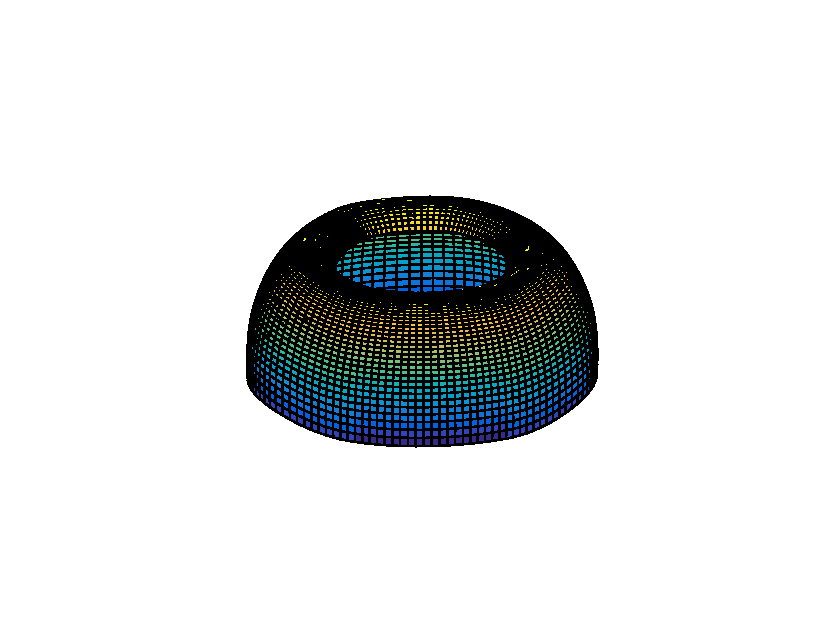
\includegraphics{Pictures/NURBS/fitting_pipeline/half_torus.eps}};
        \draw[thick,->] (N2) -- (N1);
        \draw[thick,->] (N3) -- (N2);
        \draw[thick,->] (N4) -- (N3);
       
\end{tikzpicture}
\end{frame}
%\begin{frame}{Before and after Peters}
%\vspace{-6mm}
%\begin{minipage}[t]{0.48\linewidth}
%\begin{block}{Before}
%\begin{figure}
%\includegraphics[width=0.8\linewidth]{uniform_hermite.eps}
%\end{figure}
%\end{block}
%\end{minipage}%
%\hfill%
%\begin{minipage}[t]{0.48\linewidth}
%\begin{block}{Legendre Chaos}
%\begin{itemize}
%\item[{\color{green}\smiley}] First order Legendre Chaos expansion represents the random variable \textit{exactly}.
%\vspace{5mm}
%
%\end{itemize}
%\begin{figure}
%\includegraphics[width=0.85\linewidth]{legendre_exact.eps}
%\end{figure}
%\end{block}
%\end{minipage}

%\end{frame}
\begin{frame}{Possible optimizations}
\begin{itemize}
\item Introduction of the \textit{fairness functional} in order to deal with more complex shapes
\item Implementation of the \textit{adaptive refinement} in order to control a maximum error tolerance
\item Implementation of the \textit{parameter correction} for the improved pipeline
\end{itemize}
\begin{figure}
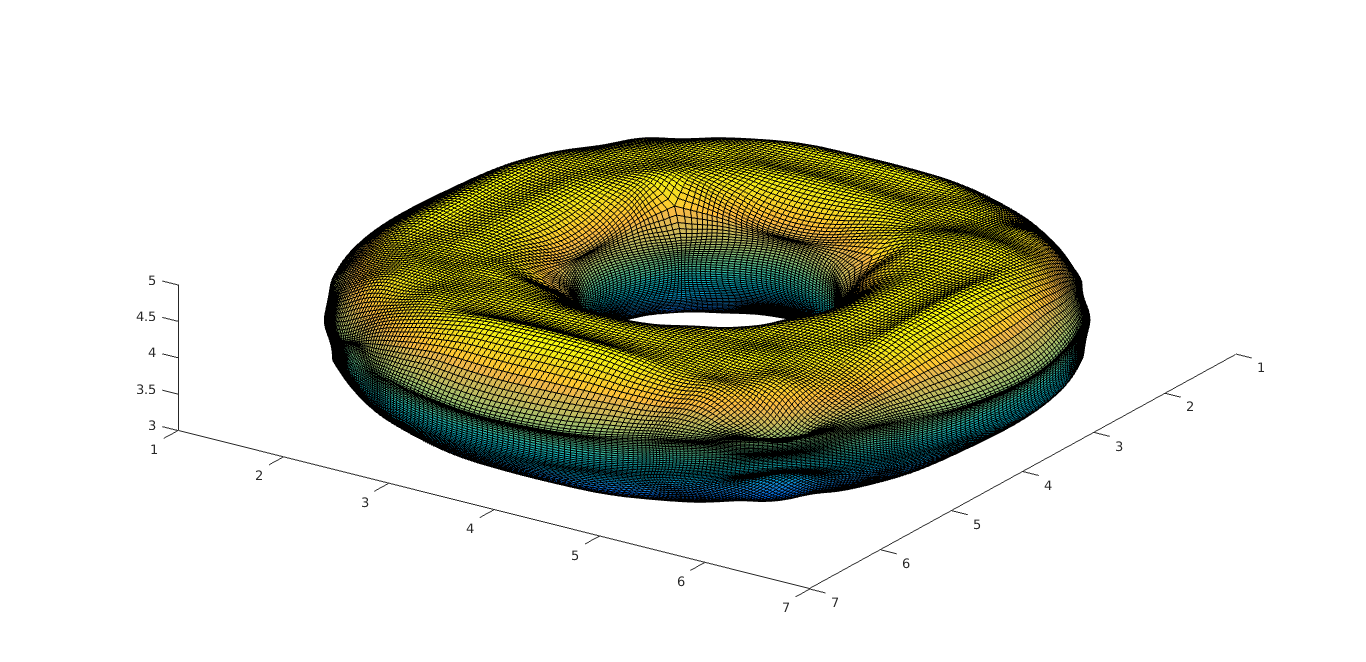
\includegraphics[width=\textwidth]{Pictures/NURBS/torus_from_DC.png}
\end{figure}
\end{frame}
\section{Summary \& Outlook}
%\begin{frame}{Third Milestone's achievements}
%%\begin{variableblock}{What's done?}{bg=cyan,fg=white}{bg=white,fg=black}
%%{
%
%
%
%\begin{itemize}
%	
%	\item[\textcolor{green}
%	{\Checkmark}] 100 \% open source
%	
%	\item[\textcolor{green}
%	{\Checkmark}] GUI for user interaction
%	
%	\item[\textcolor{green}
%	{\Checkmark}] Fairness functional to control Peters' scheme smoothness
%	
%		\item[\textcolor{green}
%	{\Checkmark}] Conversion back to CAD
%	
%	\item[\textcolor{green}
%	{\Checkmark}] Boolean operation support
%	
%	\item[\textcolor{green}
%	{\Checkmark}] Test Cases
%	
%	\item[\textcolor{green}{\Checkmark}] Fully integrated pipeline 
%
%
%\end{itemize}
%
%\end{frame}
%
%\begin{frame}{Outlook \& future work}
%\begin{itemize}
%\item Increase robustness of surface reconstruction \\
%{\footnotesize \textcolor{blue}{Big amount of work: include topology checks and guarantee correct ambiguity treatment}}
%\item Improve parameter estimation
%\begin{itemize}
%\item[--] complexity of algorithm \\ {\footnotesize \textcolor{blue}{current implementation has $\mathcal{O}\left(n^2\right)$ complexity}}
%\item[--] accuracy of result \\ {\footnotesize \textcolor{blue}{not always projection onto the correct patches}}
%\end{itemize}
%\item Determine approximation error for our algorithm
%\begin{itemize}
%\item[--] Topology checks\\ {\footnotesize \textcolor{blue}{see above}}
%\item[--] Accuracy estimates\\ {\footnotesize \textcolor{blue}{accuracy metrics? Important for estimation of reliability of results and basis for adaptivity}}
%\end{itemize}
%\item Develop a fully adaptive scheme \\ {\footnotesize \textcolor{blue}{Big amount of work: important for big patches and resolution of relatively small features, see testcase GE Bracket}}
%\item Exchange ToPy with a faster solution \\ {\footnotesize \textcolor{blue}{Important because ToPy is currently bottleneck, faster solution is available}}
%\end{itemize}
%\end{frame}
%\begin{frame}{Further remarks \& Discussion}
%\begin{itemize}
%\item \textcolor{blue}{isogeometric analysis as an completely different approach for the whole problems (anyhow there are many open questions)}
%\item \textcolor{blue}{isogeometric analysis for shape optimization after topology optimization?}
%\end{itemize}
%\end{frame}


\begin{frame}{Results}
\begin{figure}
%\vspace{-.7cm}	
%\hspace{-2cm}
		\includegraphics[width=1\linewidth]{Pictures/SecondHalf/TestCases.png}
		\end{figure}
GE Bracket design already optimized\textsuperscript{4} and only reconstructed.
\end{frame}

\begin{frame}{Summary}
\begin{variableblock}{What did we achieve?}{bg=cyan,fg=white}{bg=white,fg=black}
{
\begin{itemize}
	
	\item[\textcolor{green}
	{\Checkmark}] Fully working, fully open source prototype (with GUI!)
	
	\item[\textcolor{green}
	{\Checkmark}] Contract specifications fulfilled!
	
	\item[\textcolor{green}{\Checkmark}] No dropouts, no major fights, only moderate stress levels :-) 
	
	\item[\textcolor{green}{\Checkmark}] Fun and interesting project (and even a good grade)


\end{itemize}
}
\end{variableblock}
\end{frame}




%%%%%%%%%%%%%%%%%%%%%%%%%%%%%%%%%%%%%%%
%%%OLD SLIDES

%\begin{frame}{What is next?}
%\begin{variableblock}{What's done?}{bg=cyan,fg=white}{bg=white,fg=black}
%{
%\begin{itemize}

%\item<+-> Topology Optimization
%\begin{itemize}
%	\item[\textcolor{green}{\Checkmark}] Pipeline from CAD model to optimized voxel model
%	\item[\textcolor{green}{\Checkmark}] User input of boundary conditions
%	\item[\textcolor{black}{\VarClock}] Support for complex geometries
%	\item[\textcolor{red}{\XSolidBrush}] GUI for user interaction
%\end{itemize}

%\item<+-> Surface Extraction
%\begin{itemize}
%	\item[\textcolor{green}{\Checkmark}] Dual Contouring for simple geometries
%	\item[\textcolor{green}{\Checkmark}] Provide necessary data for Surface Fitting
%	\item[\textcolor{black}{\VarClock}] Interfaces
	%\item[\textcolor{red}{\XSolidBrush}] Adaptive and topology safe Dual Contouring
%\end{itemize}

%\item<+-> Surface Fitting
%\begin{itemize}
	%\item[\textcolor{green}{\Checkmark}] B--spline fitting using least squares
	%\item[\textcolor{green}{\Checkmark}] Smooth connection of patches using Peters' scheme
	%\item[\textcolor{red}{\XSolidBrush}] Conversion back to CAD
%\end{itemize}
%\end{itemize}
%}
%\end{variableblock}
%\end{frame}

















\section*{Thank You}
\begin{frame}{Thank you for your attention!}
	\begin{figure}
		\scalebox{0.12}{\includegraphics{Pictures/1CAD.pdf}}
		\scalebox{0.12}{\includegraphics{Pictures/2STL.pdf}}
		\scalebox{0.12}{\includegraphics{Pictures/3VOX.pdf}}
		\scalebox{0.12}{\includegraphics{Pictures/4TPD.pdf}}
		\scalebox{0.12}{\includegraphics{Pictures/5TOPOPT.pdf}}
		\scalebox{0.12}{\includegraphics{Pictures/6TOPYOUT.pdf}}
		\scalebox{0.12}{\includegraphics{Pictures/7MC.pdf}}
		\scalebox{0.12}{\includegraphics[scale=1.3]{Pictures/End.png}}
	\end{figure}
	\begin{figure}
	\includegraphics[scale=0.2]{Pictures/TheArc.png}
	\end{figure}
\end{frame}

\section*{Literature}
\begin{frame}{Literature}
\begin{itemize}
\item \textbf{William Hunter} Predominantly solid-void three-dimensional topology optimisation using open source software
\item \textbf{Gerrit Becker, Michael Sch\"afer, Antony Jameson.} "An advanced NURBS fitting procedure for post-processing of grid-based shape optimizations"
\item \textbf{Matthias Eck, Hugues Hoppe.} "Automatic Reconstruction of B-Spline Surfaces of Arbitrary Topological Type"
\end{itemize}
\end{frame}

\section*{Theory}
\begin{frame}{Projection and Parametrization on arbitrary quads}
\begin{overlayarea}{\textwidth}{.15 \textheight}
\begin{enumerate}
\item<1-> find least squares plane approximating quad
\item<2-> projection of datapoint onto plane
\item<3-> find corresponding parameters $\left[u,v\right] \in \left[0,1\right]^2$
\end{enumerate}
\end{overlayarea}
\begin{overlayarea}{\textwidth}{.85 \textheight}
\only<1>{
\begin{columns}
\column{.3\textwidth}
\begin{figure}
\includegraphics[width = \textwidth]{Pictures/BackupSlidesProjection/nonPlaneQuads.png}
\caption{DC sphere}
\end{figure}
\column{.3\textwidth}
\begin{figure}
\includegraphics[width = \textwidth]{Pictures/BackupSlidesProjection/withPlaneQuads.png}
\caption{with plane quads}
\end{figure}
\end{columns}
}
\begin{columns}
\column{.35\textwidth}

\begin{overlayarea}{\textwidth}{\textheight}
\begin{figure}
\only<2-3>{
\tdplotsetmaincoords{60}{110}
\begin{tikzpicture}[scale = 1.5,tdplot_main_coords]
\coordinate (O) at (-1,-1,0);
\coordinate[dot] (A) at (0,0,0);
\coordinate[dot] (B) at (1,0,0);
\coordinate[dot] (C) at (1.2,1.5,0);
\coordinate[dot] (D) at (0,1,0);
\coordinate (P1) at (.5,.4,1);
\coordinate (P2) at (1,1,1);
\coordinate (Q1) at (.5,.4,0);
\coordinate (Q2) at (1,1,0);

\draw[thick,->] (O) -- ($(O)+(.5,0,0)$) node[anchor=north east]{$x$};
\draw[thick,->] (O) -- ($(O)+(0,.5,0)$) node[anchor=north west]{$y$};
\draw[thick,->] (O) -- ($(O)+(0,0,.5)$) node[anchor=south]{$z$};

\draw[thick] (A) -- (B) -- (C) -- (D) -- (A);

\only<2-3>{
\draw (P1) node[thick,cross,red,label = {$P_1$}] {};
\draw[red,dashed] (P1) -- (Q1);
\draw (Q1) node[thick,cross,red] {};
}
\only<3>{
\draw (P2) node[thick,cross,red,label = {$P_2$}] {};
\draw[red,dashed] (P2) -- (Q2);
\draw (Q2) node[thick,cross,red] {};
\draw[black,dashed] (B) -- (D);
}
\draw (A) node[label = left:{$A$}]{};
\draw (B) node[label = left:{$B$}]{};
\draw (C) node[label = right:{$C$}]{};
\draw (D) node[label = right:{$D$}]{};
\end{tikzpicture}
}
\end{figure}
\end{overlayarea}

\column{.5\textwidth}
\begin{overlayarea}{\textwidth}{\textheight}
\only<2>{
\begin{block}{Coordinate transformation}
system with basis
\begin{equation*}
B_{BAD} = \left(
\begin{array}{ccc}
\vec{n} & \vec{AB} & \vec{AD}
\end{array}
\right)
\end{equation*}
yields
\begin{equation*}
\left(B_{BAD}\right)^{-1} P_1
=
\left(
\begin{array}{ccc}
d&u&v
\end{array}
\right)^T
\end{equation*}
\end{block}
}
\only<3>{
\begin{block}{Problem:}
\begin{itemize}
\item[\textcolor{green}{\Checkmark}] for $P_1$: $\left(u,v\right) = \left(0.5,0.4\right)$
\item[\textcolor{red}{\XSolidBrush}] for $P_2$: $\left(u,v\right) = \left(1,1\right)$
\end{itemize}
\end{block}

\begin{block}{Solution:}
\begin{enumerate}
\item if we get $u+v > 1$
\item use $B_{BCD}$ instead of $B_{BAD}$
\item set $u=1-u$, $v=1-v$
\end{enumerate}
\end{block}

}
\end{overlayarea}
\end{columns}
\end{overlayarea}
\end{frame}

\end{document}
